\section{Grundlagen}

Bevor es ans Fechten geht, gilt es einen grundlegenden Rahmen abzustecken, auf den sich alle Fechtenden gleichermaßen beziehen können. Dies betrifft zum einen das Vokabular, sodass bei der Kommunikation untereinander keine Missverständisse entstehen. Es betrifft aber auch die Regeln zum Umgang miteinander und den Umgang mit den Fechtstücken, um zu gewährleisten, dass alle mit den gleichen Erwartungen trainieren können. Daher empfiehlt es sich, die nachfolgenden Kapitel aufmerksam zu lesen, auch wenn Einiges darin sicher bereits bekannt ist.

\subsection{Trainingsmaxime}

\subsubsection*{I. Keine Interpretation ist perfekt!}

Da sich HEMA – also Historical European Martial Arts (engl. für ”historisch-europäische Kampfkünste”) nicht in einer lebendigen Tradition bewegt, sind alle Interpretationen zwangsläufig Auslegungen einer Schrift- und/oder Bildquelle, die Ungenauigkeiten oder Fehler enthalten können. Es ist also nicht überprüfbar, wie gut eine gefundene Interpretation der Intention des Autors entspricht.
\\
\\
Als Anfänger:in ist es deshalb sinnvoll, zunächst den Erklärungen der Trainer:innen zu
folgen. Mit zunehmender Erfahrung (bei regulärem Trainingsbesuch nach ca. 1 Jahr) können
eigene Interpretationsversuche unternommen werden.
\\
\\
Wichtig ist: Unsere Interpretationen entwickeln sich ständig weiter. Wir probieren Dinge aus,
hinterfragen sie und passen sie an. Dieser Prozess hört nie auf, das Ergebnis ist daher nie
perfekt.

\subsubsection*{II. Passt die Stücke an euch an!}

Jeder Mensch bringt andere Voraussetzungen mit. Größe, Reichweite, Kraft, Beweglichkeit und Vorerfahrungen beeinflussen, wie eine Technik funktioniert.
\\
\\
Deshalb sollten die gezeigten Techniken der Trainer:innen nicht einfach kopiert werden, sondern die Fechtenden sollen lernen, diese für sich nutzbar zu machen. Die Grundprinzipien bleiben gleich, aber die genaue Ausführung kann von Person zu Person
unterschiedlich aussehen.
\\
\\
Mit genügend Erfahrung können auch eigene Interpretationen der Techniken entstehen.

\subsubsection*{III. Fechtstücke sind nicht universal!}

Die nachfolgend beschriebenen Fechtstücke zeigen exemplarisch bestimmte Prinzipien oder typische Situationen. Sie sind nicht als universelle Lösungen gedacht und sollten immer als Anwendung eines zugrundeliegenden Fechtprinzips aufgefasst werden.
\\
\\
Fechtende sollten versuchen nicht nur die Technik auswendig zu lernen, sondern verstehen, warum sie funktioniert. Das zugrunde liegende Prinzip ist oft wichtiger als die genaue Bewegung.

\subsubsection*{IV. Miss dich nicht an anderen!}

Historisches Fechten kann zwar wettkampforientiert sein, aber ein Vergleich mit anderen ist oft kontraproduktiv.
\\
\\
Achte darauf, wie du dich entwickelst, welche Fortschritte du machst und woran du noch arbeiten möchtest. Sich ständig mit anderen zu vergleichen, hilft für einen kontinuierlichen Lernprozess meistens nicht weiter.
\\
\\
Dies sollte sich auch im Umgang miteinander zeigen. Kommentare, die andere bewerten oder vergleichen, kommen oft anders an als beabsichtigt und können beispielsweise als abwertend aufgefasst werden. Stattdessen wollen wir offen, respektvoll und unterstützend miteinander umgehen: Das Training ist kein Wettkampf!
\\
\\
Das Training gibt die Möglichkeit, Fehler zuzugeben, Fragen zu stellen und gemeinsam besser zu werden.

\subsubsection*{V.  Du trägst dazu bei, dass Andere vorankommen!}

Fechten lernt man nicht allein. Gute und kooperative Trainingspartner:innen sind eine der wichtigsten Voraussetzungen für Fortschritt.
\\
\\
Jede Übung sollte fordern, aber nicht überfordern. Deshalb tragen alle Verantwortung dafür, eine gute Lernatmosphäre zu schaffen – für sich selbst und für andere.
\\
\\
Im Training sind alle gleichzeitig Lernende und Lehrende. Erfahrenere Fechter:innen sollten ihr Verhalten an das Niveau ihrer Partner:innen anpassen und ihnen ermöglichen, sinnvoll zu üben.
\\
\\
Als grobe Faustregel gilt: Eine Übung sollte oft gelingen, aber nicht immer. Wenn sie ungefähr in 70\% der Versuche erfolgreich ist, liegt die Schwierigkeit meist genau richtig, um den bestmöglichen Lernfortschritt zu bieten.

\newpage

\subsection{Sicherheit}

Sicherheit stellt aus offensichtlichen Gründen die höchste Priorität beim Training im historischen Fechten dar. Darüber hinaus ist Sicherheit aber auch Voraussetzung für effektives Training, denn verletzte Fechter:innen können nicht effektiv am Training teilnehmen. Trainieren mit übersteigerter Härte, mangelnder Kontrolle oder mangelnder Schutzausrüstung für schnellere Fortschritte ist also widersprüchlich.
\\
\\
Nichtsdestotrotz kann es zu Unfällen kommen. In diesem Fall sollten selbst leichte Verletzungen unmittelbar einem:einer Trainer:in und im Anschluss an das Training einem Mitglied des Vorstandes gemeldet werden. Dieser Nachweis ist insbesondere aus versicherungsrechtlichen Gründen erforderlich. Jede:r Fechter:in kann sich zudem jederzeit nach eigenem Empfinden selbst aus dem Training entfernen, wenn er:sie dies für sinnvoll hält. Trainieren trotz einer Verletzung stellt eine Gefahr für den:die Fechter:in selbst, sowie dessen Trainingspartner:in dar und ist keine effektive Weise, zu trainieren.
\\
\\
Im folgenden Abschnitt werden einige Regeln genannt, die ein sicheres Training gewährleisten sollen. Diese Regeln sollten als Referenz für sicheres Verhalten verstanden werden und ersetzen weder die Einschätzung eines:einer Trainer:in, noch sind sie eine völlige Schadenfreiheitsgarantie. Falls bezüglich der Sicherheit einer Übung oder ähnlichem Zweifel besteht, fragt unbedingt einen:eine Trainer:in!
\\
\\
\textbf{Regeln für sicheres Training}

\begin{enumerate} [I.]
\item Passt eure Geschwindigkeit eurer Fähigkeit, die Klinge zu kontrollieren an! Ihr solltet die Klinge auch im Hau noch stoppen können!
\item Passt eure Schutzausrüstung den verwendeten Schwertsimulatoren und der Übung an! Polsterschwerter und Plastikwaster können auch nur mit Maske verwendet werden, während Stahlschwerter für unkooperatives Training eine volle Schutzausrüstung benötigen.
\item Passt die Komplexität einer Übung dem:der unerfahreneren Fechter:in an! Ein:e überforderte:r Fechter:in macht häufiger Fehler und trägt nicht zu sicherem Verhalten bei. Kommuniziert klar, wenn ihr die Intensität der Übung anpassen möchtet.
\item Wendet nie mehr, als die notwendige Härte für eine Übung an! Eine hohe Härte ist für sehr wenige Übungen notwendig.
\item Nutzt die Schutzausrüstung, die ihr tragt möglichst optimal. Schlagt nie bewusst in Lücken der Schutzausrüstung!
\item Vermeidet Häue und Stiche in sensible Gegenden, wie den Schritt oder die Rippen, besonders wenn diese ungeschützt sind!
\item Seid immer transparent über Verletzungen, eure Fähigkeit, sicher zu trainieren oder andere Zweifel bezüglich der Sicherheit einer Übung!
\end{enumerate}

\newpage

\subsection{Ausrüstung}

Für den Einstieg ins Training genügt einfache Sportkleidung und ggf. Hallenschuhe. Je nach persönlicher Präferenz können auch dünne Fahrrad- oder Lederhandschuhe getragen werden.

\paragraph{Achtung!}
Konsultiert vor der Anschaffung von Ausrüstung unbedingt einen:eine Trainer:in, um teure Fehlkäufe zu vermeiden. Auch andere Vereinsmitglieder haben häufig wertvolle Erfahrung mit Herstellern und Ausrüstungsgegenständen.

\subsubsection*{\hspace{3.75cm}Empfohlene Ausrüstung Anfänger:}

\begin{longtable}{p{6.25cm}p{6.25cm}}
Leihausrüstung:
\begin{itemize}
 \item Fechtmaske
 \item Plastikschwert
 \item ggf. Stahlschwert/-feder
 \item ggf. Schutzhandschuhe
\end{itemize}

&

Erweiterte Ausrüstung zum Selbstkauf:
\begin{itemize}
 \item Fechtmaske (1600N, FIE Niveau 2)
 \item Stahlschwert/-feder (Flex von 12-13kg)
 \item HEMA-Schutzhandschuhe aus überlappenden, harten Elementen (Polsterhandschuhe sind nicht ausreichend)
 \item Halsschutz
\end{itemize}
\end{longtable}

\subsubsection*{\hspace{3.5cm}Empfohlene Ausrüstung Fortgeschrittene:}

\begin{longtable}{p{6.25cm}p{6.25cm}}
Mindestausrüstung zur Teilnahme:
\begin{itemize}
 \item Fechtmaske (1600N, Niveau 2)
 \item Stahlschwert/-feder
 \item HEMA-Schutzhandschuhe aus überlappenden, harten Elementen (Polsterhandschuhe sind nicht ausreichend)
 \item Fechtjacke (800N Stichschutz)
 \item Halsschutz
\end{itemize}

&

Empfohlene Ausrüstung für Sparring:
\begin{itemize}
 \item alle zuvor aufgeführten Gegenstände
 \item Fechthose ($\geq$ 350N Stichschutz)
 \item Tiefschutz
 \item Plastron
 \item Hinterkopfschutz für Fechtmaske
 \item Ellbogenschutz
 \item Ober- \& Unterarmschutz
 \item Knieschutz
 \item Schienbeinschutz (bestenfalls mit Schutz für Fußgelenke)
\end{itemize}
\end{longtable}

\subsubsection*{Worauf sollte ich achten?}

Um die Verletzungsgefahr gering zu halten, darf eure Ausrüstung nicht aus Metall sein oder keine größeren freiliegenden Metallteile haben (außer dem Gitter der Fechtmaske). Achtet grundsätzlich darauf, dass eure Ausrüstung zusammenpasst. Zum Beispiel kann der Unterarmschutz mit dem Handgelenkschutz der Handschuhe kollidieren. Zu viele (mehr als zwei) Lagen übereinander schränken die Beweglichkeit meist stark ein und können zu Wärmestau führen. Generell ist immer ein Kompromiss aus Schutz, Beweglichkeit und Wärmemanagement zu finden. Das Ziel kann je nach körperlichen Voraussetzungen und natürlich Trainings- bzw. Wettkampfmodus variieren. Den Schutzlevel variabel zu gestalten ist vorteilhaft, da verschiedene Trainingsmodi unterschiedliche Ausrüstung erfordern. Allerdings sollte jeder in der Lage sein, seine Ausrüstung ohne größere Hilfe in überschaubarer Zeit (ca. 5min) selbst anzulegen.
\\
\\
Es folgen einige Hinweise für die Ausrüstungswahl. Produktempfehlungen gibt es separat, da sich diese sich mit neuen Erfahrungen und neu verfügbaren Ausrüstungen schnell ändern können.

\newpage

\subsubsection*{Schuhe}

\begin{itemize}
    \item abriebfreie Hallenschuhe, möglichst mit heller Sohle und abgerundeten Hacken (aus modernem Fechtsport, Ringen oder anderen Hallensportarten)
\end{itemize}

\subsubsection*{Fechtmaske}

\begin{itemize}
    \item FIE 1600N Zertifizierung, Niveau 2
    \item Passform: Die Maske sollte unter dem Kinn eng anliegen, aber nicht schmerzhaft sein; Masken sind begrenzt verformbar, um sie individuell anzupassen.
    \item Masken sollten ein Stirnband als Schutz gegen das Hineinrutschen ins Schutzgitter besitzen.
    \item Das Unterziehen einer Polsterhaube aus dem Rugby ist möglich (mehr Schutz bei harten Treffern, eventuell größere Maske nötig).
\end{itemize}

\subsubsection*{Handschuhe}

\begin{itemize}
    \item Passform: Die Faust sollte in geschlossener Position entspannt sein und beide gängigen Griffweisen sollten bequem ausführbar sein. (Manche Huten und Positionen unterliegen selbstverständlich Einschränkungen)
    \item Die Handschuhe sollten aus überlappenden harten Elementen bestehen.
    \item Fingerhandschuhe sind immer ein Kompromiss in Dingen Sicherheit. In einzelnen Fällen \textbf{können} sie die Beweglichkeit der Finger verbessern. Tendentiell sind Fausthandschuhe allerdings immer sicherer. Zur Zeit sind keine auf dem Markt befindlichen Fingerhandschuhe für hartes Sparring empfehlenswert.
\end{itemize}

\subsubsection*{Halsschutz/Stechlatz:}

\begin{itemize}
    \item Passform: Der Halsschutz sollte unter der Fechtjacke eng am Hals anliegen, ohne die Atmung zu behindern oder den Träger zu würgen.
    \item Jeder Halsschutz muss harte Elemente am Kehlkopf besitzen.
    \item Den Halsschutz gibt es in Varianten ohne zusätzlichen Schutz, mit Stechlatz und mit Stechlatz und mit zusätzlichem Schlüsselbein-/Schulterschutz.
\end{itemize}

\newpage

\subsubsection*{Stahlschwert/Stahlfeder - Langes Schwert}

\paragraph{Achtung!}
Hier kann man wirklich viel falsch machen: Fragt unbedingt eure Trainer:innen! Wenn möglich wird zudem empfohlen, mögliche Modelle im Voraus persönlich zu testen. Fragt hierzu gerne im Verein rum, dort sind viele verschiedene Federn vertreten.

\paragraph{Dimensionen:}
\begin{itemize}
    \item Die Gesamtlänge sollte der Körpergröße angepasst sein (vom Boden bis etwa zwischen Brustbein und Brustwarze). Zu lange Schwerter können saubere Techniken behindern!
    \item Die Grifflänge sollte (inklusive Knauf) etwa zwischen 27 und 32 cm betragen. Längen über 34cm behindern vor allem Techniken des Ringens (am Schwert). Mit Handschuhen sollten dennoch beide Hände zwischen Kreuz und Knauf passen.
    \item Das Gewicht sollte sich bei ca. 1,4kg-1,5kg orientieren und nach persönlicher Präferenz drüber oder drunter liegen. Wichtig: Auch zu leichte Federn können das saubere Erlernen von Techniken behindern!
\end{itemize}

\paragraph{Sicherheit:}
\begin{itemize}
    \item Der Ort sollte umgeschlagen oder zumindest verdickt sein, um im Stich nicht gefährlich zu sein. Sicherheitsstandards tendieren zunehmend zum umgeschlagenen Ort.
    \item Die Schlagkante sollte mind. 2-3 mm nahe des Orts und zum Kreuz hin min 5 mm Dicke aufweisen und abgerundet sein.
    \item Das Schwert muss sich bei einer Belastung von ca. 12kg-13kg sichtlich durchbiegen, um Sicherheit im Stich zu gewährleisten.
    \item Knauf, Kreuz, Schilt und Klinge dürfen keine scharfen Kanten oder Ecken haben.
\end{itemize}

\paragraph{Konstruktion:}
\begin{itemize}
    \item Der Knauf sollte mit der Klinge vernietet sein. Geschraubte Verbindungen lösen sich leicht und können zum Bruch der Angel führen.
    \item Von Parierringen (Seitenringen) am Kreuz wird stark abgeraten. Sie behindern bestimmte Techniken und bieten ein Sicherheitsrisiko beim Ringen (fallen auf am Boden liegendes Schwert). Sie sind zudem in Wettkämpfen häufig nicht erlaubt.
\end{itemize}

\newpage

\subsubsection*{Fechtjacke}

\begin{itemize}
    \item 800N Stichfestigkeit (Stoff)
    \item Passform: Die Fechtjacke sollte gute Beweglichkeit bieten. Beide Arme sollten leicht über den Kopf zu heben sein und dabei die Unterkante der Jacke nicht signifikant heben. Der Klingenfang am Hals sollte nicht würgen.
    \item Gambesons erfüllen \textbf{nicht} die Anforderungen einer Fechtjacke (oft ohne Stichfang, keine 800N Stichfestigkeit und häufig Öffnung vorn).
    \item Der Verschluss sollte vorn bzw. seitlich ausreichend überlappen.
    \item Ein Stichfang am Hals (Stofftasche in die die Schwertspitze rutsch, wenn ein Stich unter Maske rutscht) wird stark empfohlen.
    \item Achtung: Stichfestigkeit sagt nichts über Polsterwirkung gegen stumpfe Gewalteinwirkung aus! Zusätzliche Protektoren und ein Plastron sind hierfür notwendig.
    \item Jacken mit guter Polsterung sind häufig schwer und schränken Beweglichkeit und Wärmeableitung ein. Schutz, Beweglichkeit und Wärmeabführung müssen abgewogen werden!
    \item Es gibt Jacken mit eingebauten Schutzelementen. Vorteile: kein mühsames Anlegen der Extrapanzerung, kein Abschnüren von Gliedmaßen durch Klettverschlüsse; Nachteile: möglicherweise unflexibel im Schutzgrad (nicht bei allen Übungen wird volle Rüstung gewünscht), bei Beschädigung schwer austauschbar
    \item Jacken sollten waschbar sein!
\end{itemize}

\subsubsection*{Hinterkopfschutz/Maskenüberzug}

\begin{itemize}
    \item Passform: Er sollte eng und sicher auf Maske sitzen, Sicht und Beweglichkeit aber nicht zu stark einschränken.
    \item Maskenüberzüge schützen Kopf \textbf{und} Maske.
\end{itemize}

\subsubsection*{Ellenbogen-/Unteram-/Knie-/Schienbeinschutz}

\begin{itemize}
    \item Alle Protektoren sollten harte Elemente enthalten, die bestenfalls überlappen.
    \item Es gibt Ellenbogenschutz für über und andere für unter die Fechtjacke.
\end{itemize}

\hfill
\\
Wichtig für Turnierfechtende:
\\
DDHF Regelwerk: https://www.ddhf.de/turniere/regelwerke/

\subsection{Allgemeine Lehre}

In europäischer Geschichtsschreibung tauchen immer wieder spezielle Formen des ritualisierten Zweikampfes auf. Deren Zwecke sind vielfältig und reichen von sportlichem Wettbewerb und persönlicher Freizeitgestaltung über gerichtliche Ergebnisfindung bis zu gewaltsamer, nicht-institutionalisierter Konfliktaustragung. Alle zu dieser Form des Zweikampfes gehörenden Disziplinen für den Kulturraum Europa werden unter dem Sammelbegriff HEMA (Historical European Martial Arts) zusammengefasst. Wir als historische Fechter:innen befassen uns mit dem speziellen Teilgebiet dieser, welches sich vor allem auf die Verwendung von Klingenwaffen, stumpfen Waffen (z.B. der halben Stange) sowie den waffenlosen Kampf (z.B. Ringen) fokussiert.

\subsubsection{Quellen}

Die heutige HEMA-Gemeinde befindet sich im engeren Sinne nicht in einer lebendigen Tradition. Es gibt also keine ununterbrochen praktizierte Überlieferung der mittelalterlichen/frühneuzeitlichen europäischen Kampfkünste. Der Grund hierfür liegt in der kontinuierten Weiterentwicklung der Waffen. Veränderungen in Waffe und Führungsweise bedingten sich gegenseitig und transformierten so beide nachhaltig. Dies kulminierte in der Redundanz des Schwertes sowohl im militärischen wie auch dem zivilen Kontext Anfang des 20.Jahrhunderts. Weiter überlebte die Kampfkunst nur in Form des modernen Sportfechtens, welches zwar technisch gesehen eine lebendige Tradition nachweisen kann, die sich bis ins Mittelalter zurück verfolgen lässt, mit der Kampfkunst dieser Zeit allerdings sehr wenig gemeinsam hat. Deshalb ist es für das Nachvollziehen der Lehre notwendig, auf die Quellen (z.B.: Schrift-, Bildquellen, erhaltene zeitgenössische Waffen und Ausrüstug, Grabsteine, Knochenfunde) aus Mittelalter und Früher Neuzeit zurückzugreifen.
\\
\\
Als ältestes in Europa erhaltenes Kampfbuch des Mittelalters gilt das sogenannte ''Tower Fechtbuch'', benannt nach seinem Aufbewahrungsort im Tower of London (oder auch I.33 nach seiner Inventarnummer). Es wurde wahrscheinlich von bayrischen Mönchen in den 1320ern geschrieben und beschreibt vornehmlich den Umgang mit Einhandschwert und Buckler (einem kleinen Faustschild). Für das Lange Schwert im europäischen Raum beginnt die schriftliche Überlieferung mit zwei grundlegenden Traditionssträngen zu Beginn des 15. Jahrhunderts: ''Fior di Battaglia'' (italienisch für ''Blume der Schlacht'', Inv. Nr.: Ms. M.383) von Fiore Furlano de'i Liberi und Johannes Liechtenauers Merkverse. Beide gelten heute als Begründer der jeweiligen Fechttraditionen (auch ''Schulen'') ihrer Sprachräume (italienisch und deutsch), welche bis heute als die wichtigsten Fechttraditionen für das Lange Schwert angesehen werden.
\\
\\
Für uns als Fechter:innen am Langen Schwert nach der deutschen Schule ist vor allem Liechtenauer relevant. Von ihm selbst sind keine Schriftzeugnisse bekannt, viele deutschsprachige Kampfbücher überliefern jedoch fechterische Merkverse, die auf ihn zurückgehen sollen und als verbindendes Element der Liechtenauerschen Tradition wirken. Da diese wohl ursprünglich auf Notizzetteln (sog. „zedel“) überliefert wurden, wurde dieser Begriff mit der Zeit zu einem Synonym für Liechtenauers Verslehre. Liechtenauers „zedel“ sollte eingeweihten Fechtern und Fechtlehrern als Gedankenstütze und zur Strukturierung des Unterrichts dienen und ist daher in einer für Außenstehende nur sehr schwer verständlichen Sprache voller Fachbegriffen und Verknappungen verfasst, welche ohne erläuternden Kommentar nicht zugänglich ist. Allerdings gibt es eine große Zahl an Werken späterer Fechtmeister, die sich explizit auf Liechtenauer beziehen, meist sogar eine Form der „zedel“ enthalten und diese mit Anmerkungen, sog. „Glossen“, kommentieren. Dies ist auch der Grund, aus dem er als Begründer einer deutschen Schule betrachtet werden kann. In diversen Werken wird Liechtenauer als Legende beschrieben: Er habe sein Wissen von Reisen durch alle Höfe Europas erlangt. Deshalb ist zum einen davon auszugehen, dass  bereits vor 1400 eine nicht niedergeschriebene, oder zumindest nicht schriftlich erhaltene, Fechtkultur bestand. Zum anderen aber auch, dass es sehr wahrscheinlich einen Austausch zwischen den Lehrenden gab. Selbiges wird auch dadurch gestützt, dass sich in beiden Schulen viele Stücke stark ähneln.
\\
\\
Im Anhang ist eine ausführliche Auflistung von Quellen in der Tradition Johann Liechtenauers zu finden. Für den hier präsentierten Kanon wird sich zumeist aus den Stücken eines anonymen Glossators (mitunter als „Pseudo-Peter von Danzig bezeichnet“) zu Liechtenauers Merkversen (Rom, Biblioteca dell'Accademia Nazionale dei Lincei e Corsiniana, Cod. 1449 (Standortnummer 44 A 8), datiert: 1452) für das Lange Schwert und Fabian von Auerswalds ''Ringer Kunst: funf und achtzig Stücke'' (Göttingen, Staats- und Universitätsbibliothek, 2° Cod. Ms. philos. 62, datiert: 1537) für das Ringen bedient. Des Weiteren ist für das Lange Schwert und das Ringen auch das in der SLUB in Dresden aufbewahrte Mscr.Dresd.C.487 zu nennen, welches größtenteils Sigmund Ringeck zugeschrieben wird. Weitere in der SLUB aufbewahrte Manuskripte befassen sich vorrangig mit dem Stoßfechten.

\subsubsection{Das Schwert}

\FloatBarrier

\begin{figure}
    \centering
    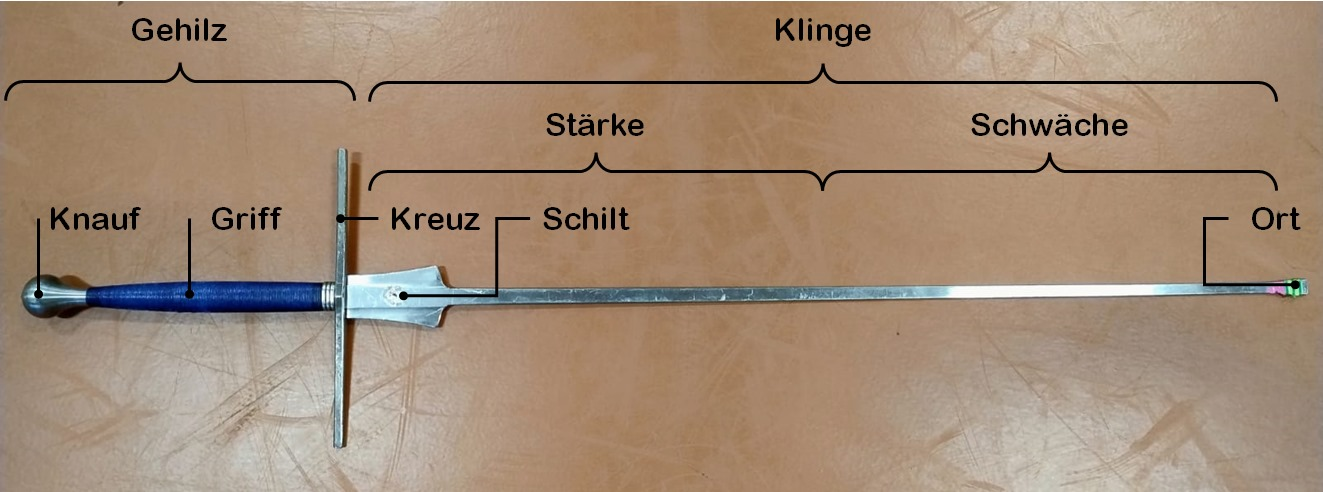
\includegraphics[scale=.35]{Nomenklatur.jpg}
    \caption{Die Nomenklatur des Schwertes}
    \label{fig:Schwert1}
\end{figure}

In \ref{fig:Schwert1} ist die Nomenklatur für das Schwert abgebildet. Die Klinge des Schwertes wird sowohl in Stärke und Schwäche, als auch in lange und kurze Schneide unterteilt. Beide Unterteilungen sind für die Bindungsarbeit wichtig und werden deshalb in den Kapiteln \ref{Bindung0} und \ref{Bindung1} ausführlich behandelt.

\FloatBarrier

\begin{figure}[ht!]
\minipage{0.38\textwidth}
  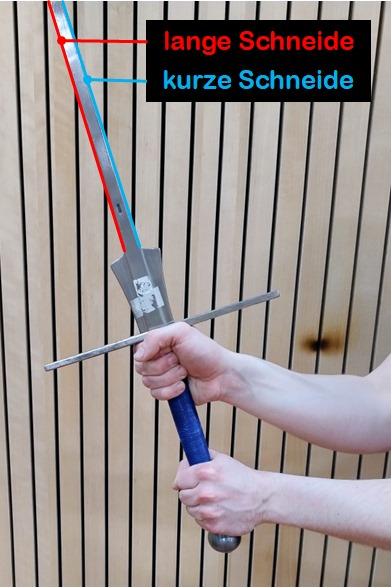
\includegraphics[width=\linewidth]{Hammergriff.jpg}
  \caption{Hammergriff}\label{fig:Hammergriff}
\endminipage\hfill
\minipage{0.38\textwidth}
  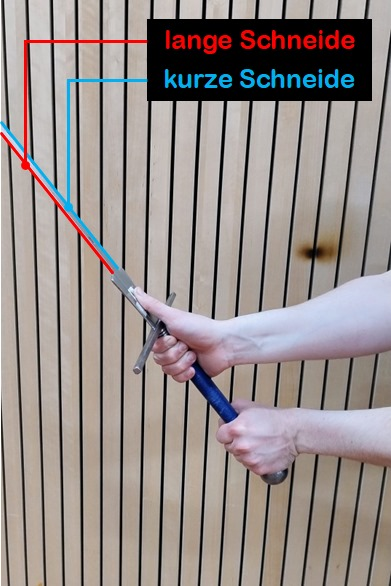
\includegraphics[width=\linewidth]{Daumengriff.jpg}
  \caption{Daumengriff}\label{fig:Daumengriff}
\endminipage\hfill
\end{figure}

Die Griffweise des Schwertes ist variabel. Die dominante Hand greift das Schwert am Griff, nahe des Kreuzes. Für diese Hand gibt es zwei grundlegende Griffweisen. Die erste kann als Hammergriff bezeichnet werden, bei dem bei dem die dominante Hand den Griff so greift, dass die Daumengabel in Linie mit dem Kreuz liegt. Die andere Griffweise heißt Daumengriff. Beim Daumengriff greift die dominante Hand den Griff so, dass der Daumen flach auf dem Kreuz oder Schilt liegt. Die zweite Hand umfasst in beiden Griffweisen den Griff im hinteren Drittel oder am Knauf und kann ihre Position verändern, sodass sich die Griffweise stets ergonomisch (niemals schmerzhaft!) anfühlt.
\\
\\
Die Unterteilung in Stärke und Schwäche richtet sich nach der Hebelwirkung, welche man mit der Klinge ausüben kann. Je länger der angewandte Lastarm wird, desto weniger Kraft kann man übertragen. Deshalb wird die Hälfte des Schwertes, welche weiter vom Hebelpunkt (dem Kreuz) entfernt ist, als Schwäche bezeichnet. Die näher am Kreuz gelegene Hälfte wird analog als Stärke bezeichnet. Das resultierende Kräfteverhältnis ist entscheidend für viele Fechtstücke.
\\
\\
Die Unterteilung in kurze und lange (manchmal ''wahre'' und ''falsche'') Schneide ist ebenfalls in der Bindungsarbeit wichtig und entspringt möglicherweise der Bezeichnung von Klingen (Säbel, Falchion), die tatsächlich zwei unterschiedlich lange Schneiden besitzen. Entsprechend der Griffweise dieser Waffen wird die Klinge, welche im Hammergriff in Richtung der Fingerknöchel zeigt stets als lange Schneide, und die Klinge welche in Richtung der Daumengabel zeigt als kurze Schneide bezeichnet. Im Daumengriff liegt die lange Schneide an den vordersten Fingerknöcheln, die kurze am Handrücken.

\subsubsection{Huten}

In der Tradition Liechtenauers werden vier Grundhaltungen unter dem Namen ''Hut'' (seltener Leger oder Lager) beschrieben. In diesen Huten schützt das Schwert jeweils einen klar definierten Bereich des Körpers, was dem Gegenüber nur begrenzte Möglichkeit gibt, durch eine direkte Aktion einen Treffer zu setzten. Gleichzeitig begünstigt die eigene Schwerthaltung manche Fechtstücke und erschwert andere. Das Wissen über die Möglichkeiten sowie Vor- und Nachteile der einzelnen Huten macht ein Gefecht berechenbarer und erleichtert den Eigenschutz. Es wird daher empfohlen, sich während des Gefechts dynamisch innerhalb dieser Huten zu bewegen und  diese als Anfangs- und Endpunkt der eignen Aktionen nutzen.
\\
\\
Liechtenauer und seine Anhänger unterscheiden also die vier grundlegenden Huten:
\enlargethispage{2\baselineskip}
\begin{itemize}
\item Vom Tag
\item Ochs
\item Pflug
\item Alber (seltener Alba oder Olber)
\end{itemize}

\hspace{1cm}
\\
Neben den Grundhuten werden später weitere Nebenhuten eingeführt (siehe Kap. \ref{Unten} und Kap. \ref{Wunder}), welche teils Übergangspositionen in Fechtstücken oder Ausgangsgangspunkt für spezielle Fechtstücke (meist in Tradition Liechtenauers aus der frühen Neuzeit) darstellen.
Auch viele der Grundhuten können anhand der Schwertstellung weiter differenziert werden (Links / Rechts / Neutral). Wird in Texten keine Spezifizierung genannt, ist im Zweifel meist die neutrale oder rechte Variante gemeint.
\\
\\
Die Interpretation der Huten erfolgt größteils aus Bildquellen. Gemäß Maxime II sollte auch jeder für sich eine möglichst ergonomische und kraftsparende Auslegung finden. Nachfolgend ist jedoch eine kurze Bilderfolge der derzeitig prominentesten Interpretationen abgebildet.

\newpage

Als allgemeine Körperhaltung haben sich für alle Huten einige Gemeinsamkeiten etabliert.

\begin{itemize}
    \item Die Füße stehen etwas weiter als hüftweit, und zueinander etwa einen Gehschritt versetzt, um Gleichgewichtsverschiebungen schnell entgegentreten zu können.
    \item Beide Fußsohlen bleiben vollständig auf dem Boden.
 \item Wird das Schwert auf einer Seite gehalten, sollte stets der gegenüberliegende Fuß vorne stehen, um die Haubewegung besser unterstützen zu können.
 \item Der vordere Fuß zeigt zum Gegenüber (oder leicht nach außen), die hintere Fußspitze ist nach außen gedreht.
 \item Die Hüfte ist in den meisten Huten zum:zur Gegner:in ausgerichtet, sodass keine Hüftseite übermäßig zum Gegenüber zeigt. Außerdem ist sie leicht abgesenkt, sodass sich die Beine in eine minimale Hockbewegung begeben und dadurch leicht angespannt sind.
 \item Der Oberkörper ist gerade und leicht nach vorn gebeugt.
 \item Die Brustlinie richtet sich ebenfalls zum Gegnüber aus, sodass keine Schulter übermäßig zum:zur Gegner:in zeigt.
 \item Die Schultern sind leicht angespannt, sodass der Rücken keinen Buckel, aber auch kein Hohlkreuz bildet.
 \item Die Arme (speziell die Ellenbogen) bleiben nah am Körper, um kein Ziel zu bieten.
\end{itemize}

\newpage

\paragraph{Vom Tag}

\begin{figure}[ht!]
\minipage{0.32\textwidth}
  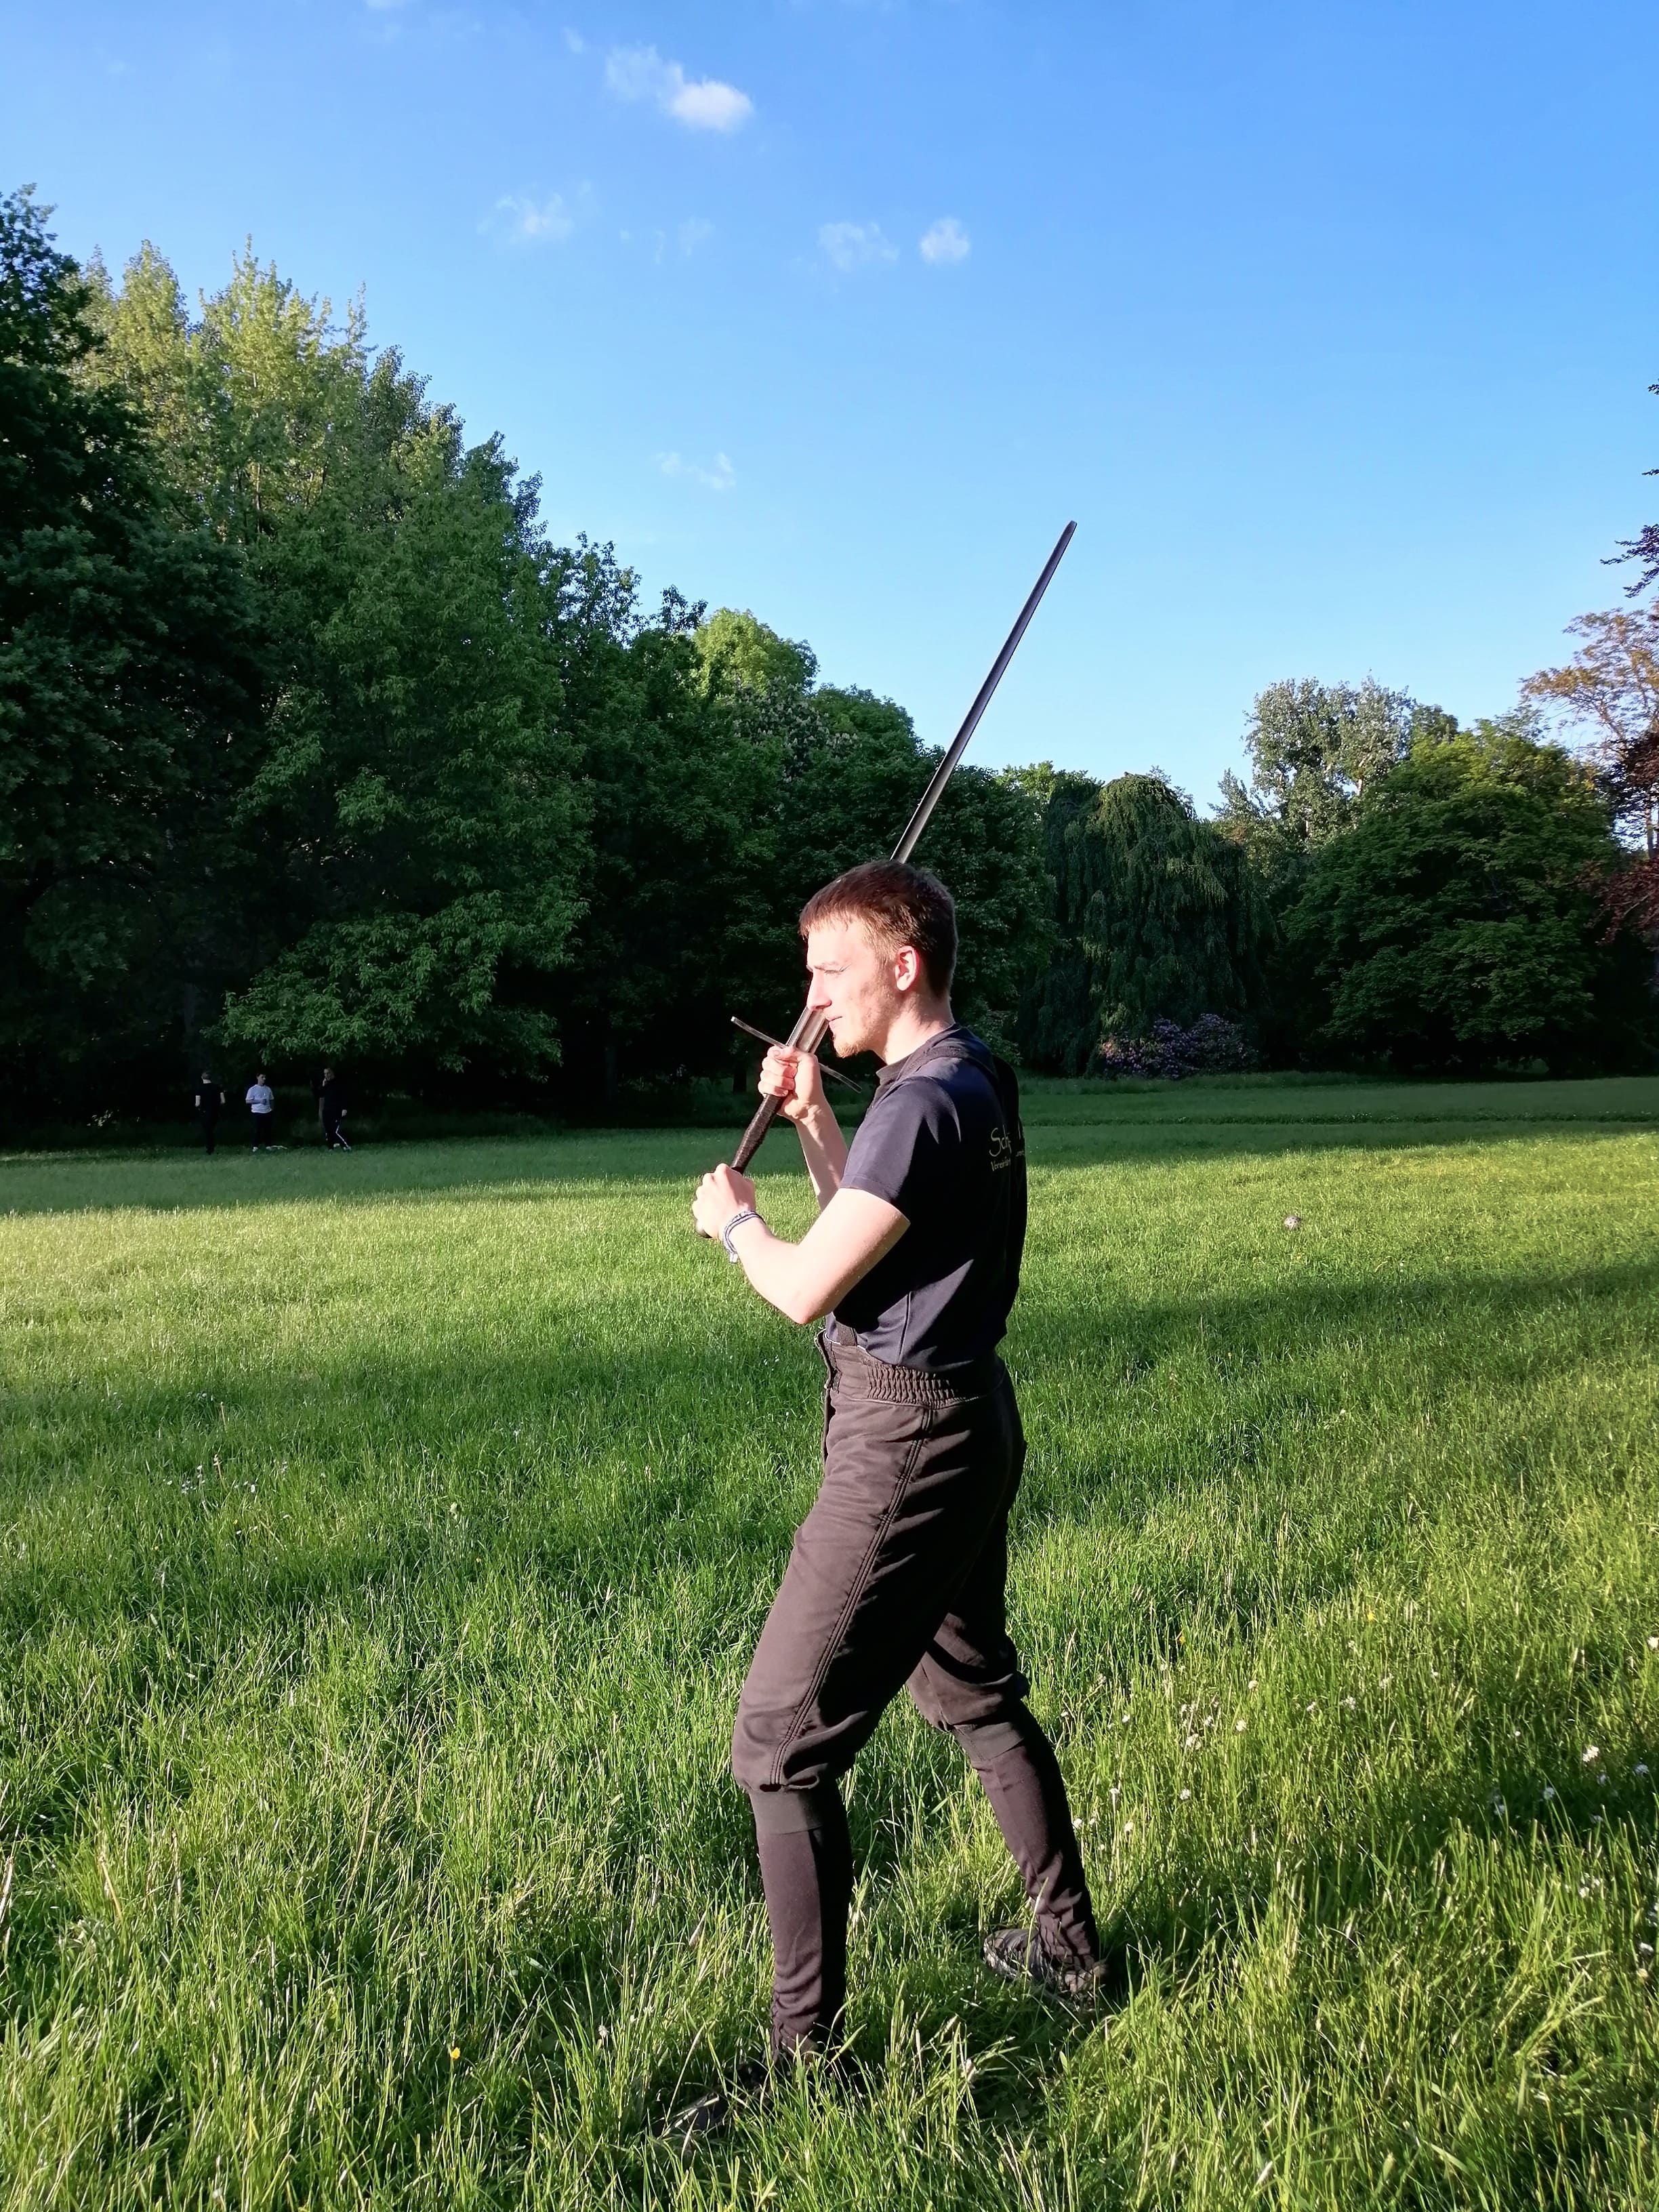
\includegraphics[width=\linewidth]{vonTag1.jpg}
  \caption{links}\label{fig:vt1}
\endminipage\hfill
\minipage{0.32\textwidth}
  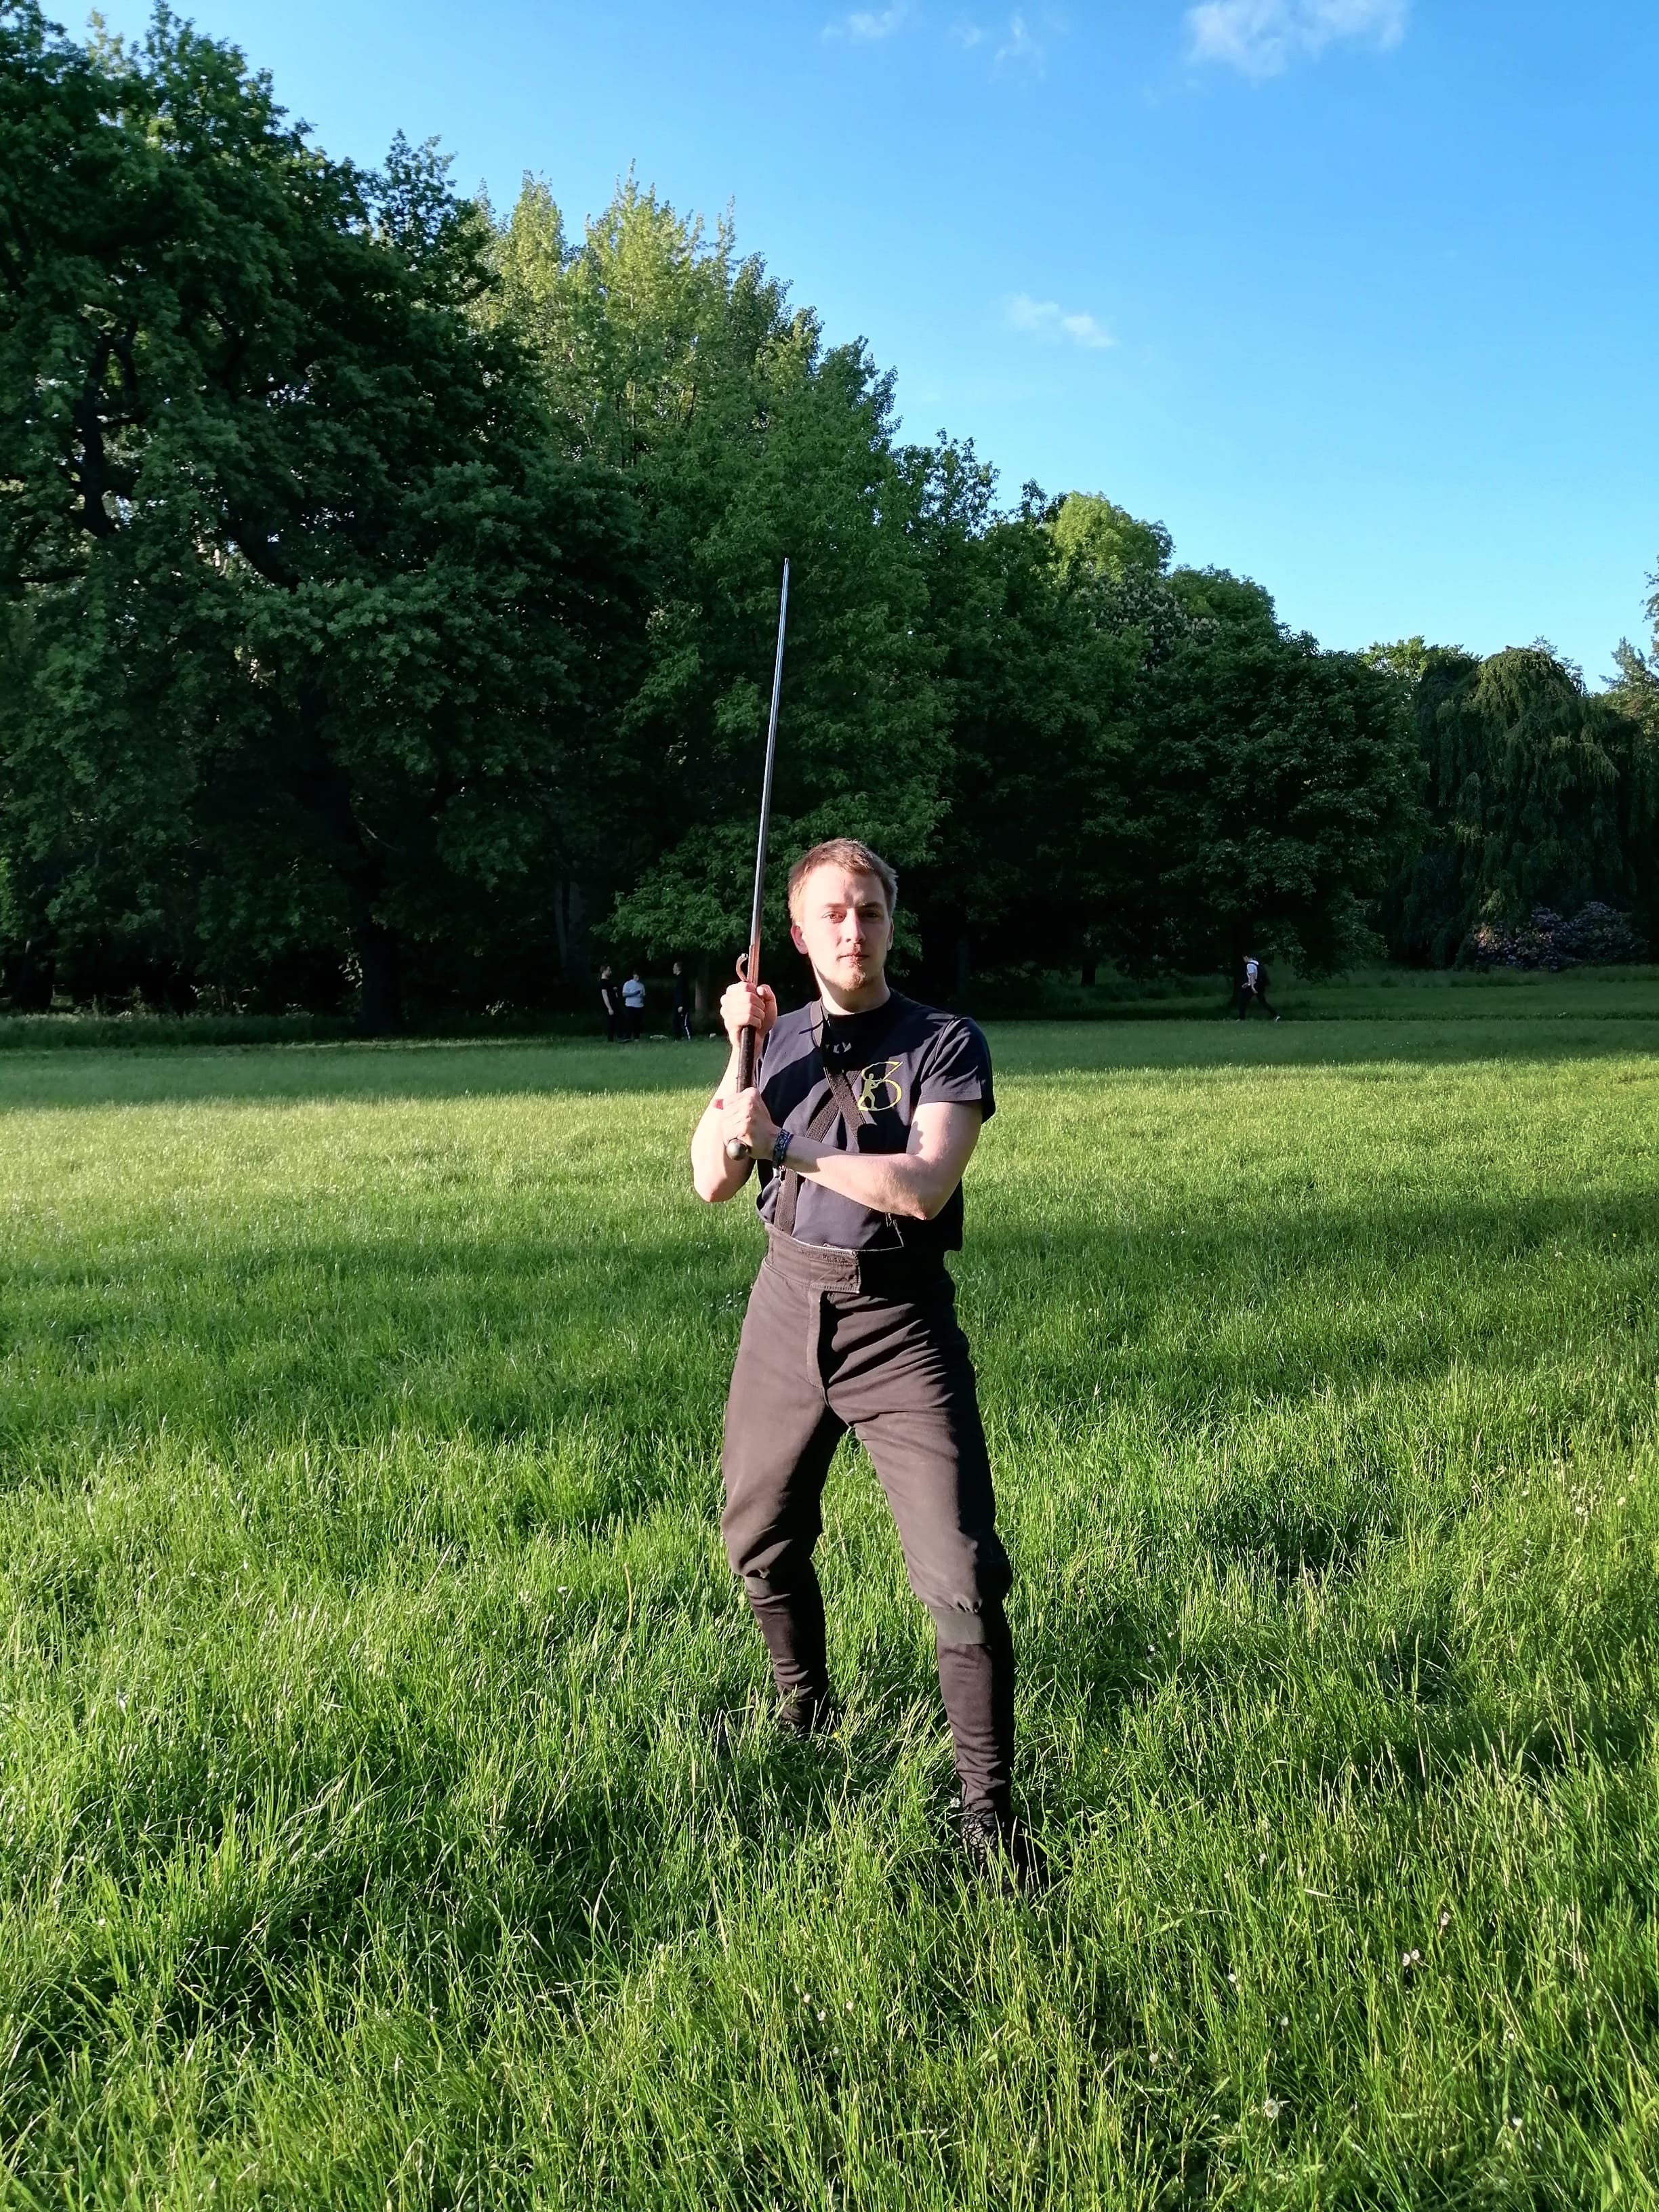
\includegraphics[width=\linewidth]{vonTag2.jpg}
  \caption{frontal}\label{fig:vt2}
\endminipage\hfill
\minipage{0.32\textwidth}%
  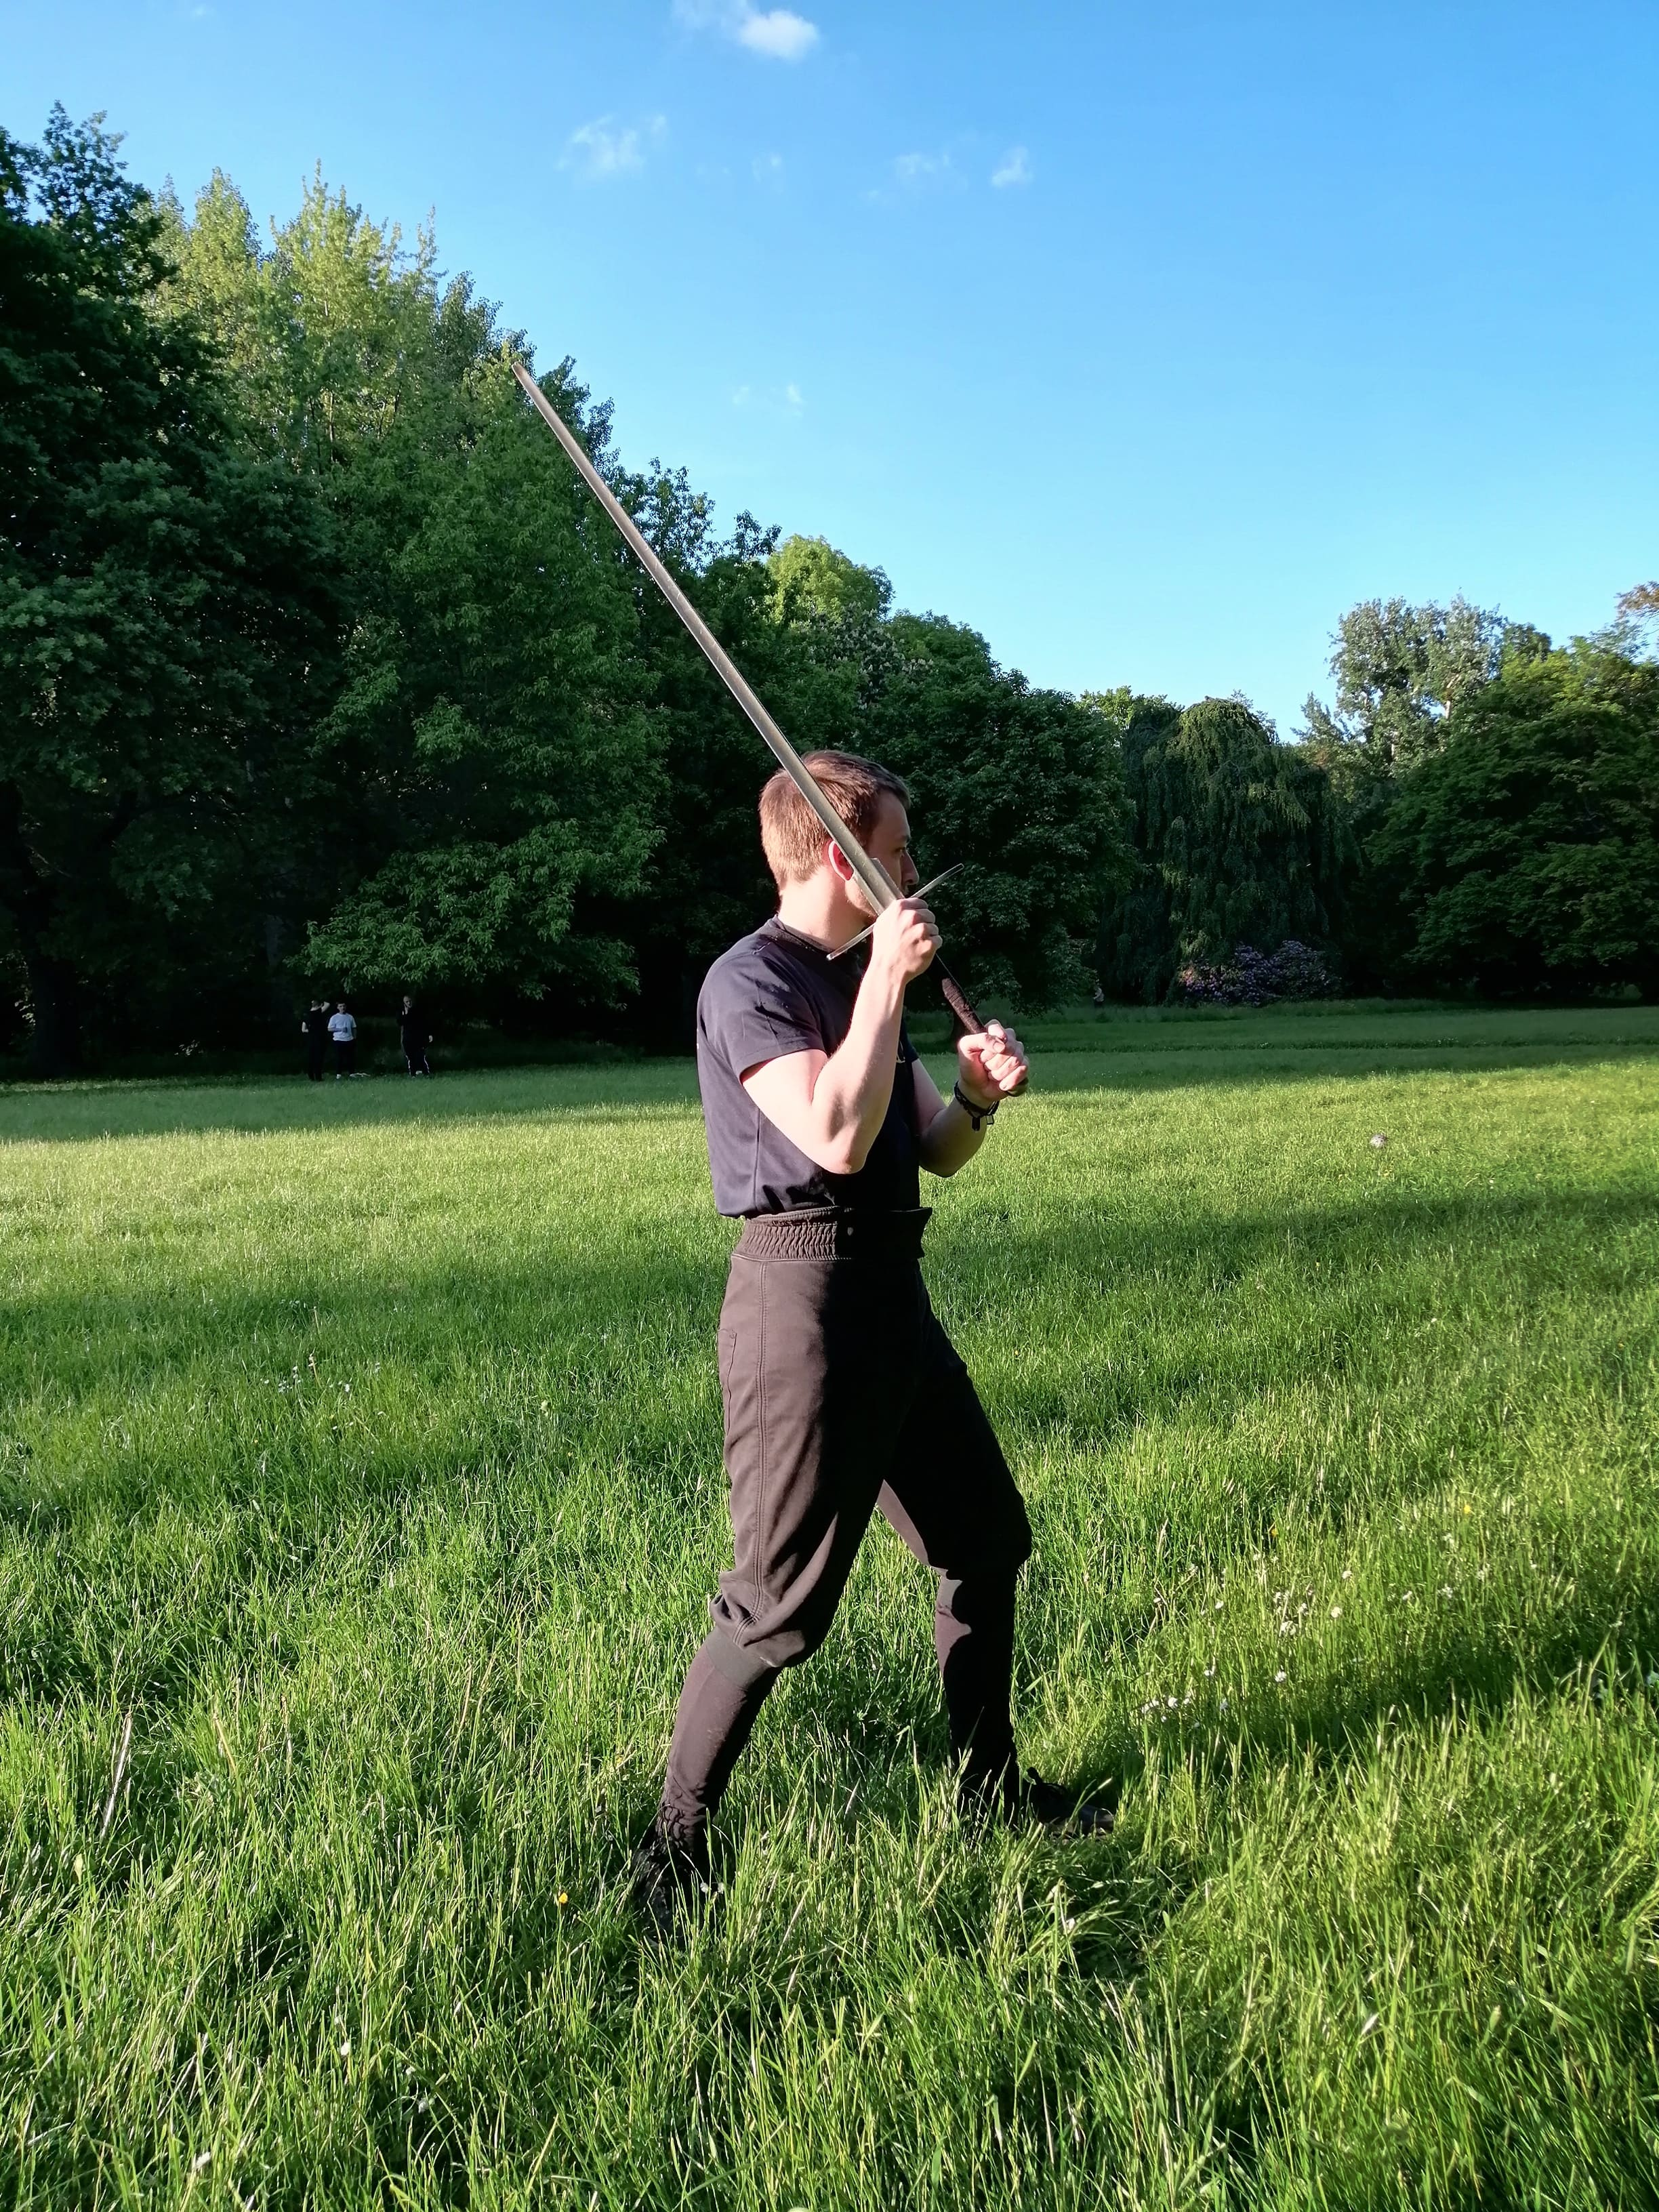
\includegraphics[width=\linewidth]{vonTag3.jpg}
  \caption{rechts}\label{fig:vt3}
\endminipage
\end{figure}

\FloatBarrier

Die Hut ''Vom Tag'' kann in drei Varianten unterteilt werden. Eine neutrale Position wird oft einfach ''Vom Tag'', seltener ''Vom Tag über Kopf'' genannt. Wird das Schwert auf einer Seite gehalten, fügt man dieser Seite den Namen hinzu ''Vom Tag, (Schulter) rechts / links''. Beide Seiten werden identisch ausgeführt, jedoch gespiegelt. Das Schwert wird vorzugsweise im Hammergriff gehalten.
\\
\hrule

\paragraph{Pflug}

\begin{figure}[ht!]
\minipage{0.32\textwidth}
  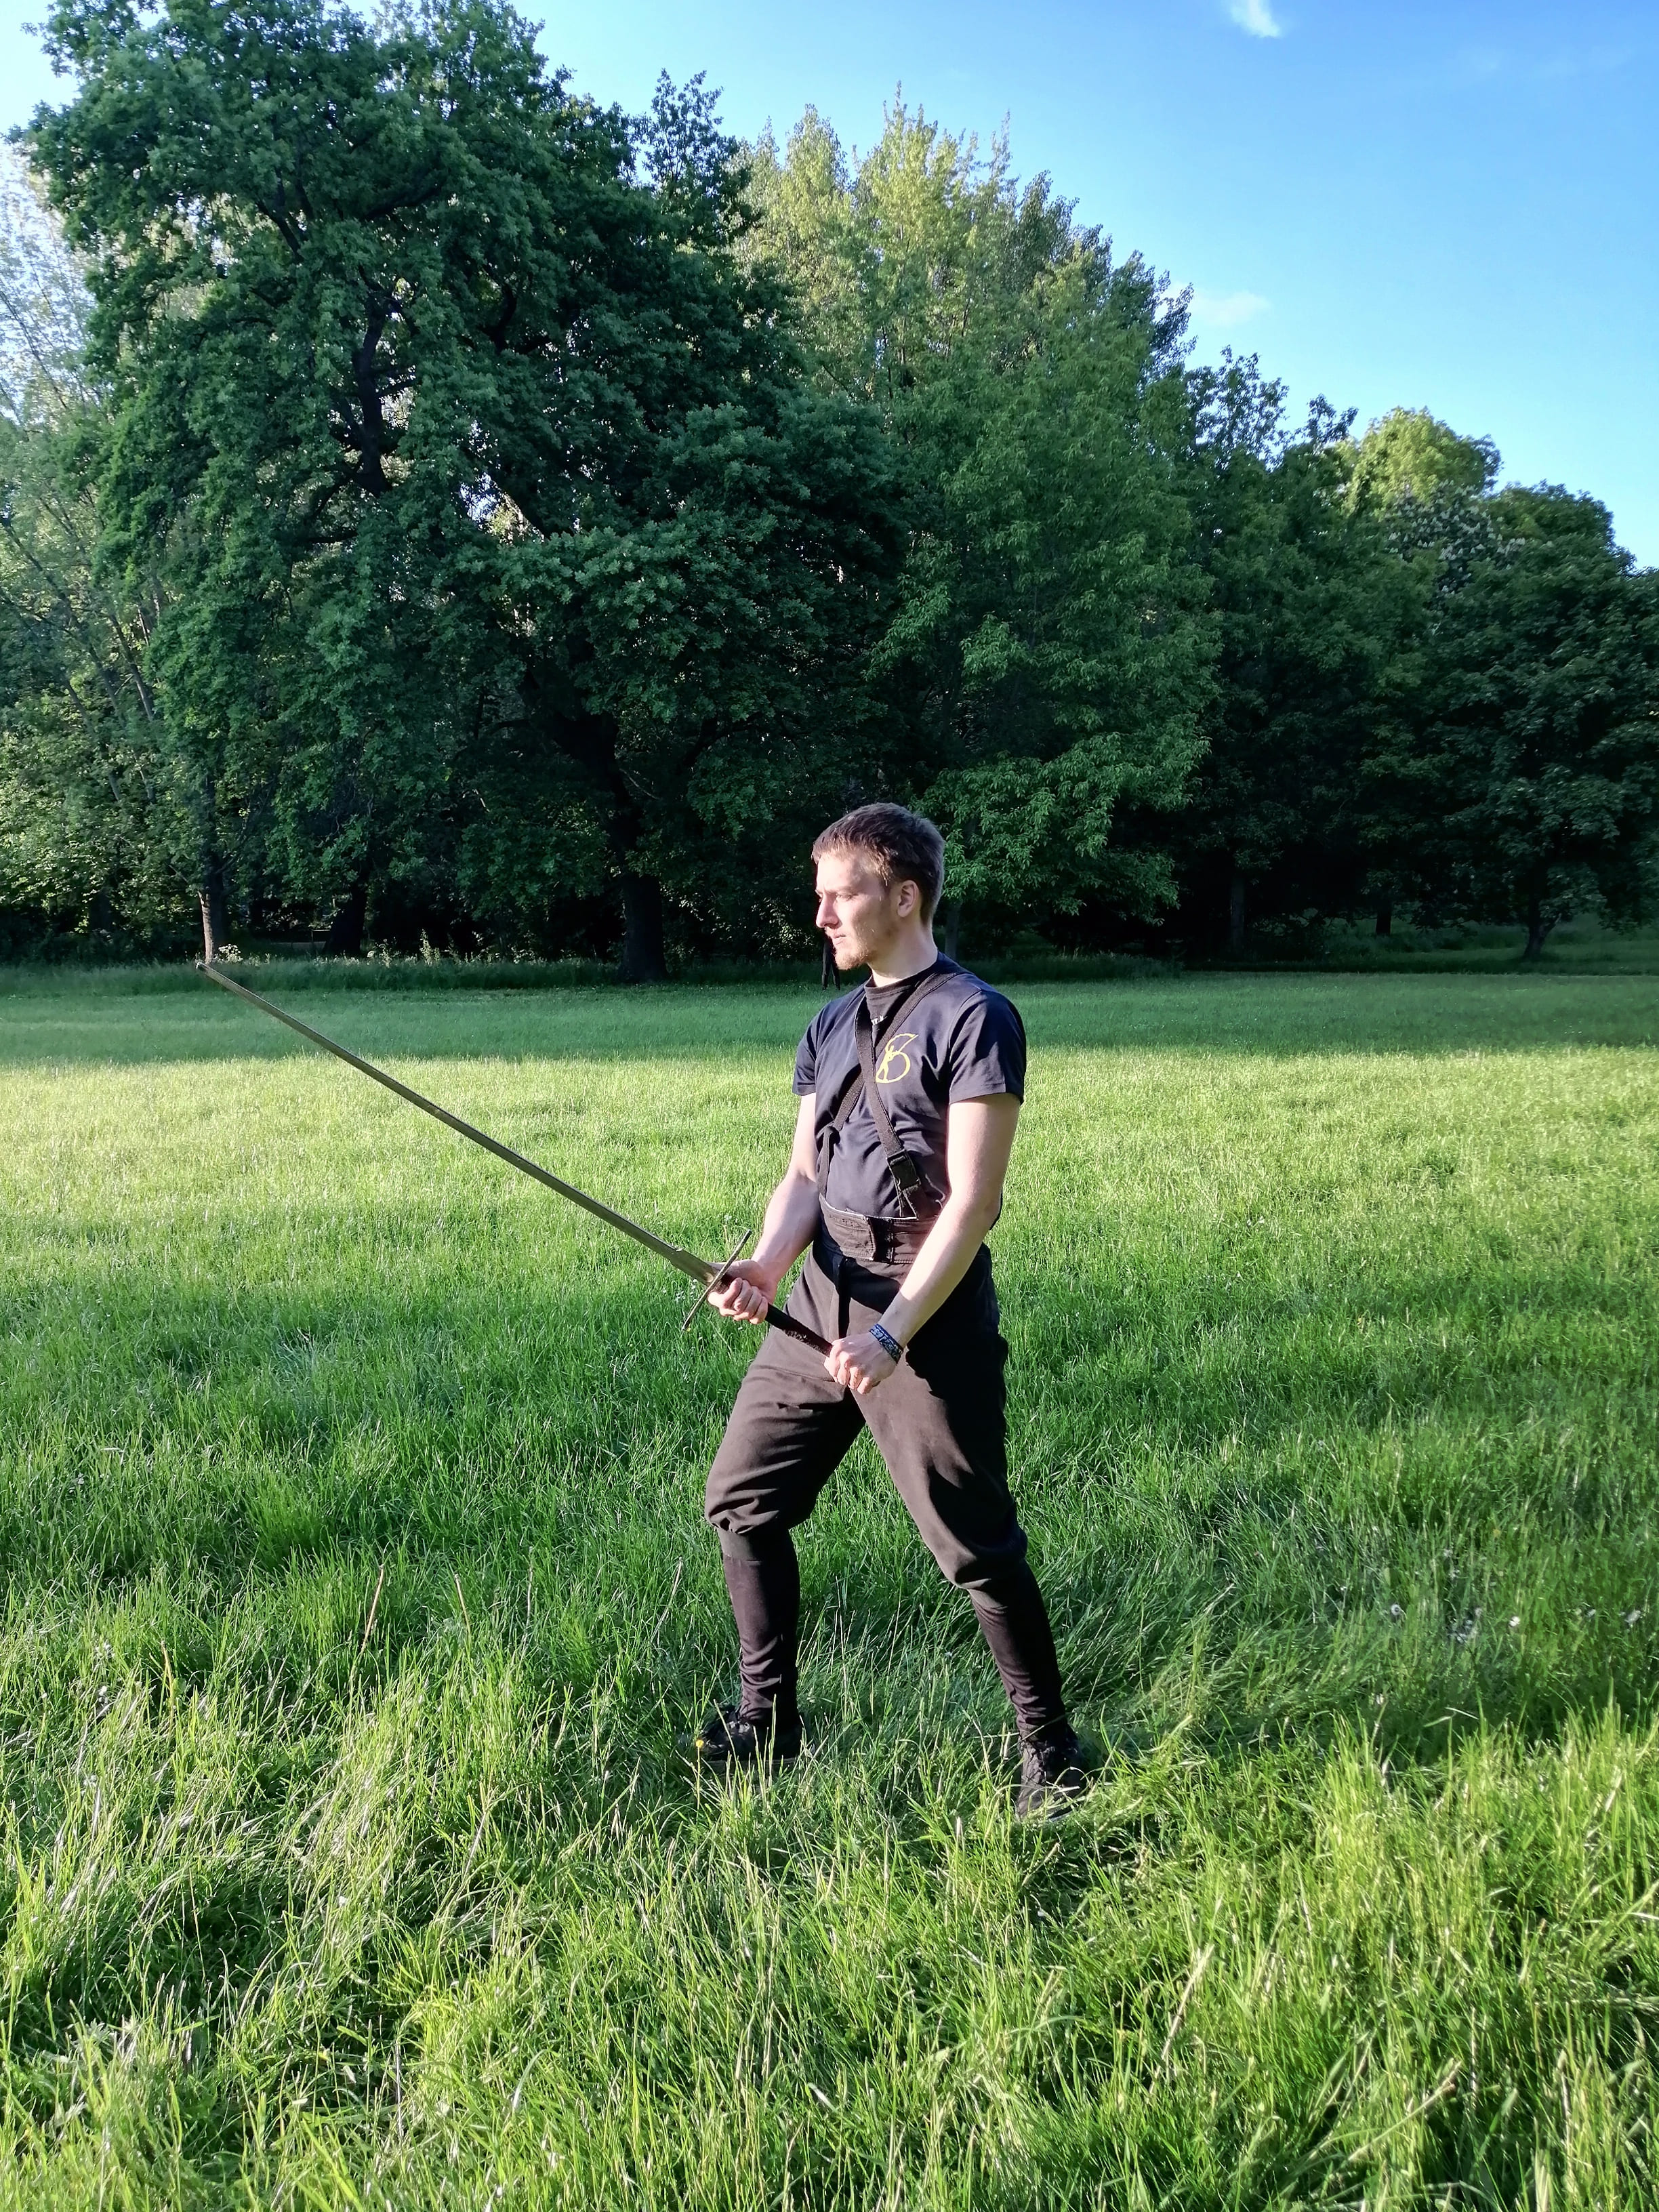
\includegraphics[width=\linewidth]{Pflug1.jpg}
  \caption{links}\label{fig:pflug1}
\endminipage\hfill
\minipage{0.32\textwidth}
  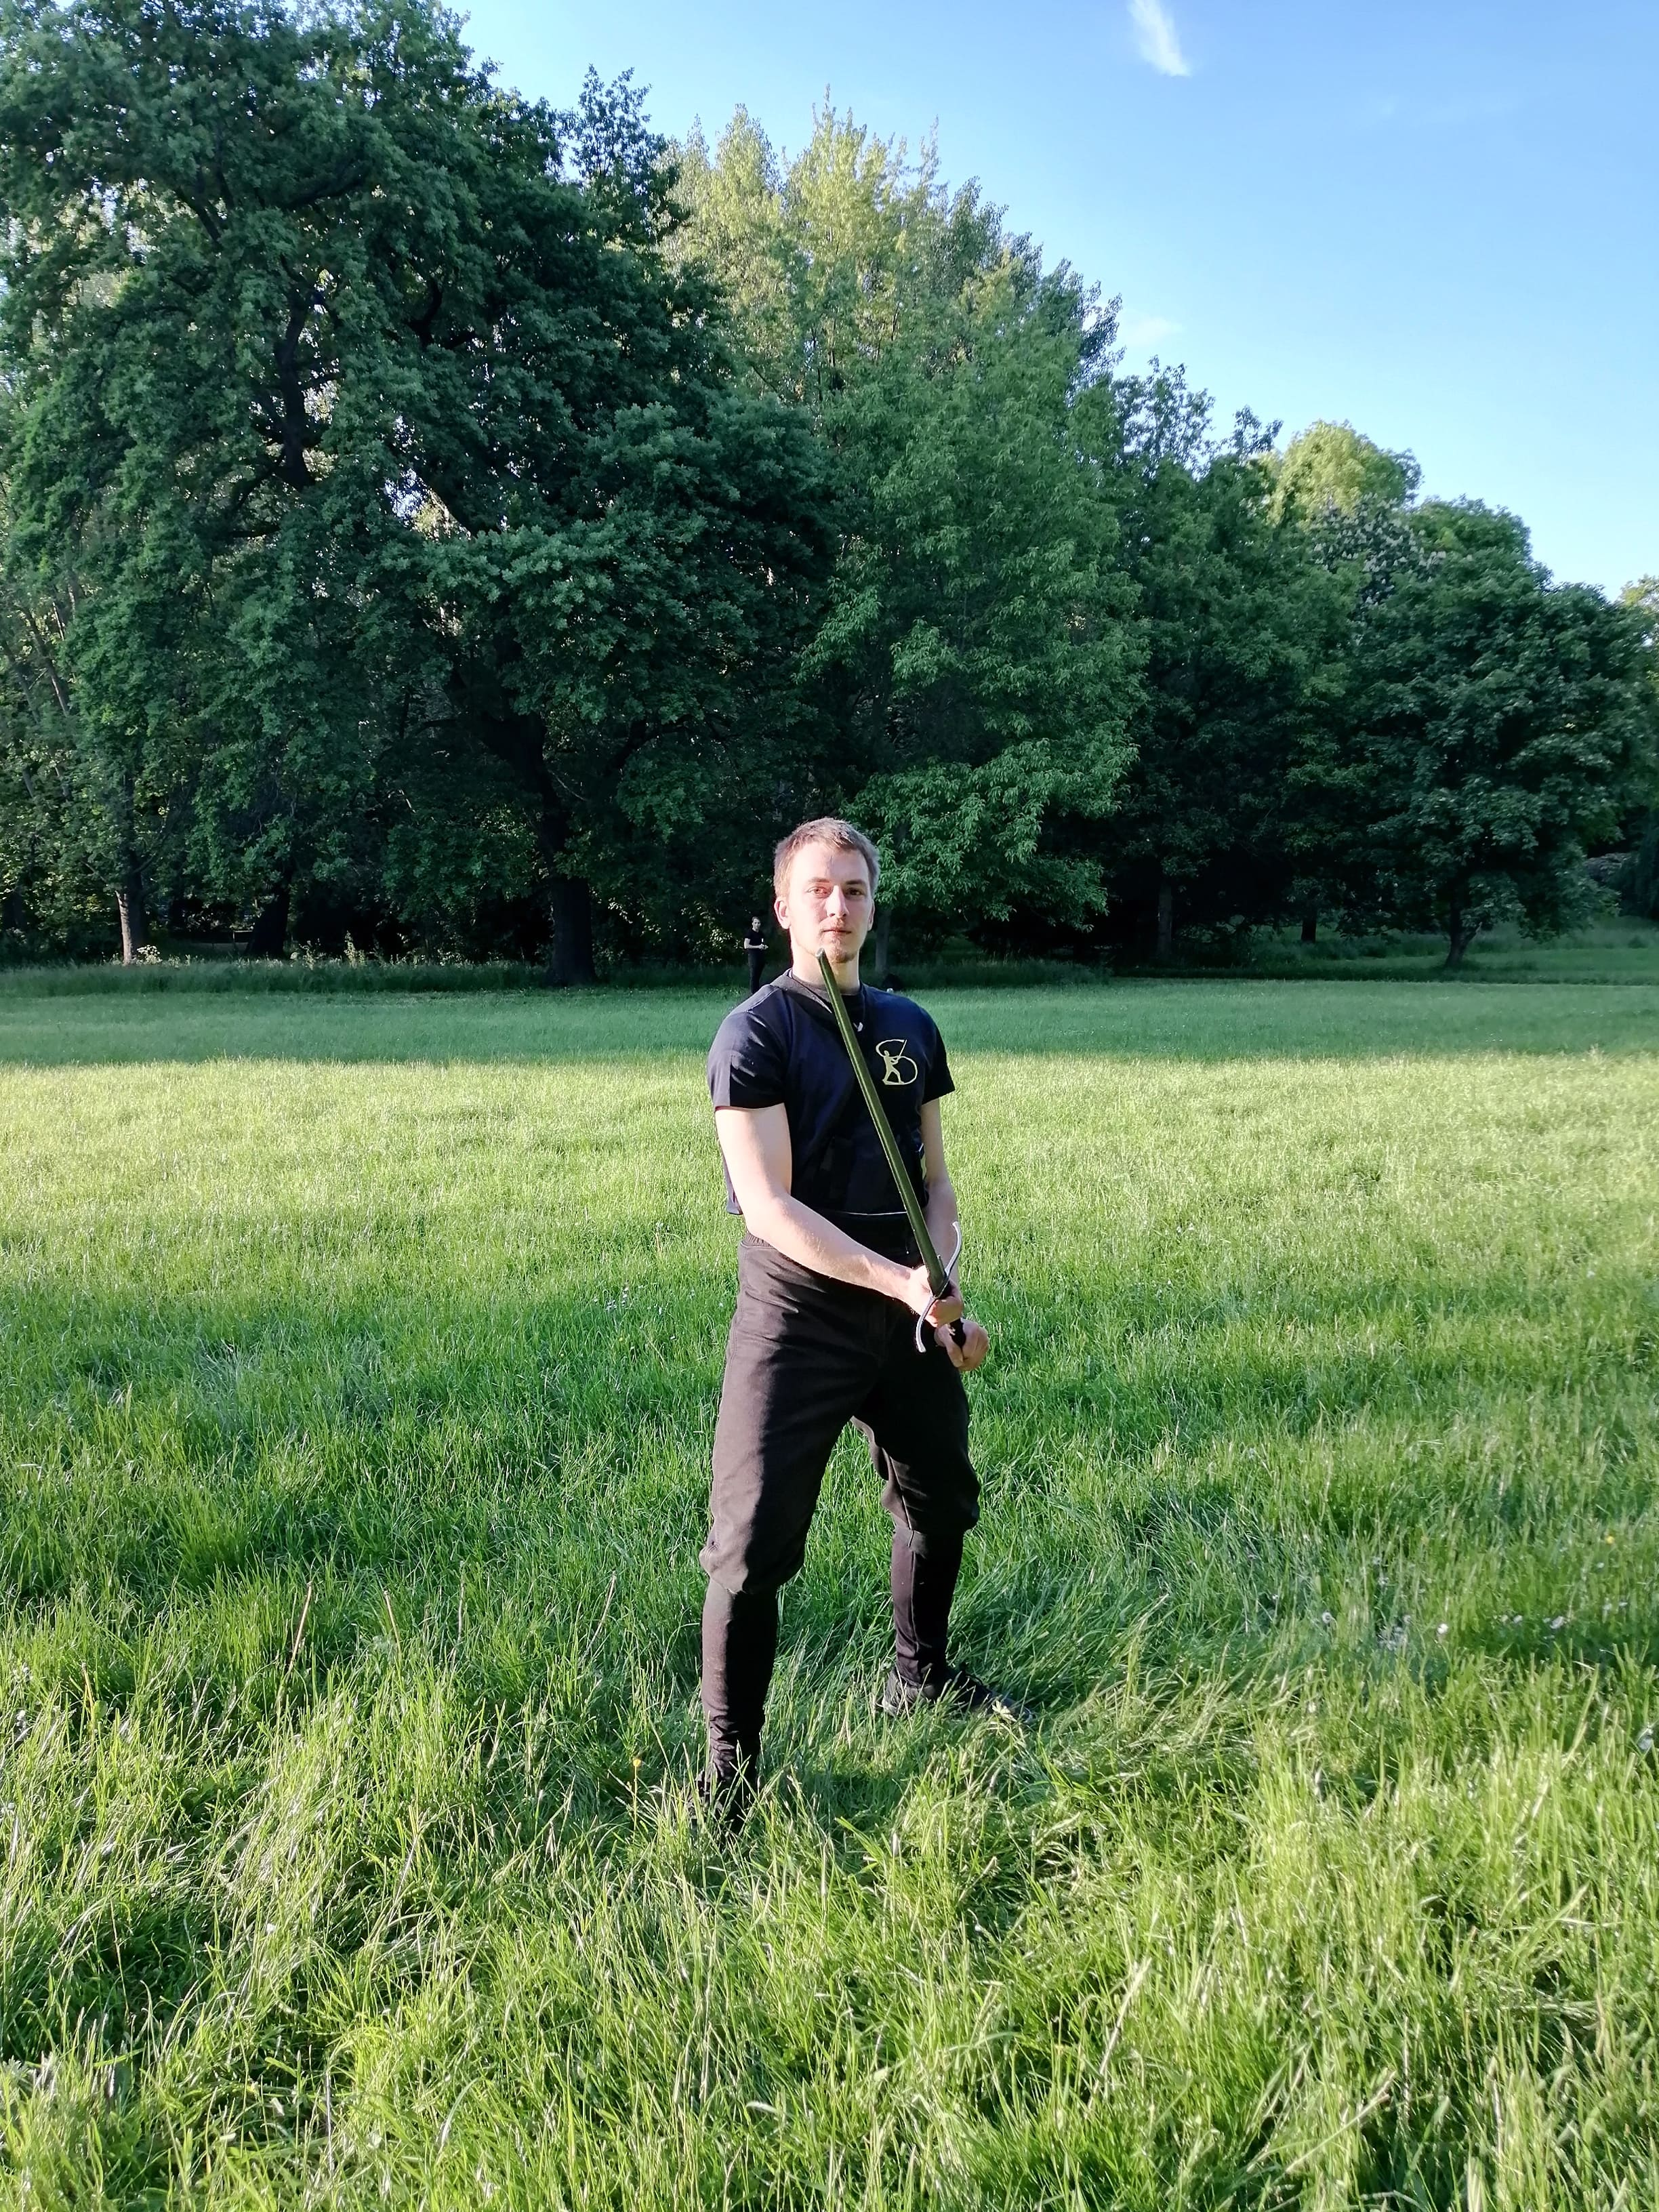
\includegraphics[width=\linewidth]{Pflug2.jpg}
  \caption{frontal}\label{fig:pflug2}
\endminipage\hfill
\minipage{0.32\textwidth}%
  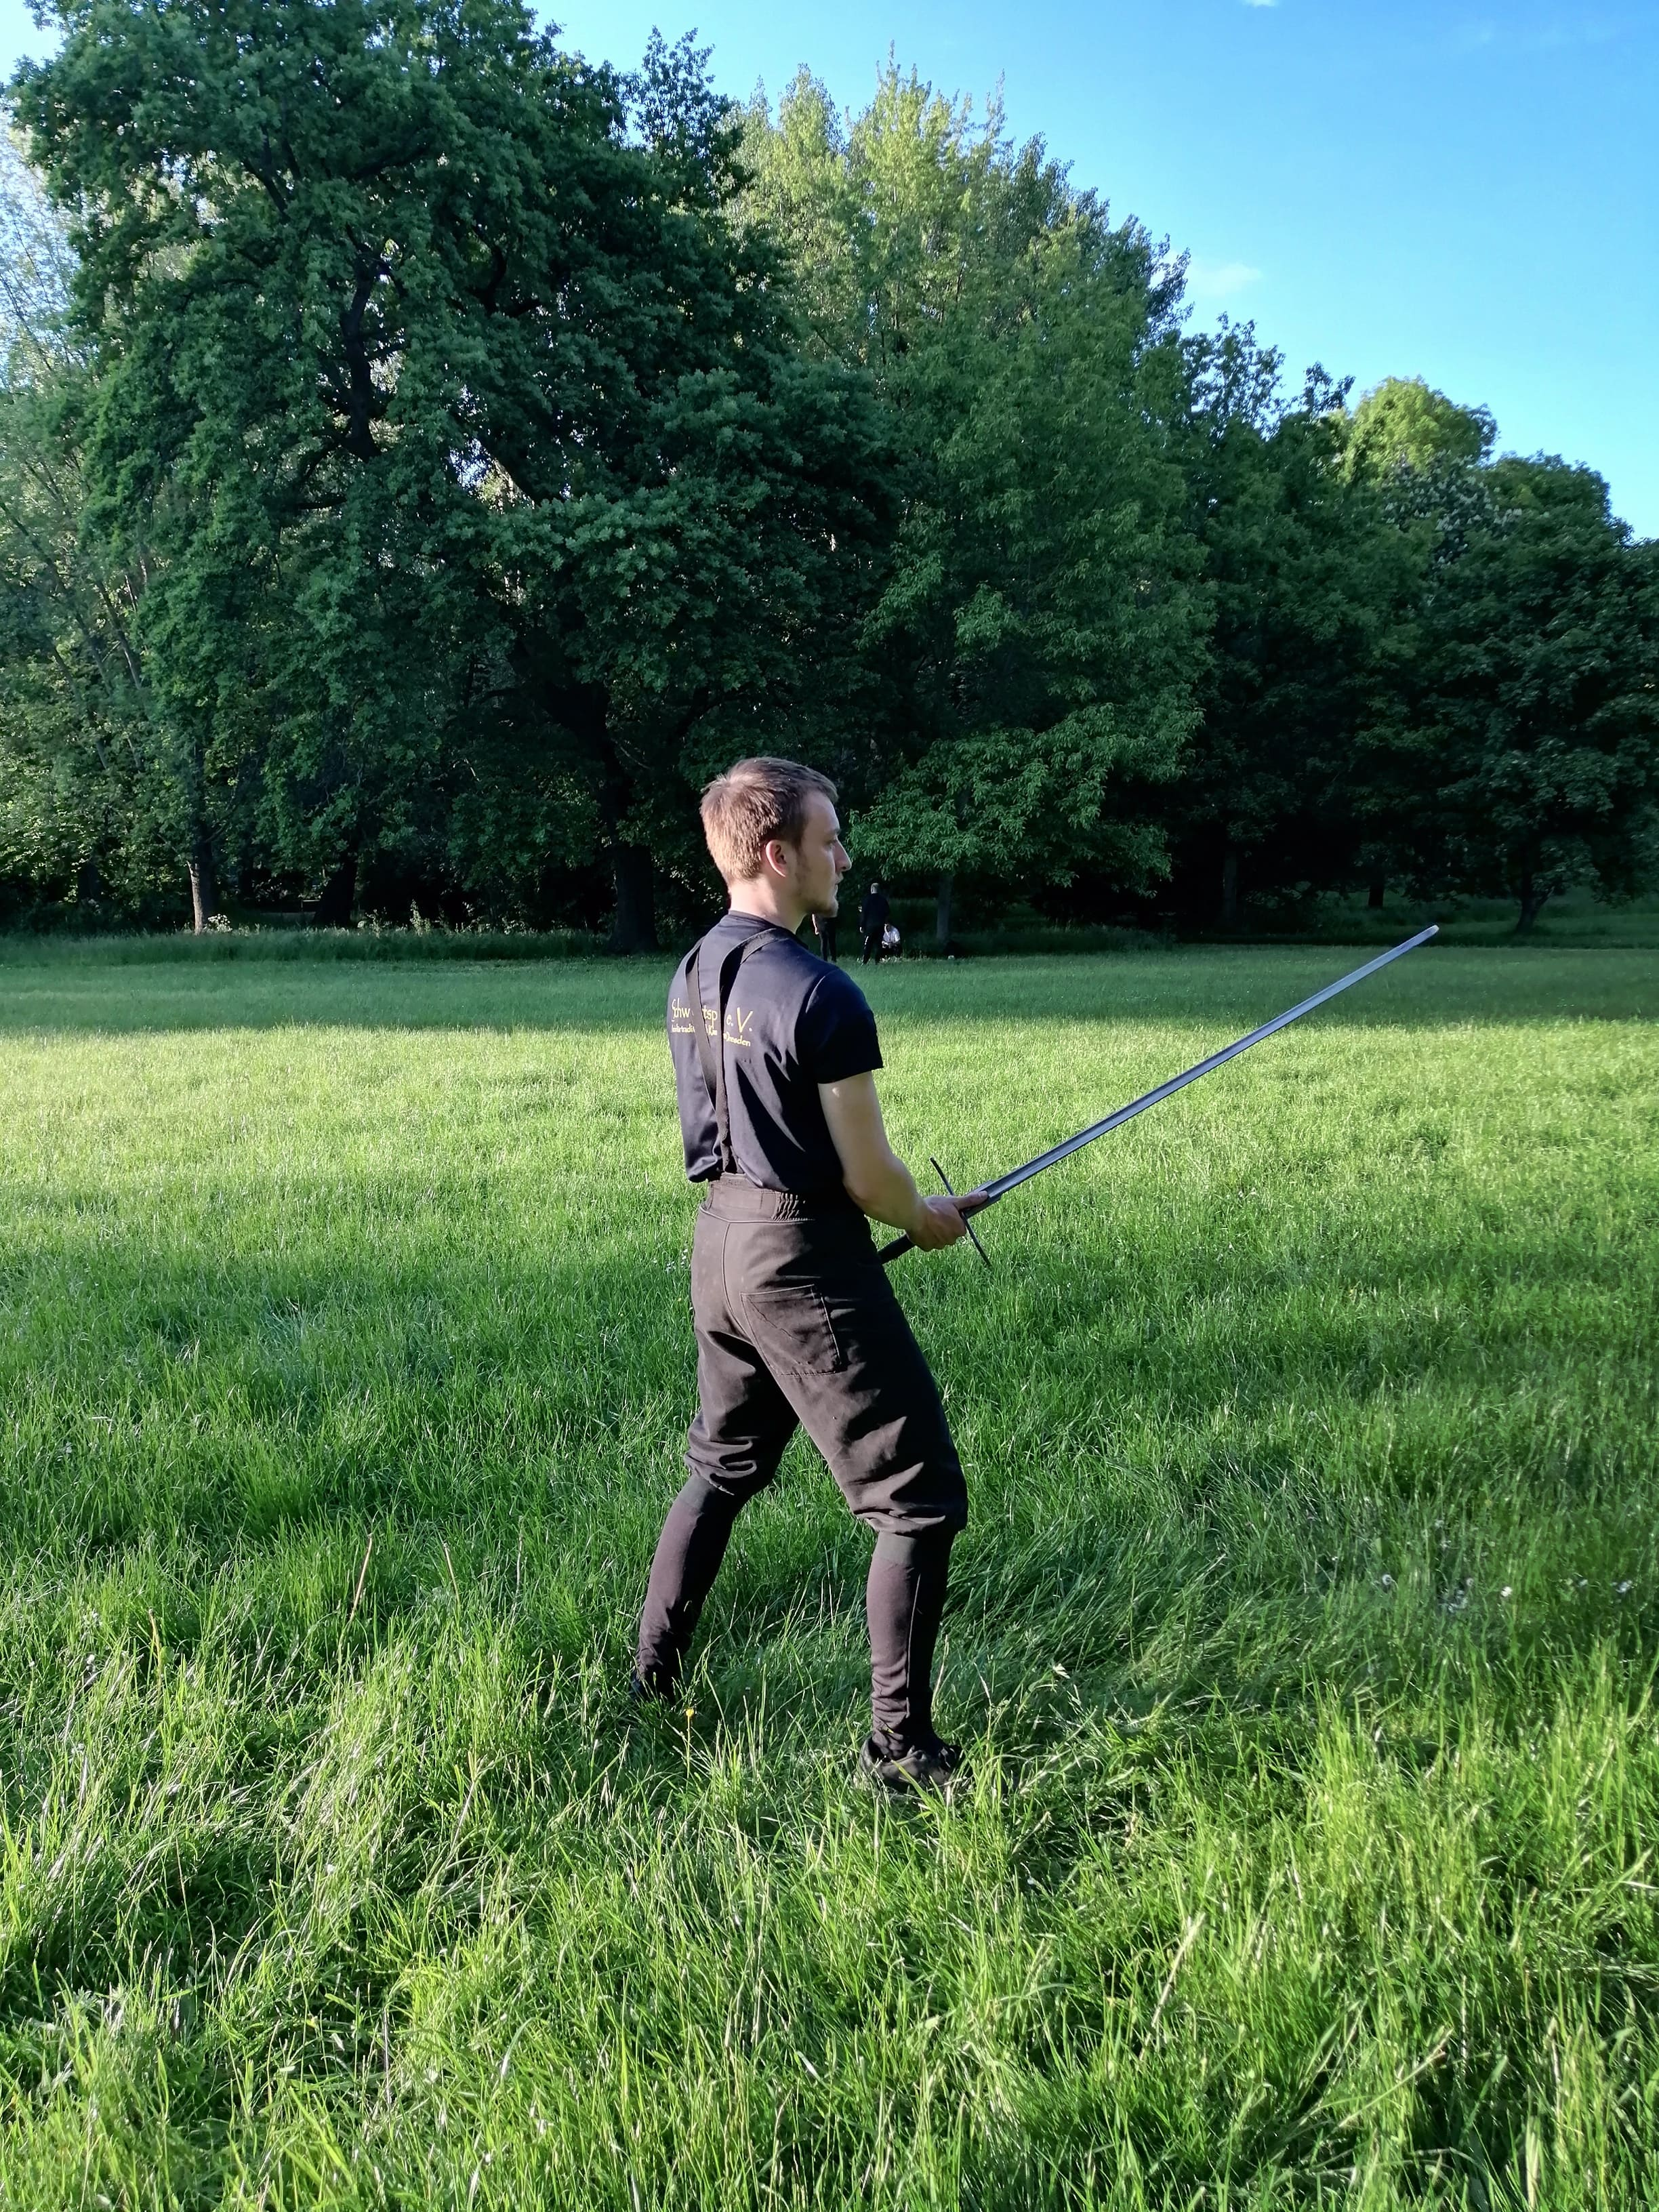
\includegraphics[width=\linewidth]{Pflug3.jpg}
  \caption{rechts}\label{fig:pflug3}
\endminipage
\end{figure}

\FloatBarrier

Die Hut ''Plfug'' wird ebenfalls in links und rechts unterschieden. Beide Seiten werden identisch ausgeführt, jedoch gespiegelt. Das Schwert wird oft im Daumengriff gehalten.

\clearpage

\paragraph{Ochs}

\begin{figure}[h!t]
\minipage{0.32\textwidth}
  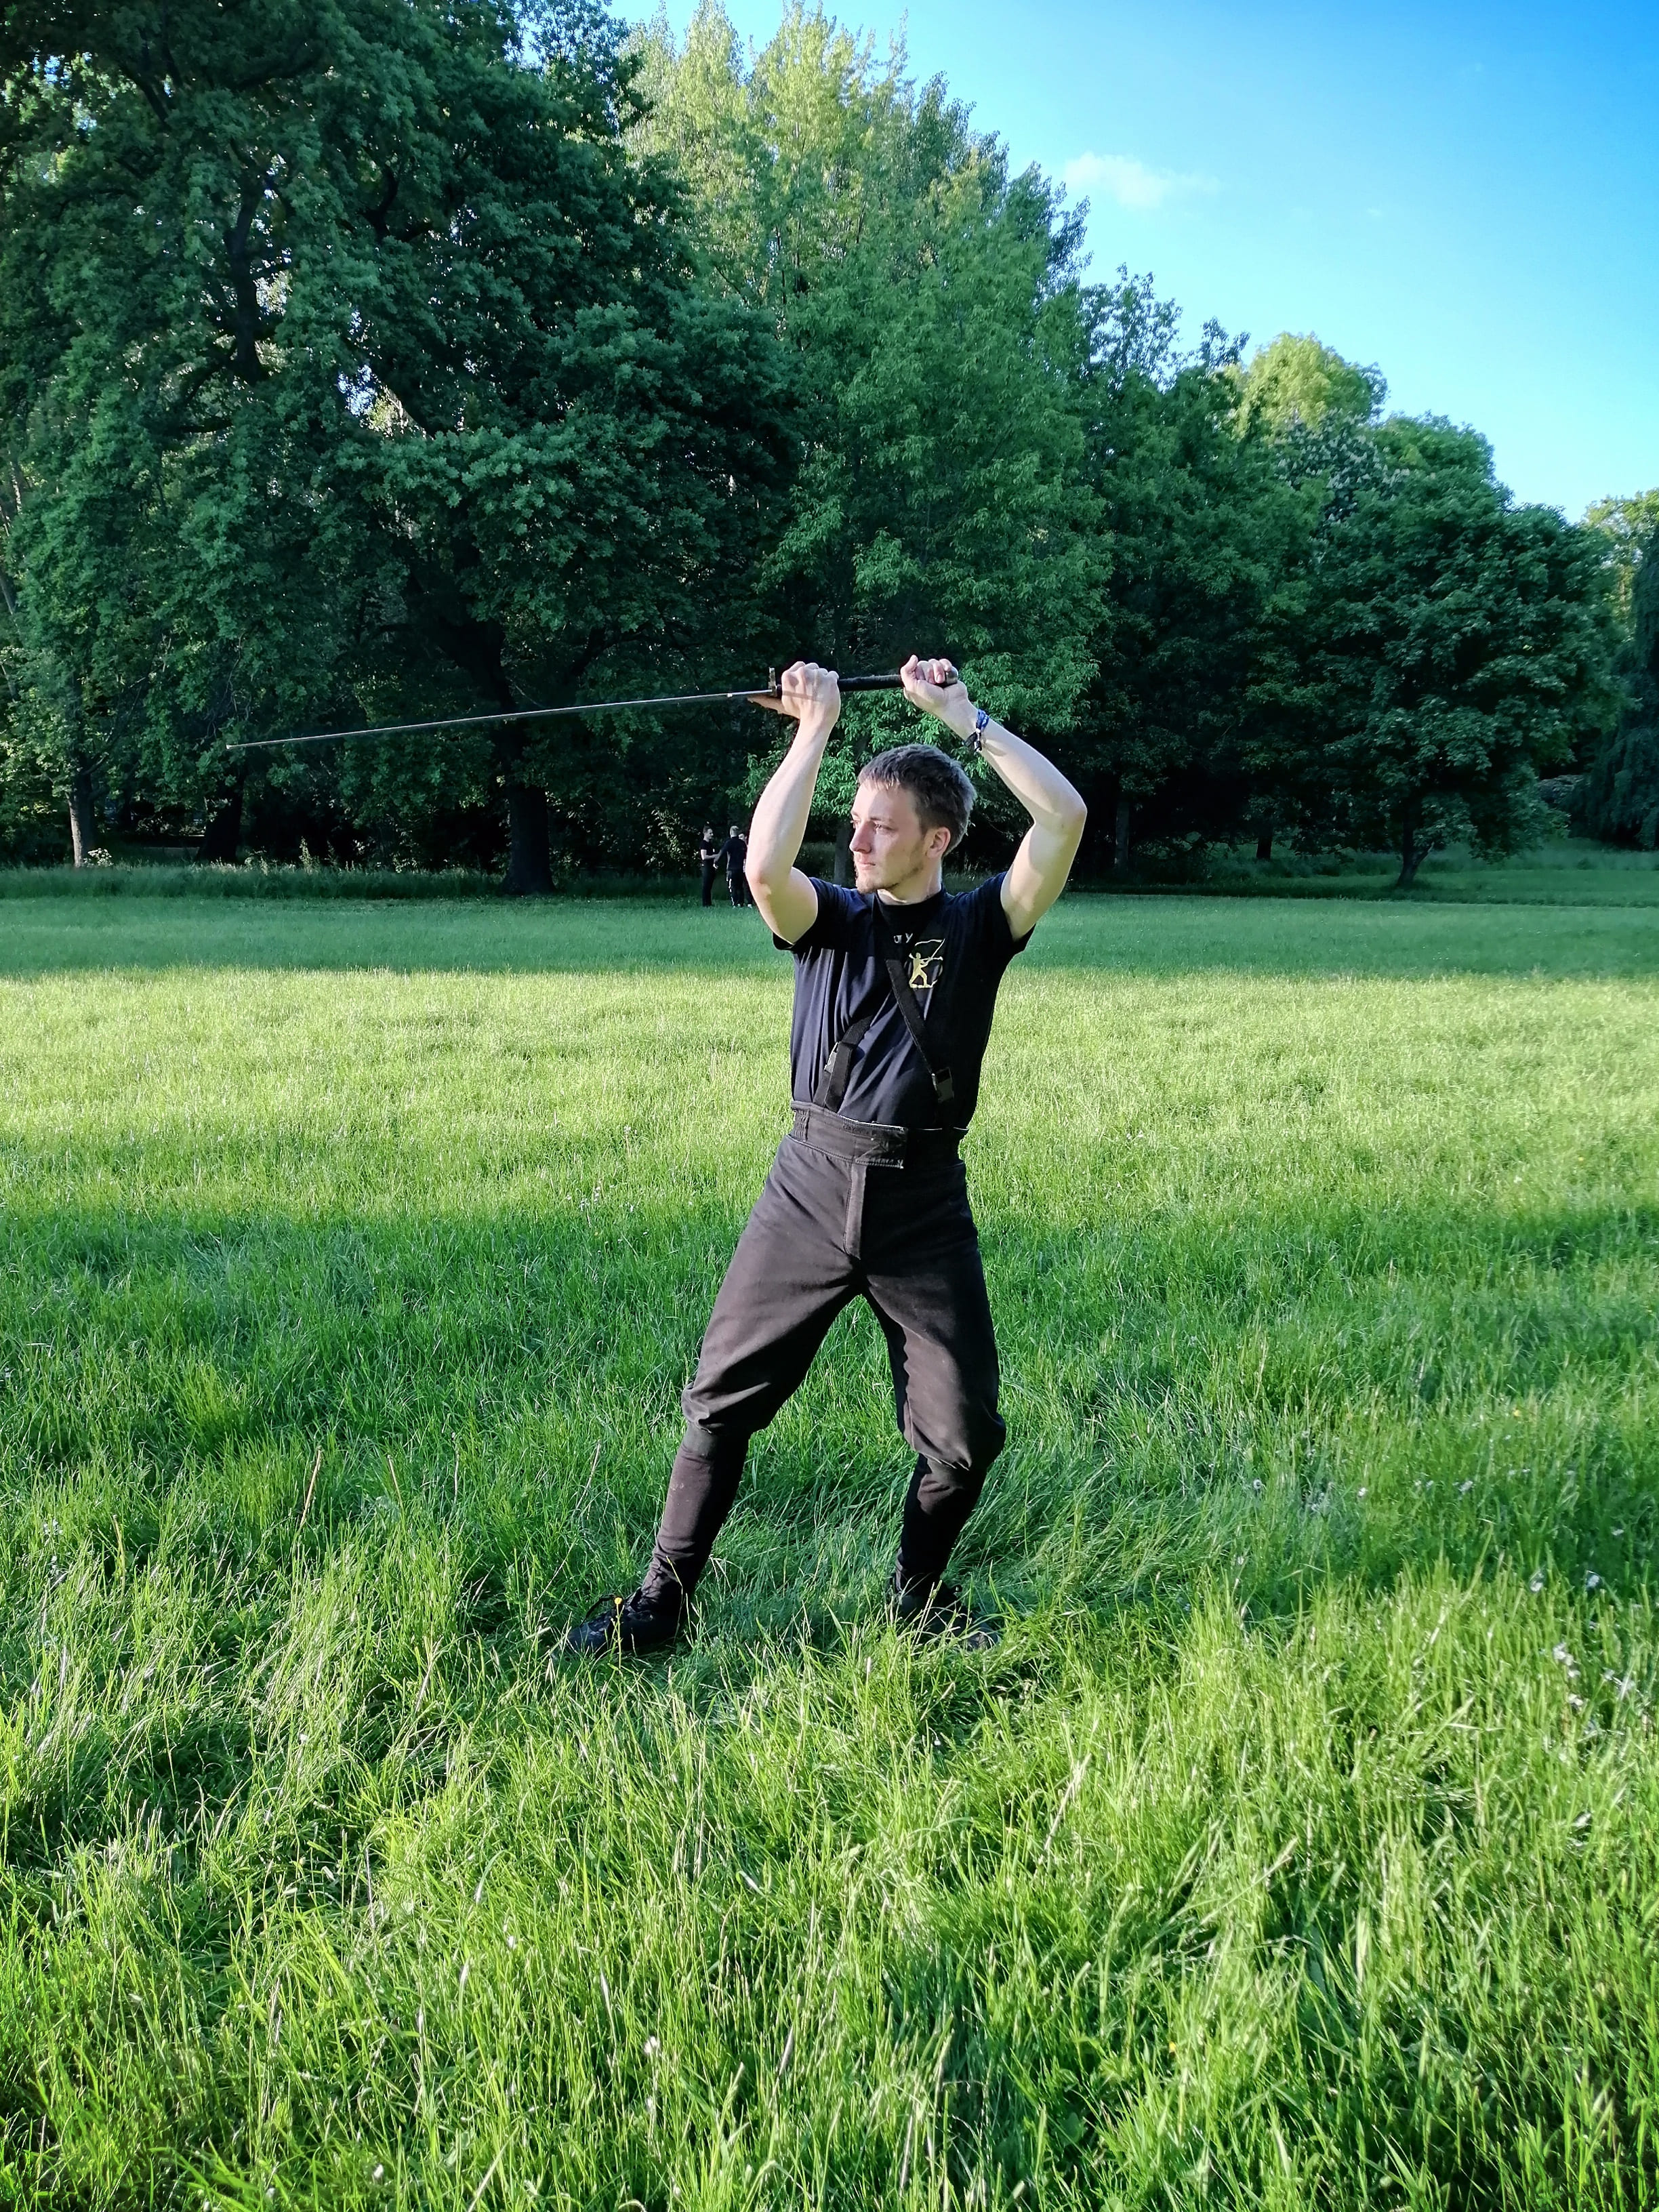
\includegraphics[width=\linewidth]{Ochs1.jpg}
  \caption{Ochs links}\label{fig:ochs1}
\endminipage\hfill
\minipage{0.32\textwidth}
  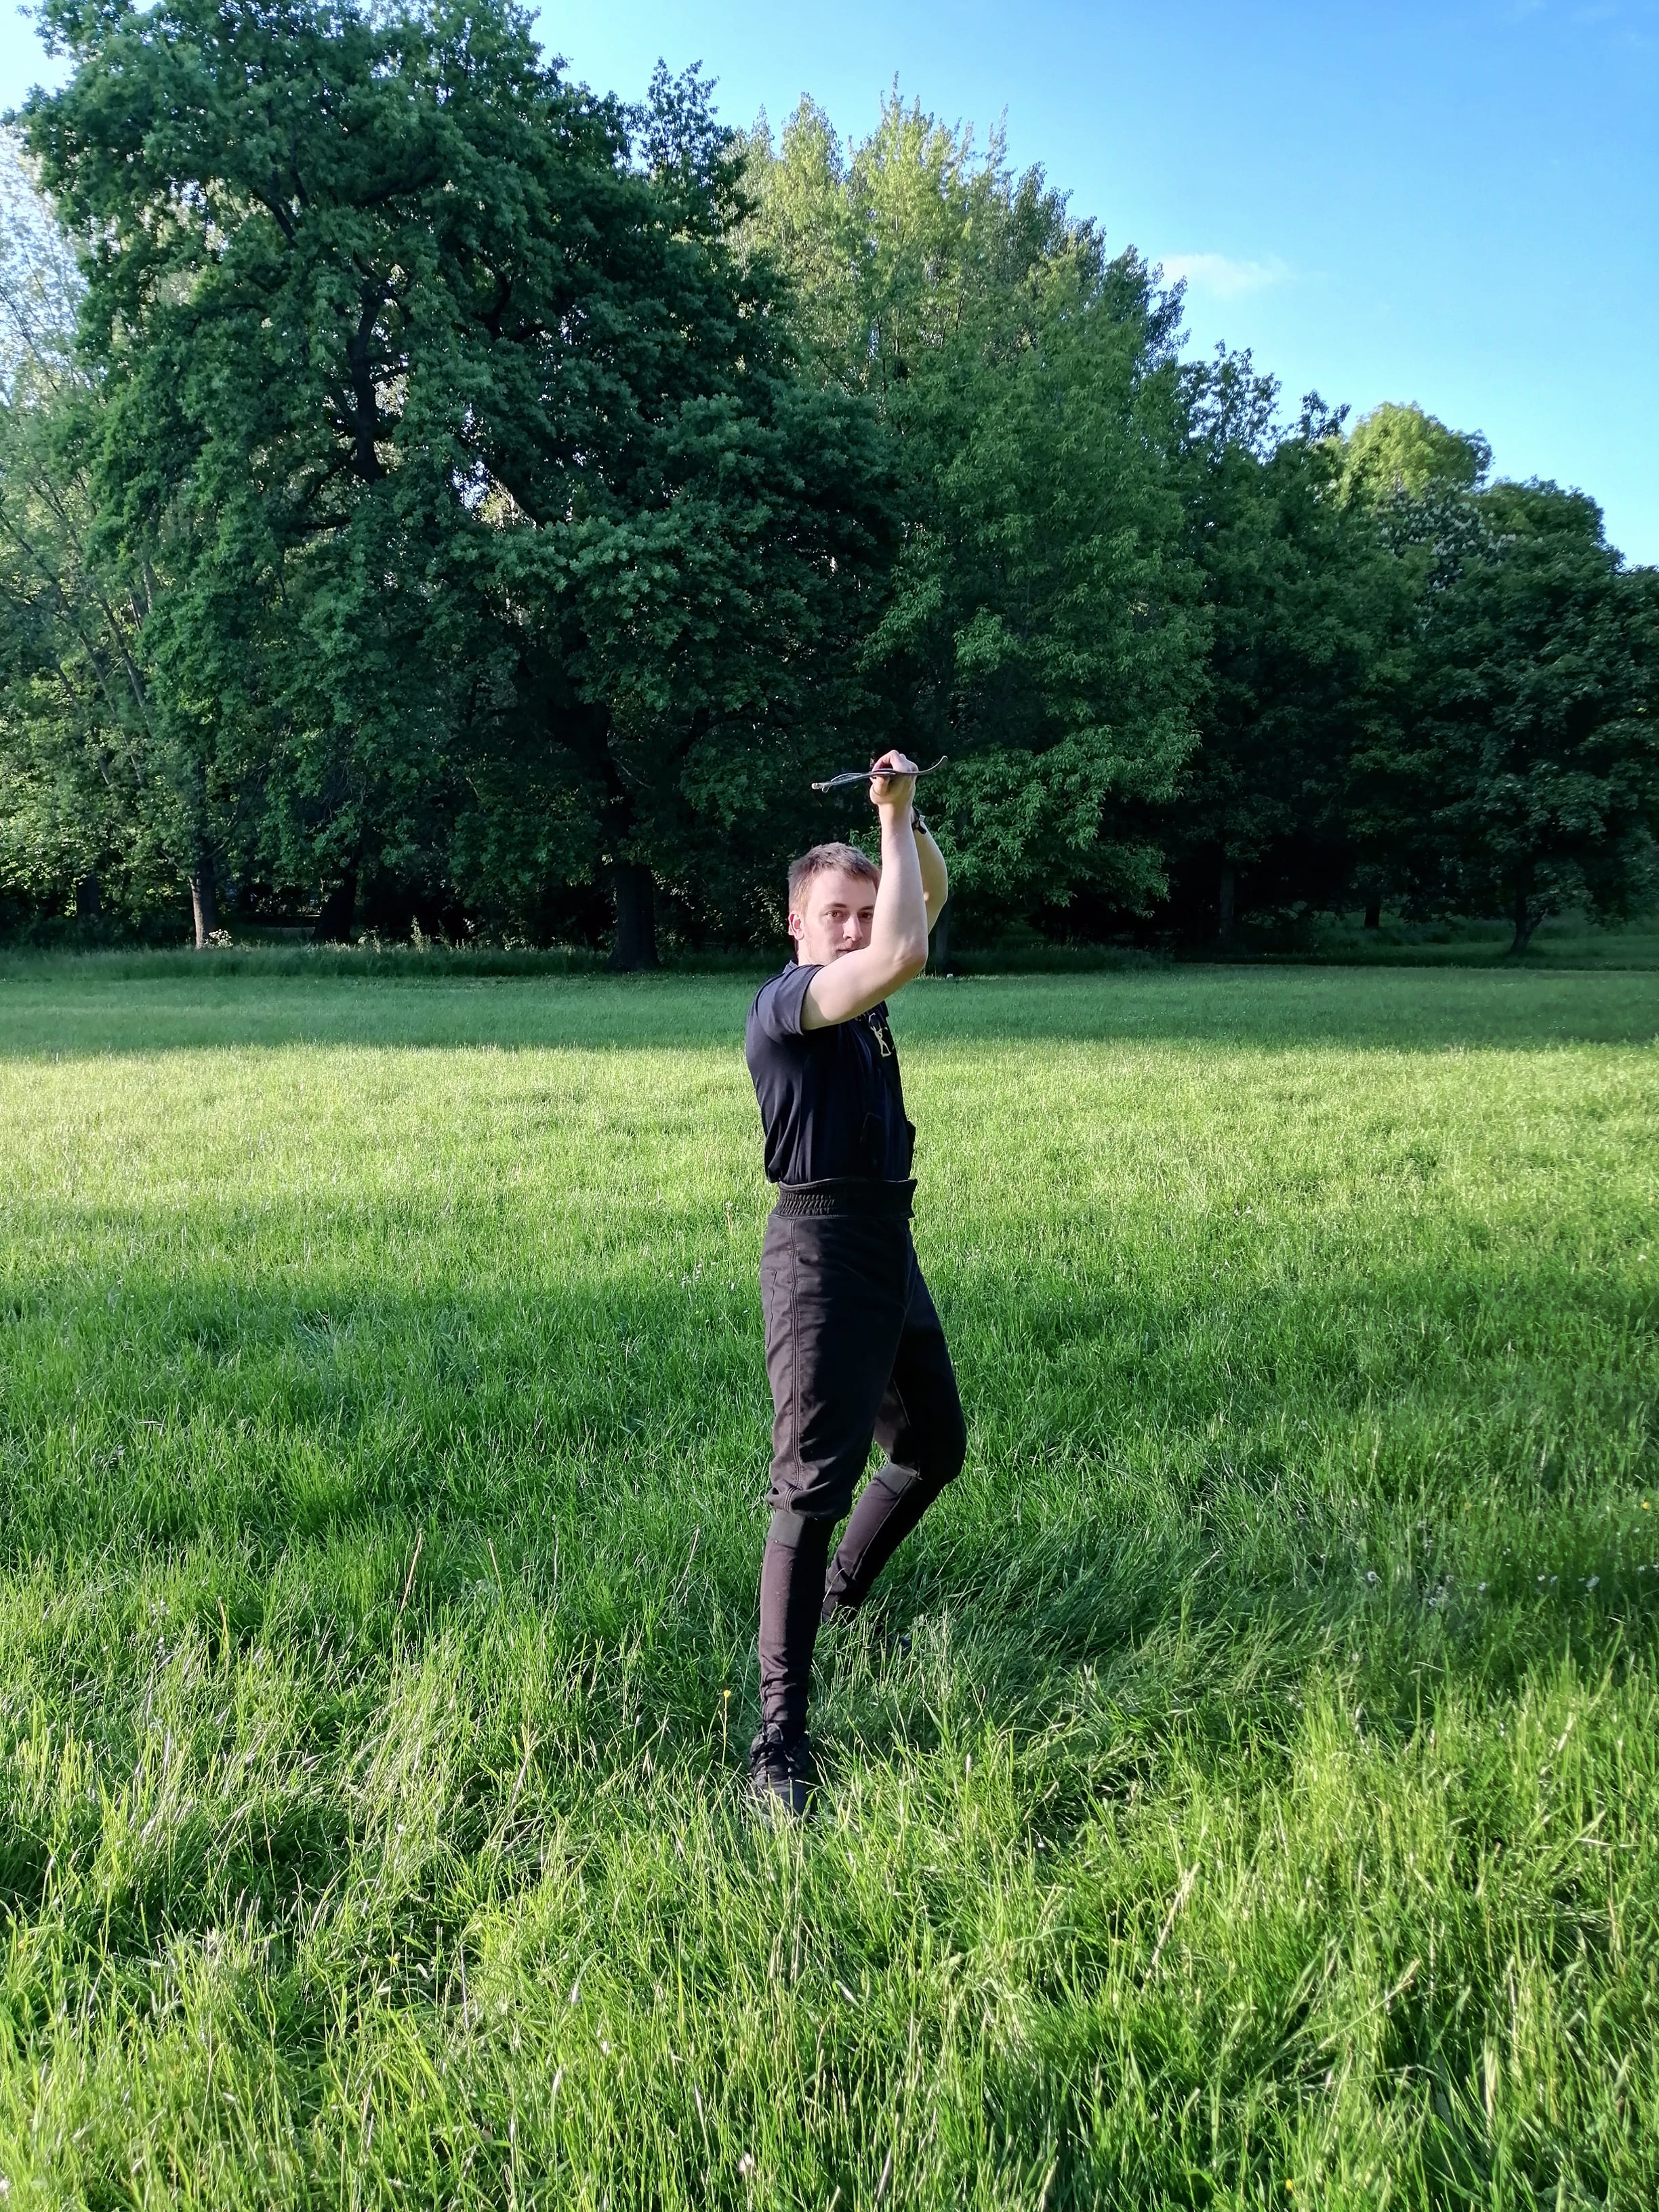
\includegraphics[width=\linewidth]{Ochs2.jpg}
  \caption{Ochs links}\label{fig:ochs2}
\endminipage\hfill
\minipage{0.32\textwidth}%
  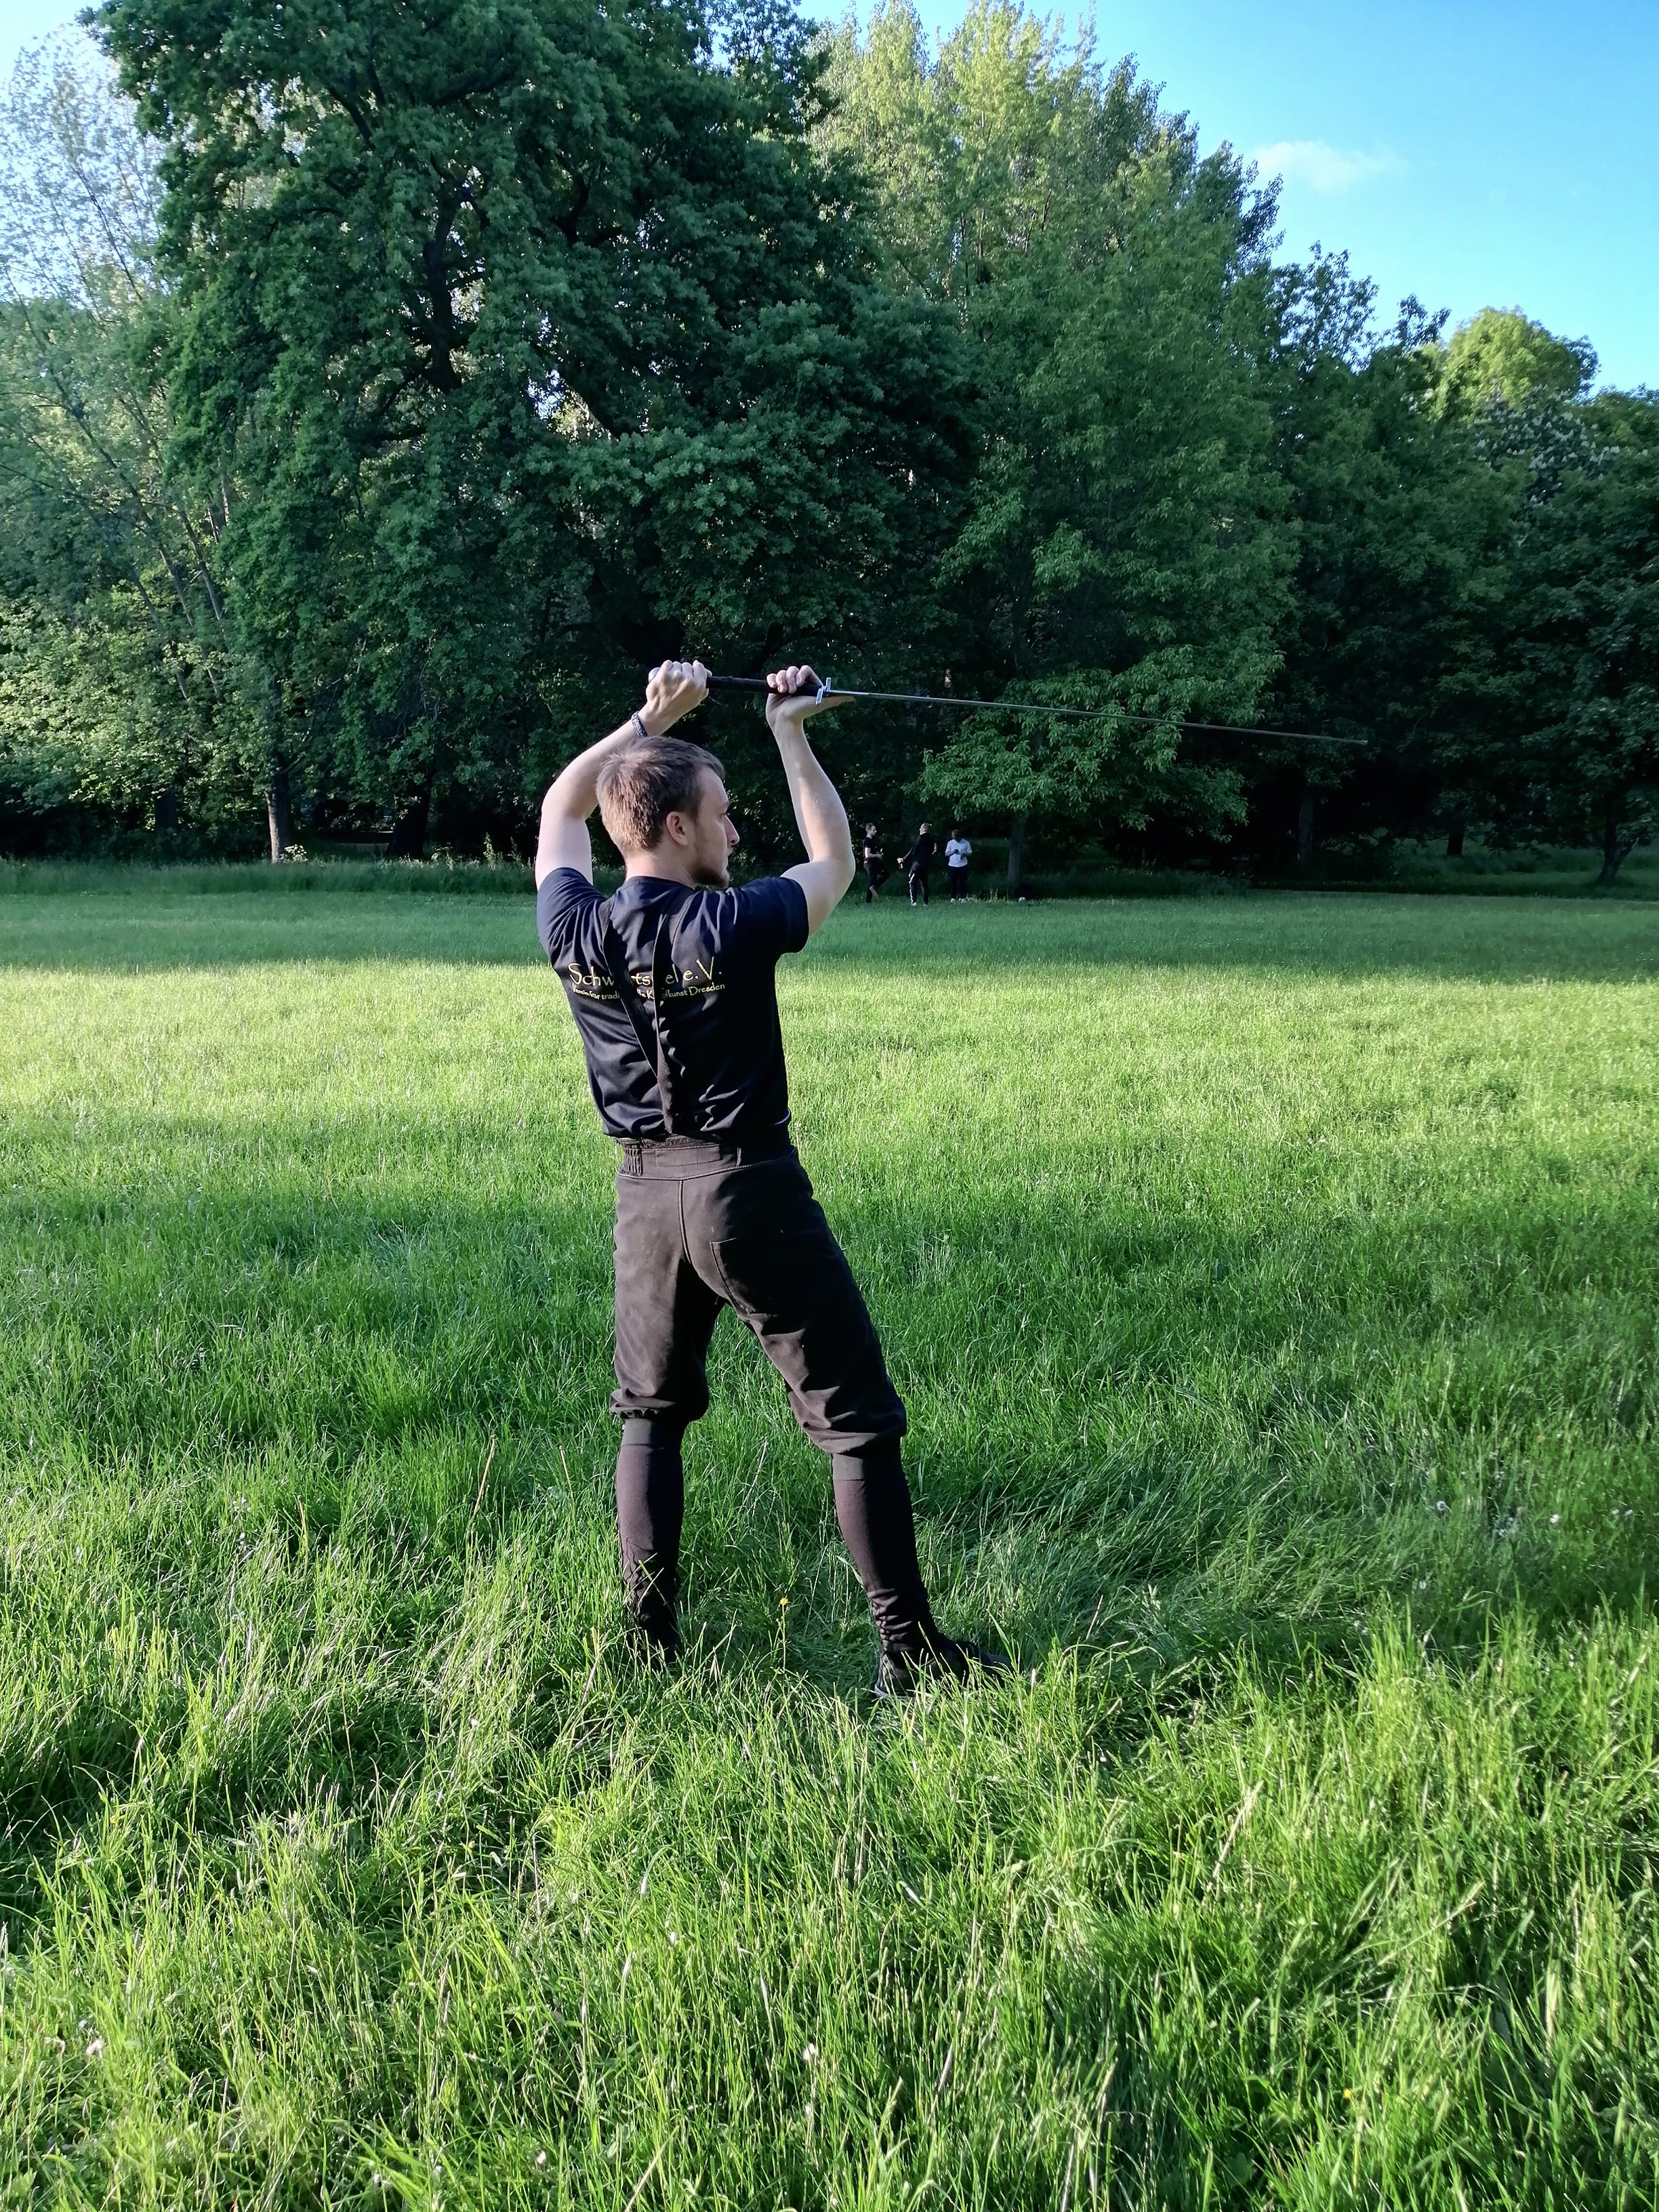
\includegraphics[width=\linewidth]{Ochs3.jpg}
  \caption{Ochs links}\label{fig:ochs3}
\endminipage
\end{figure}
\begin{figure}[ht!]
\minipage{0.32\textwidth}
  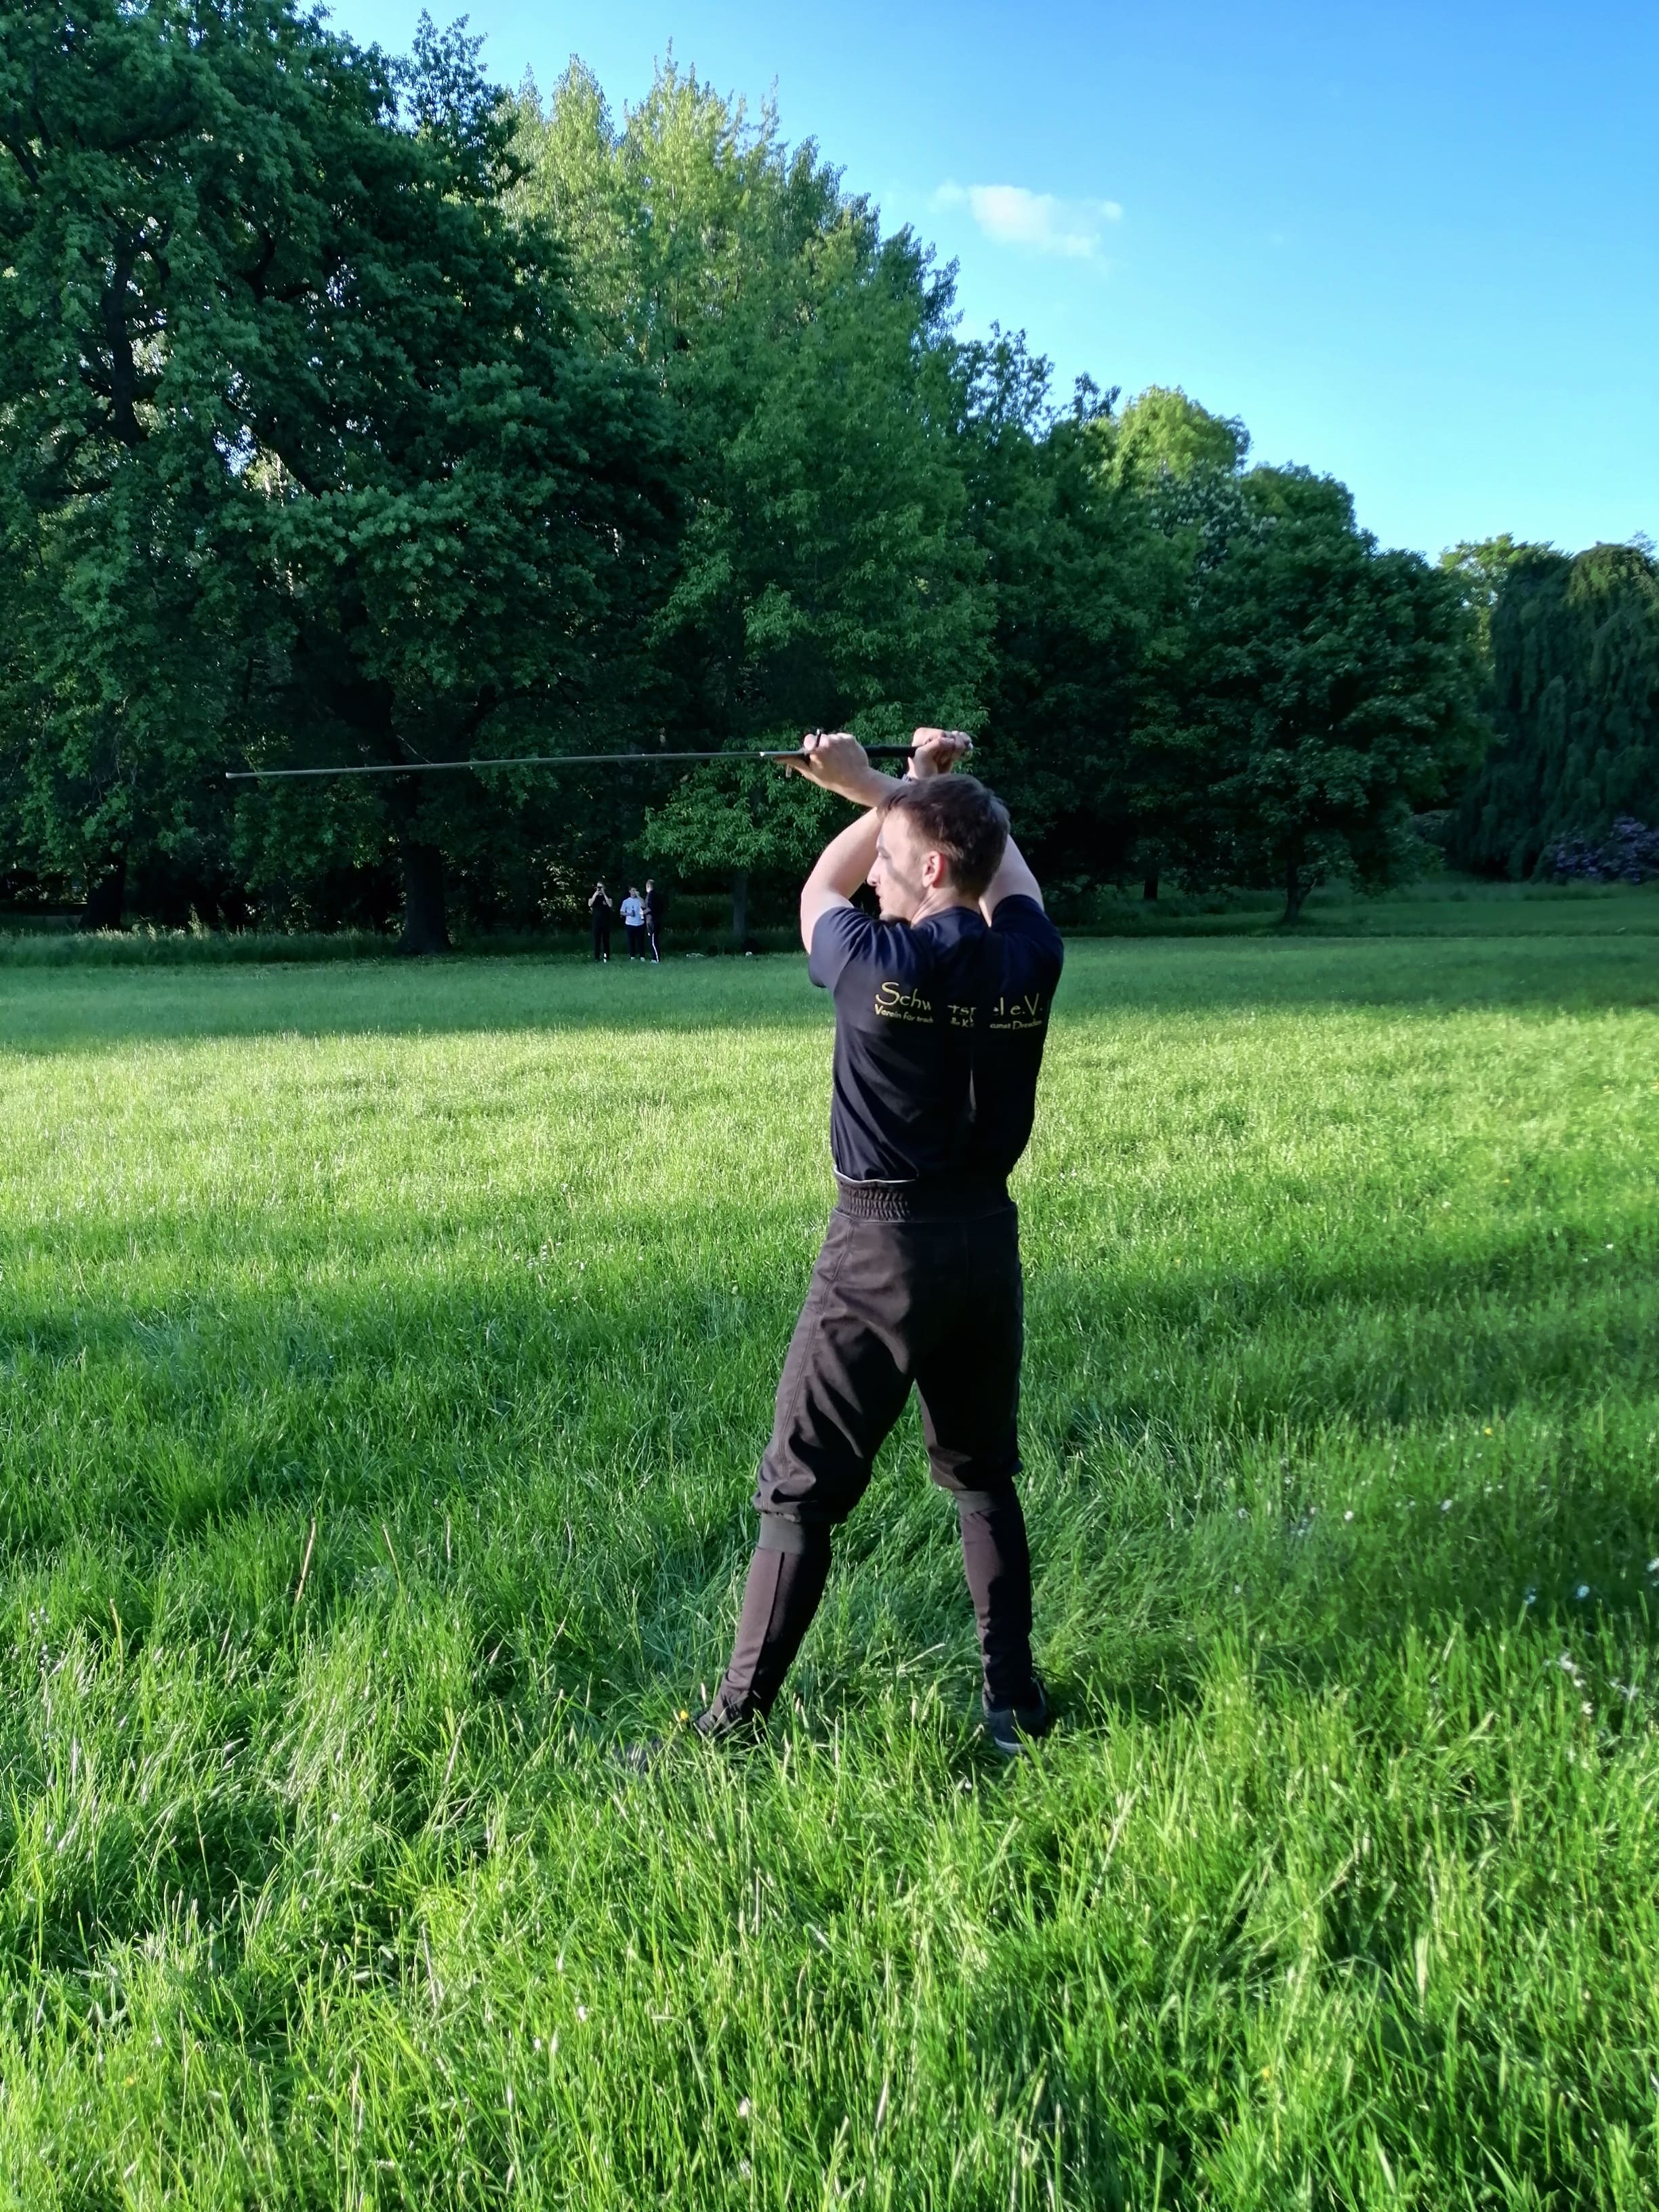
\includegraphics[width=\linewidth]{Ochs4.jpg}
  \caption{Ochs rechts}\label{fig:ochs4}
\endminipage\hfill
\minipage{0.32\textwidth}
  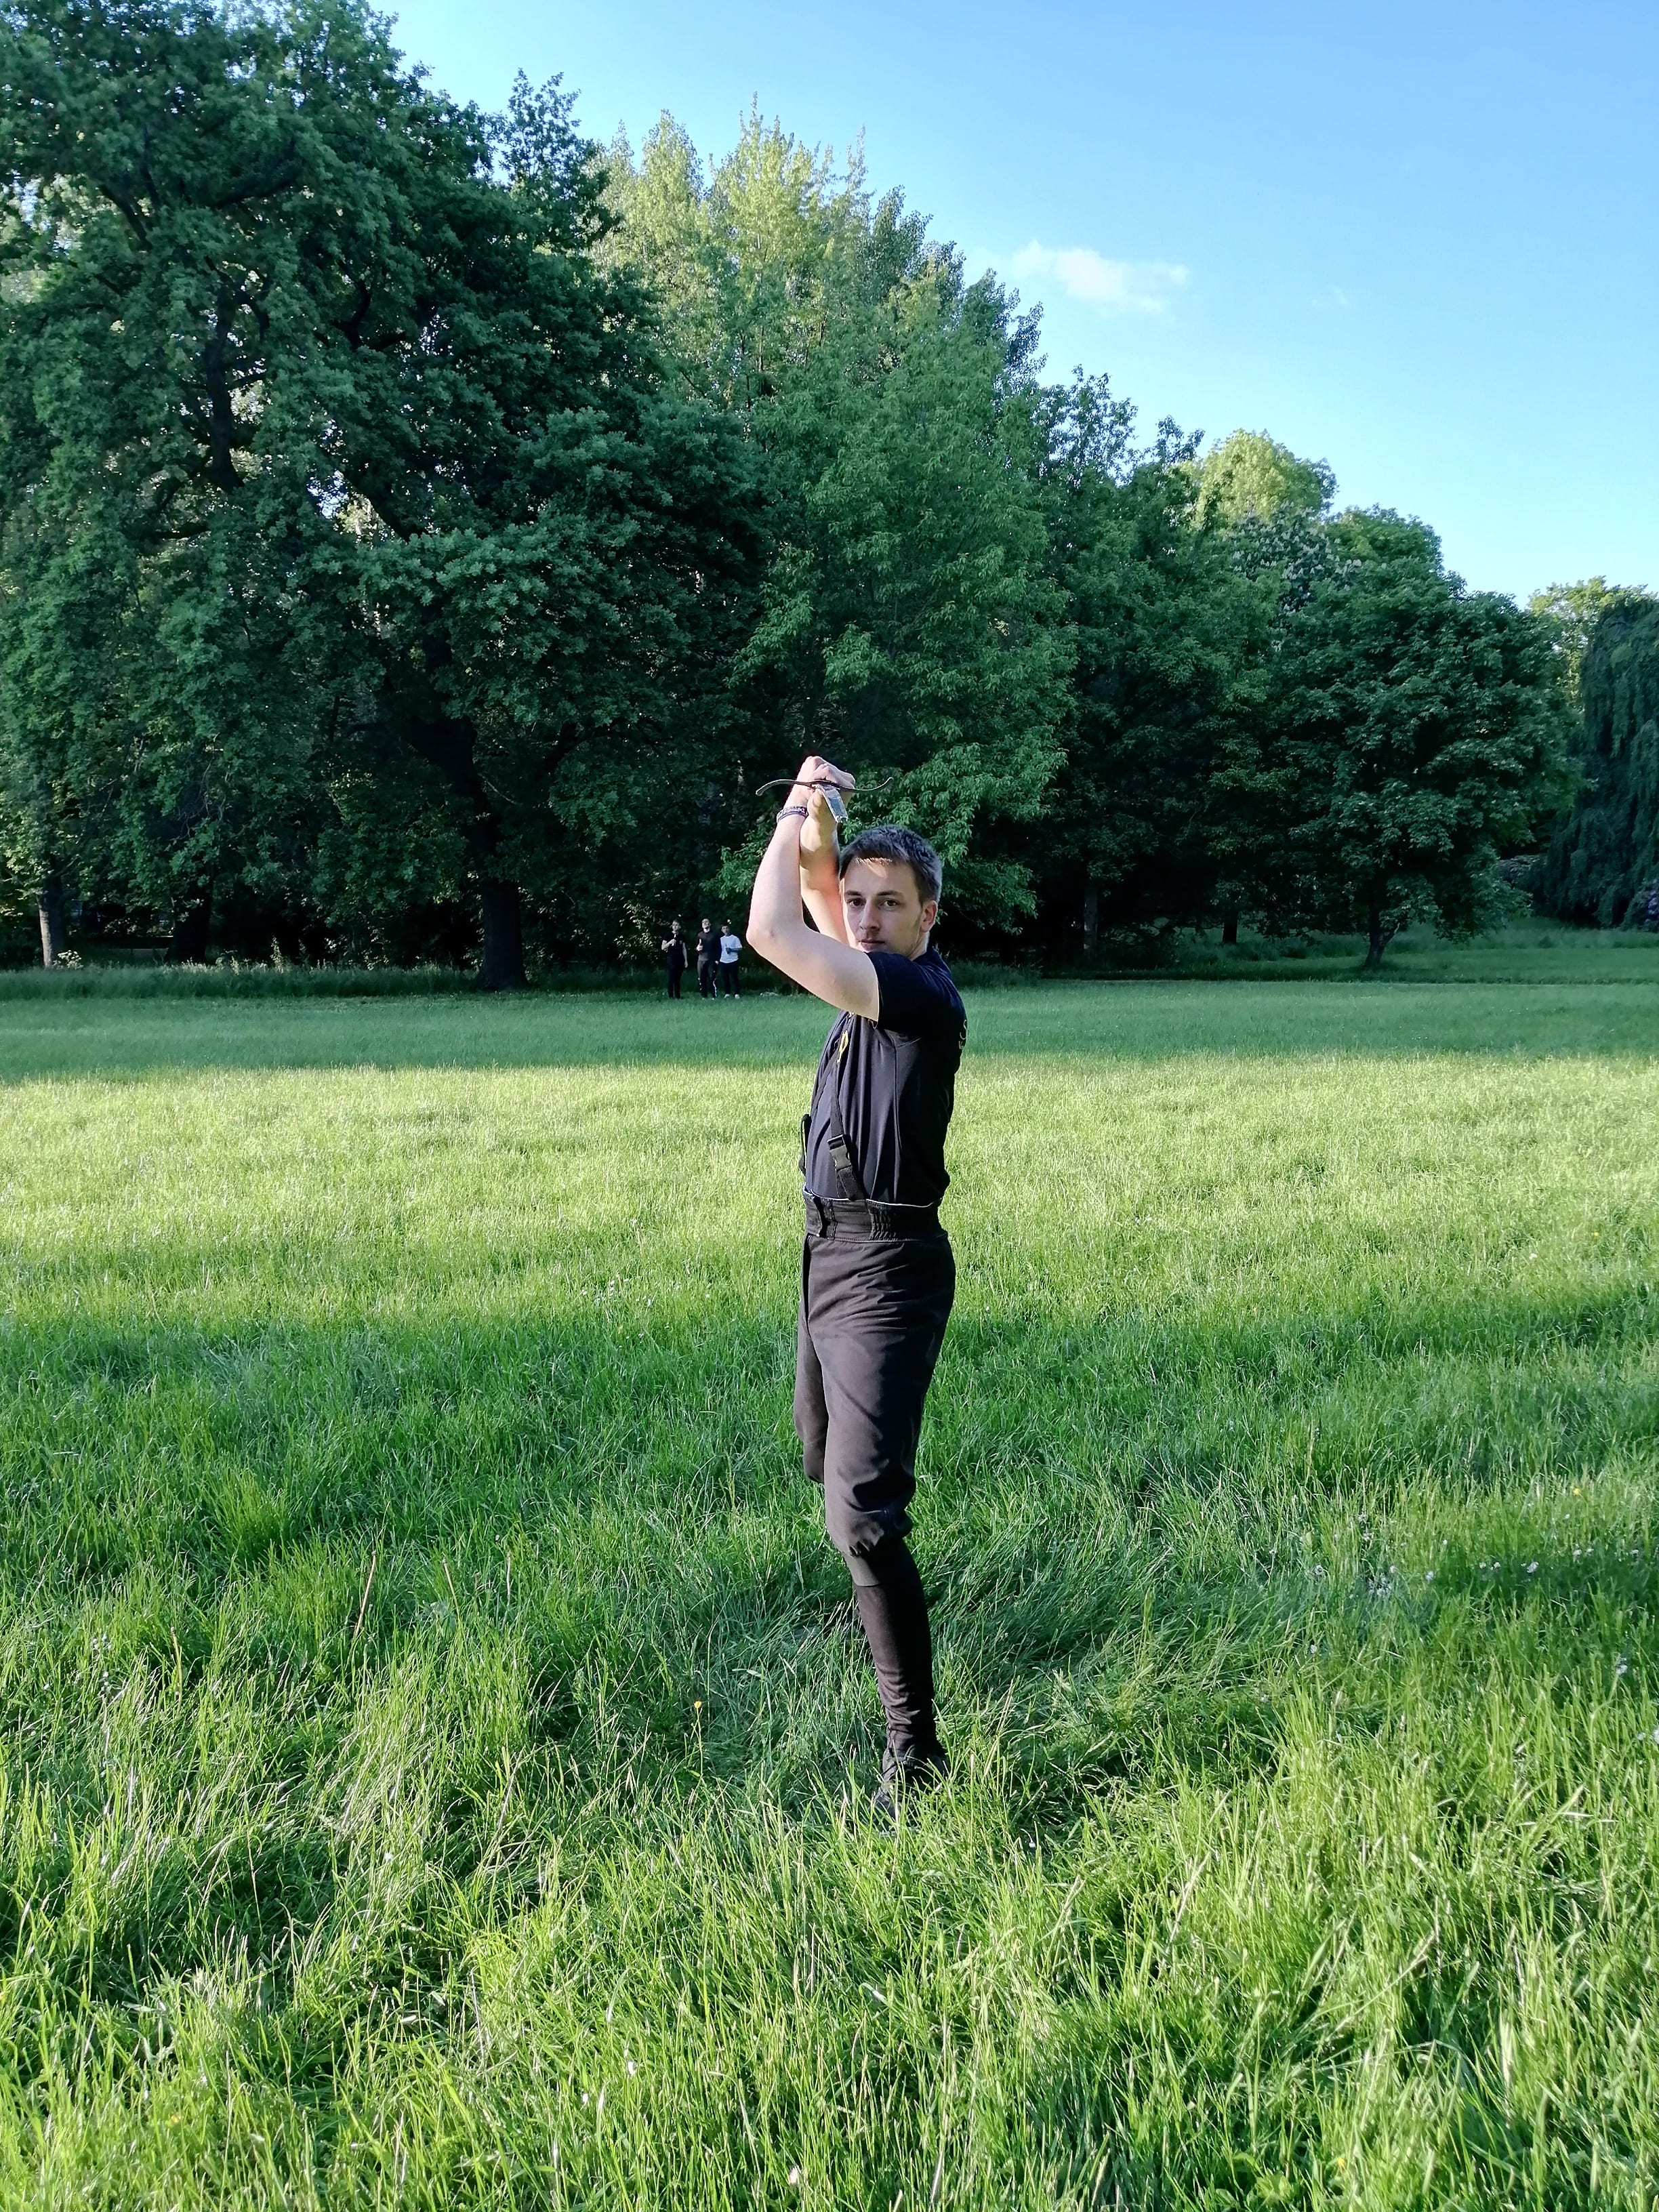
\includegraphics[width=\linewidth]{Ochs5.jpg}
  \caption{Ochs rechts}\label{fig:ochs5}
\endminipage\hfill
\minipage{0.32\textwidth}%
  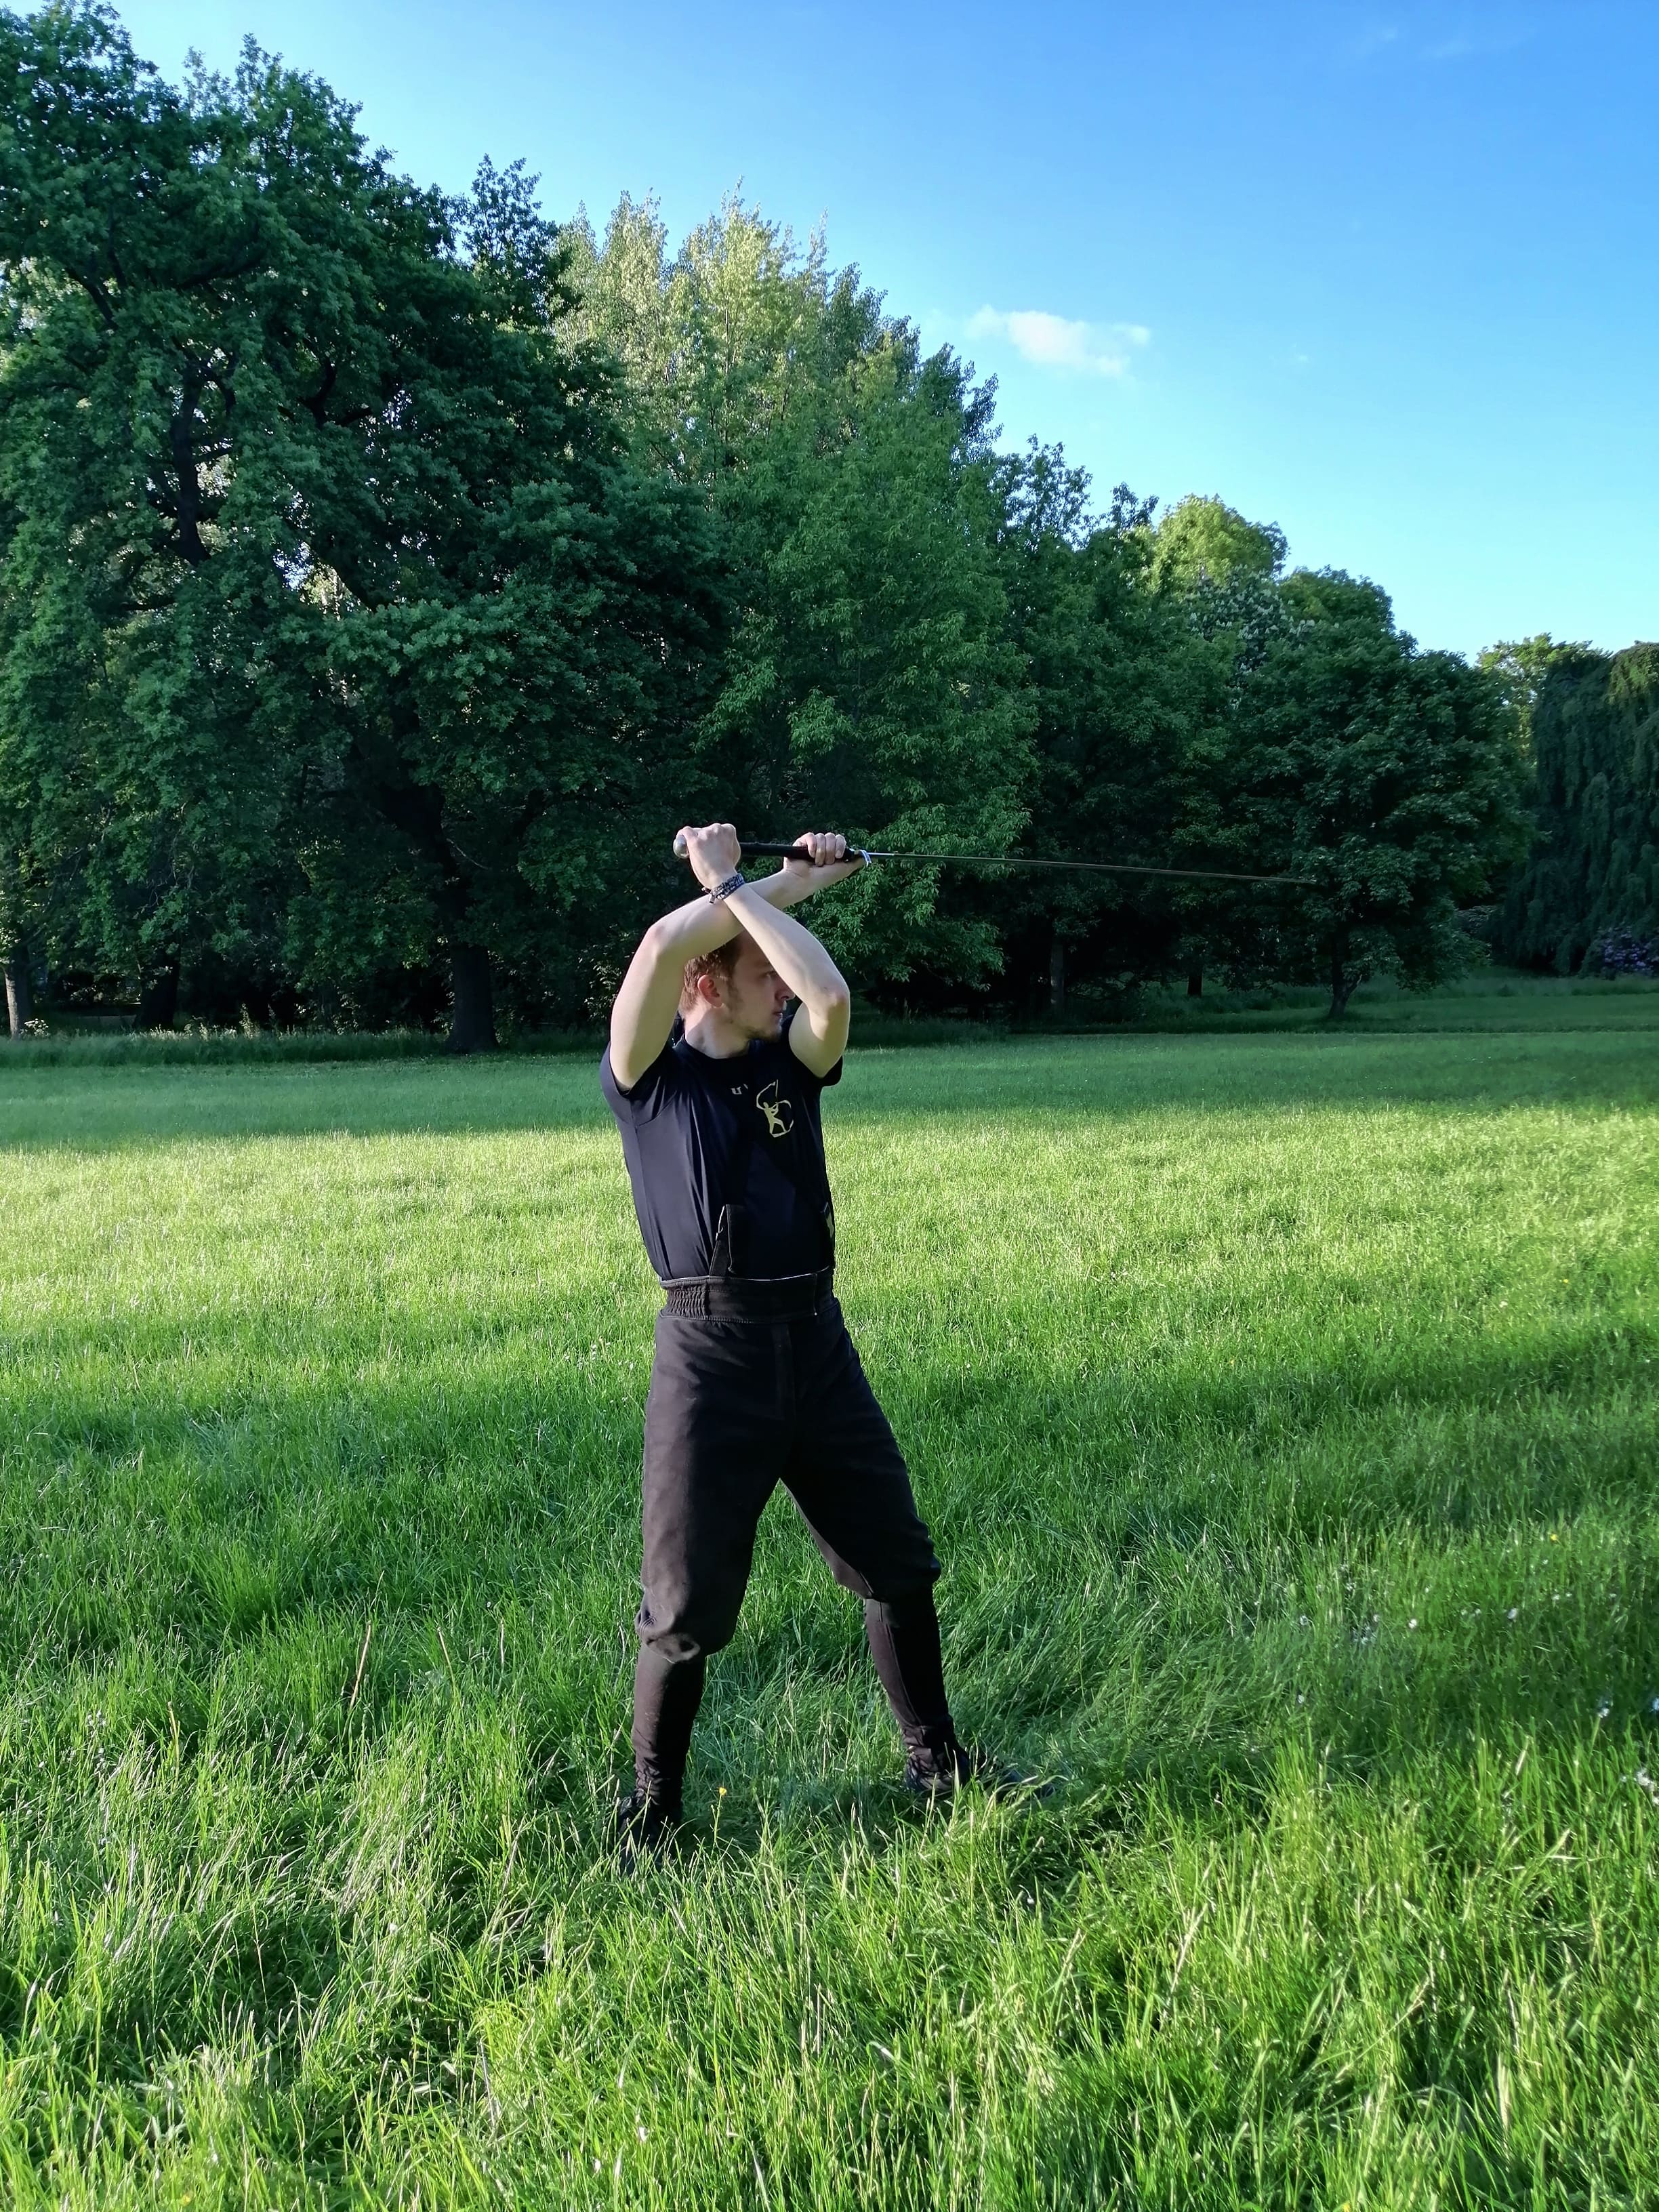
\includegraphics[width=\linewidth]{Ochs6.jpg}
  \caption{Ochs rechts}\label{fig:ochs6}
\endminipage
\end{figure}

Die Hut ''Ochs'' wird ebenfalls in links und rechts unterschieden. Die linke Seite unterscheidet sich von der Rechten in der Armhaltung: In der rechten Variante müssen (für Rechtshänder) die Arme gekreuzt werden, um das Schwert zu halten. Hierbei ist es wesentlich, dass die Handgelenke unter dem Schwert bleiben, um diese zu entlasten. Die Hände befinden sich etwas über Kopfhöhe. Der Ort ist zum Kopf oder Hals des Gegenübers gerichtet. Das Schwert wird im Daumengriff gehalten.

\newpage

\paragraph{Alber}

\begin{figure}[!ht]
\minipage{0.32\textwidth}
  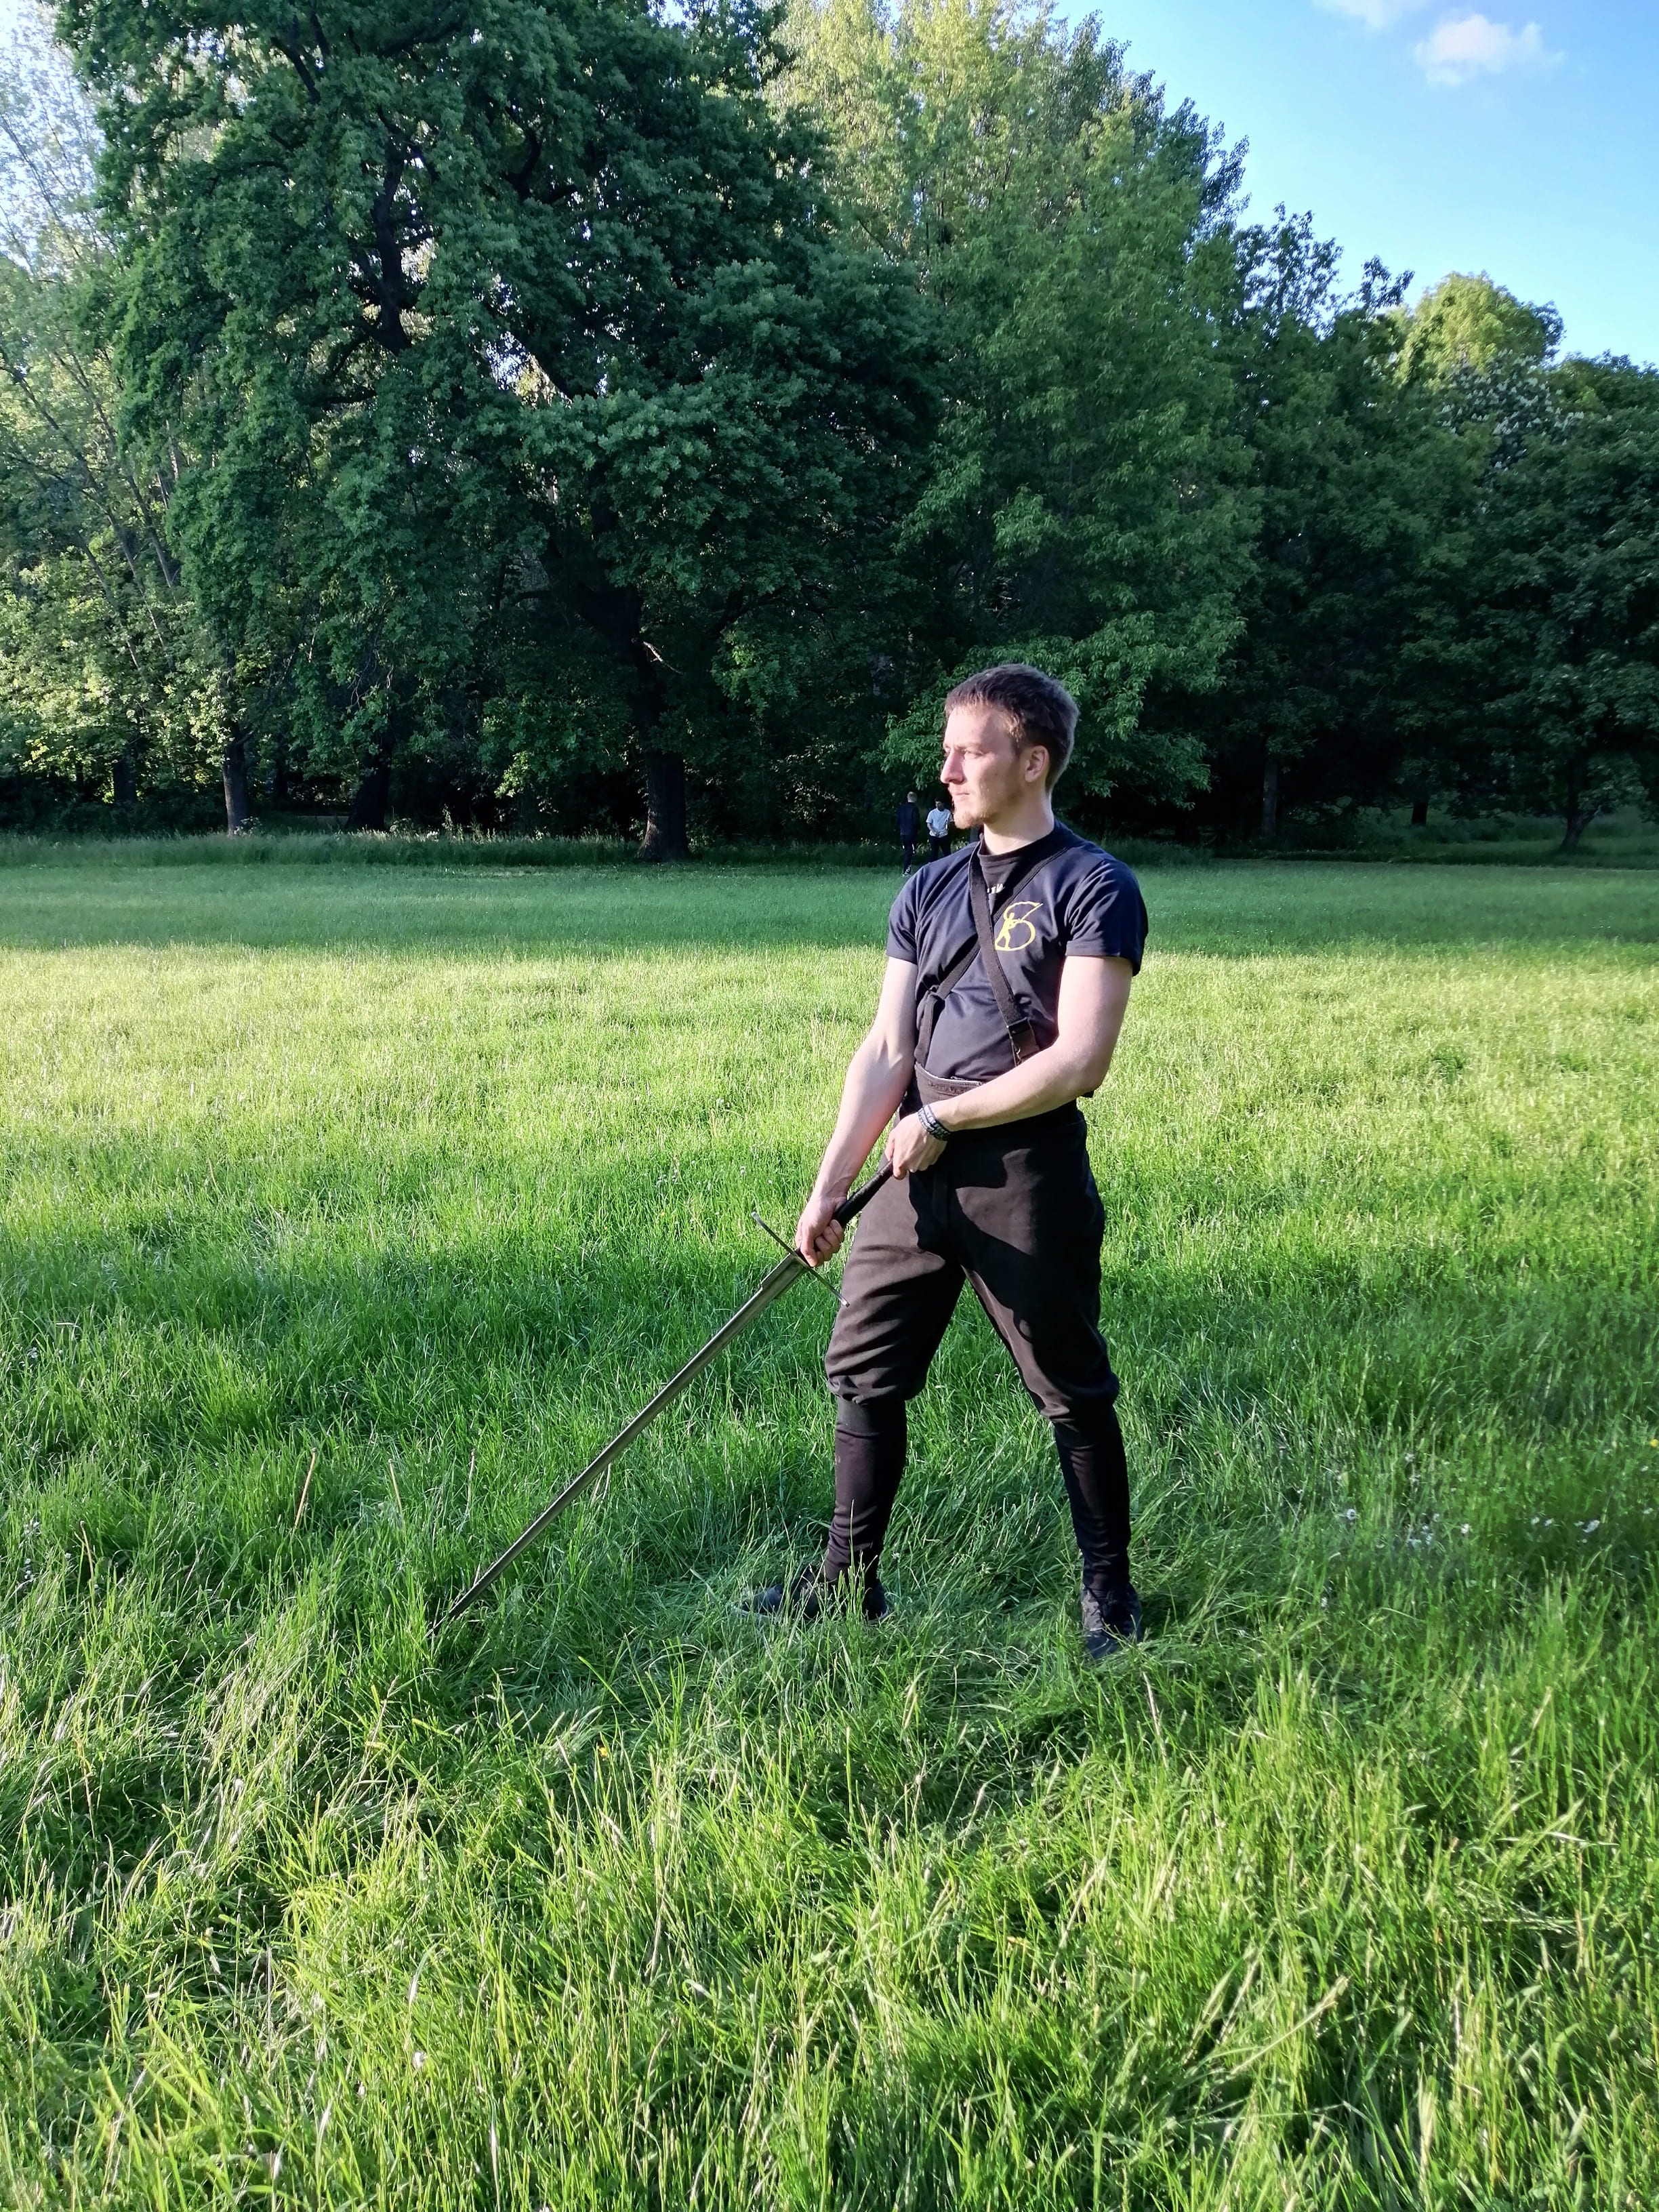
\includegraphics[width=\linewidth]{Alber1.jpg}
  \caption{links}\label{fig:alber1}
\endminipage\hfill
\minipage{0.32\textwidth}
  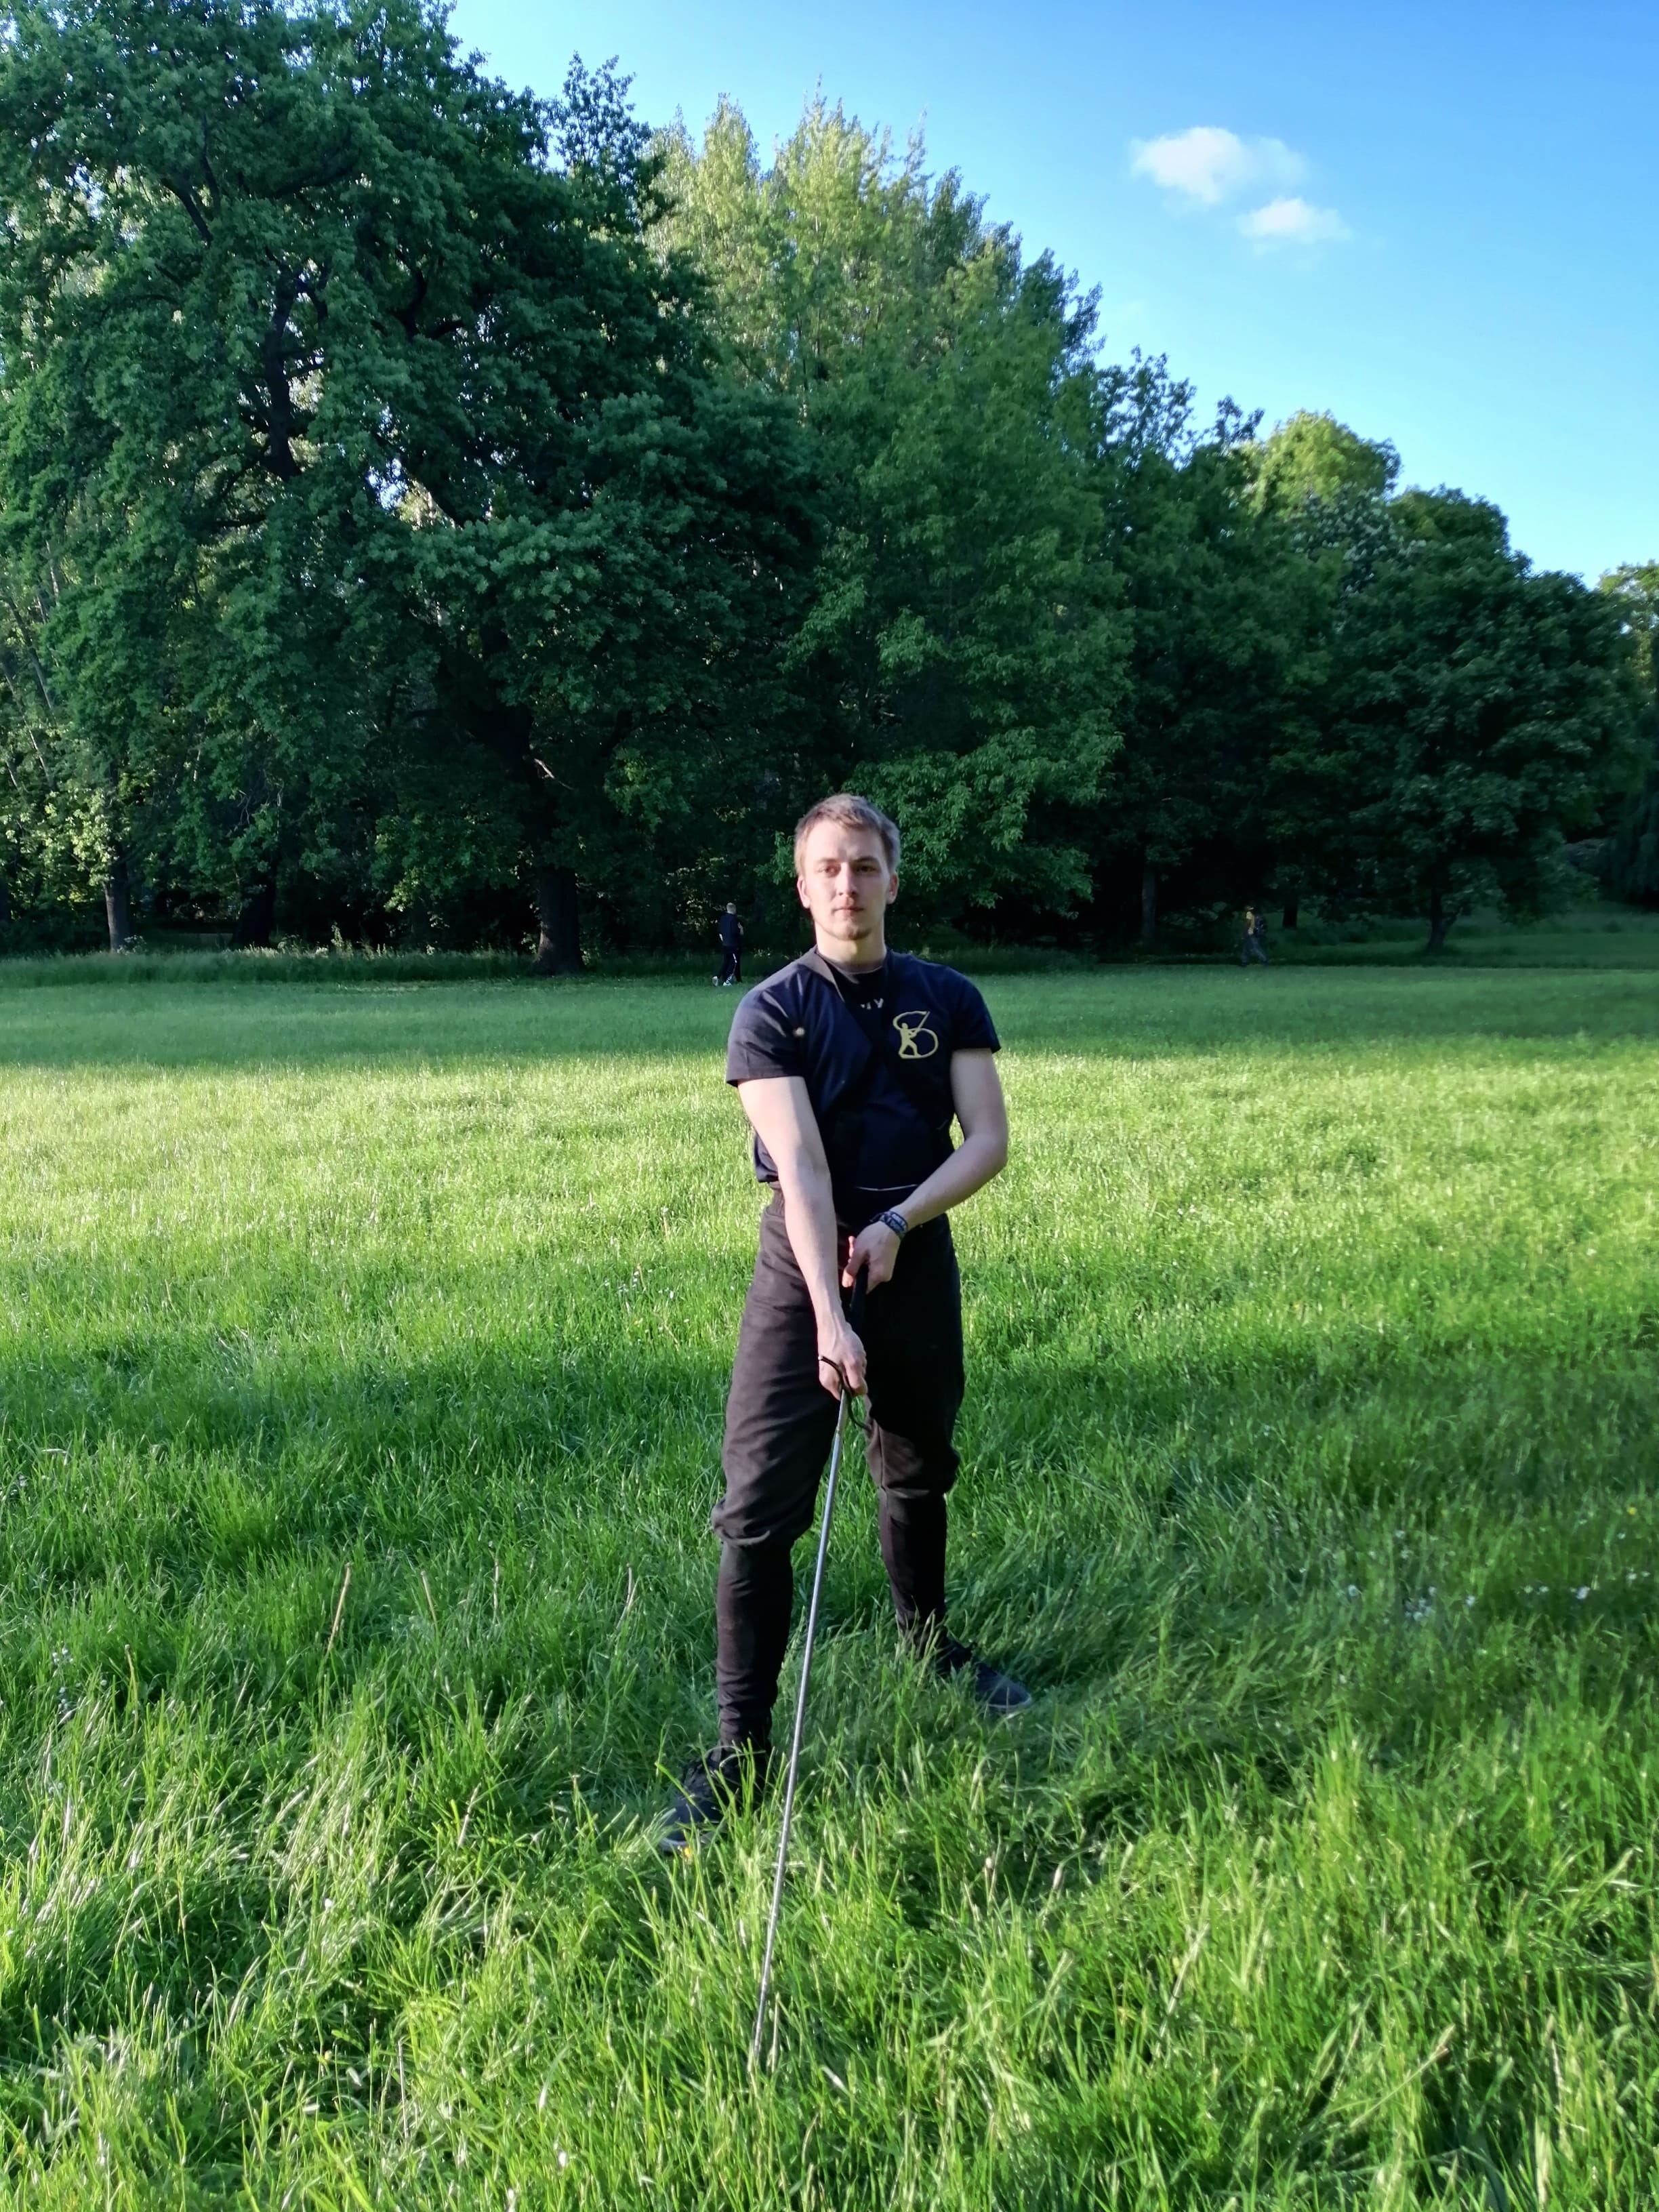
\includegraphics[width=\linewidth]{Alber2.jpg}
  \caption{frontal}\label{fig:alber2}
\endminipage\hfill
\minipage{0.32\textwidth}%
  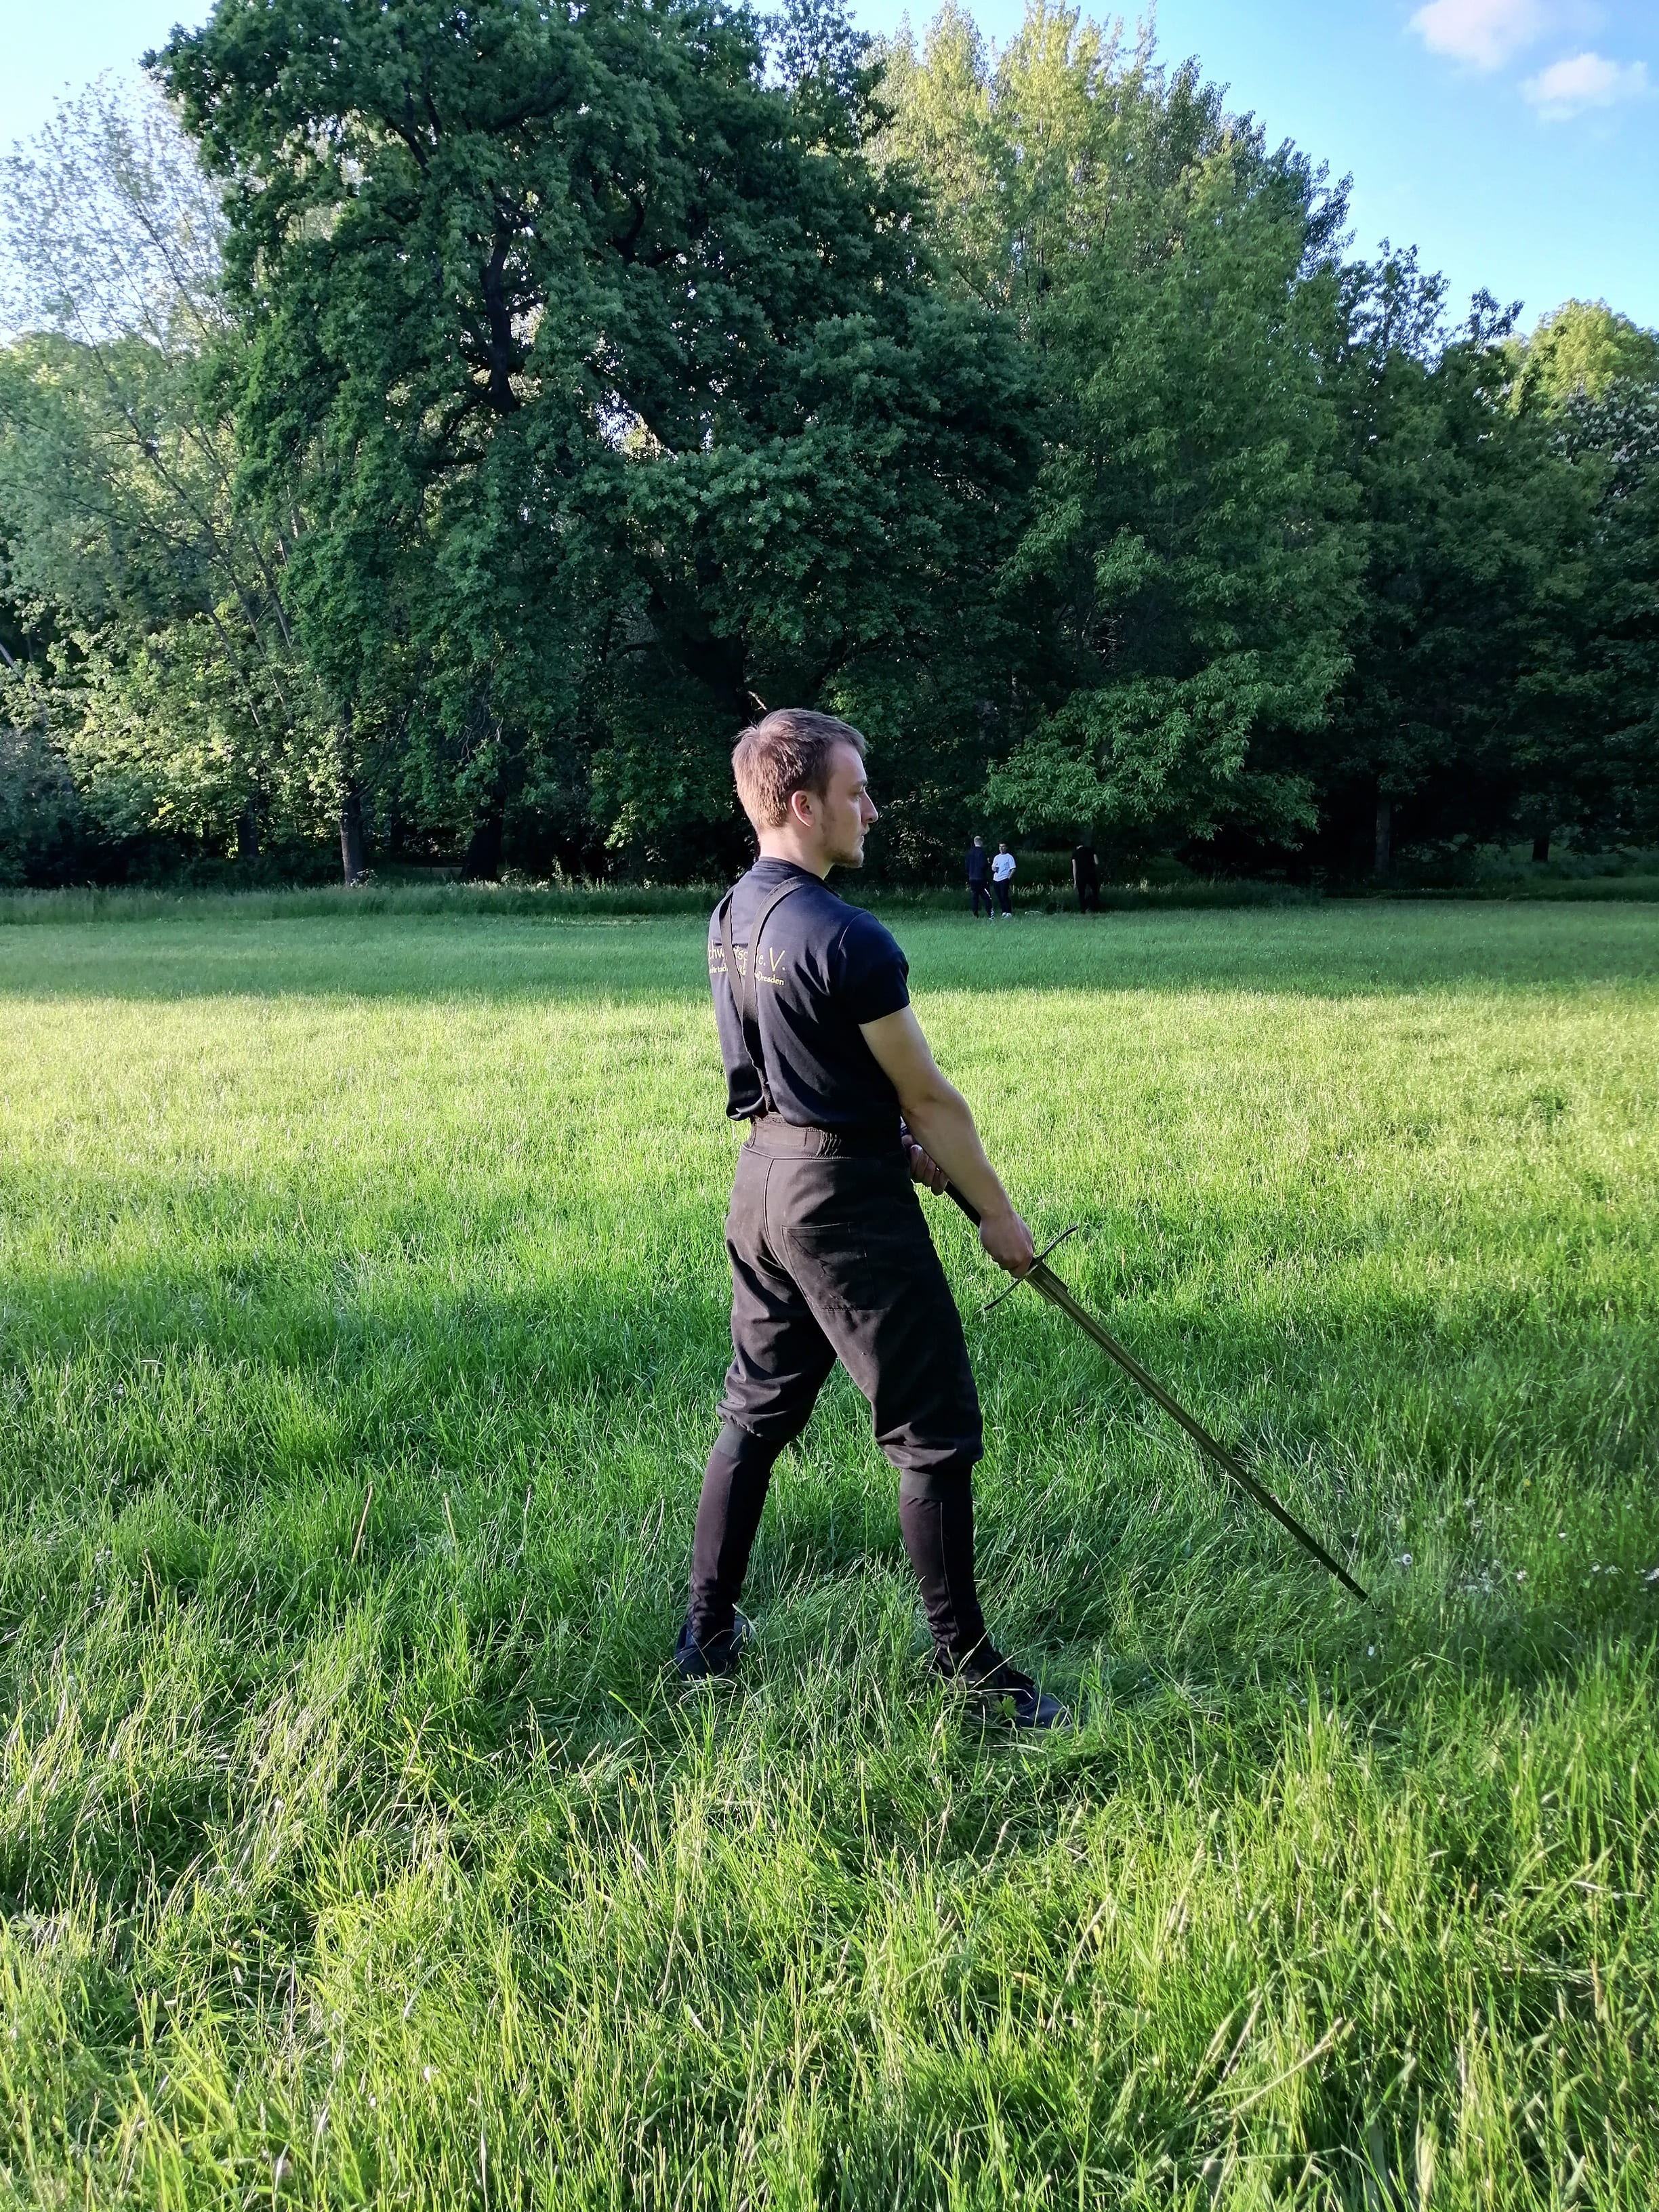
\includegraphics[width=\linewidth]{Alber3.jpg}
  \caption{rechts}\label{fig:alber3}
\endminipage
\end{figure}

Die Hut ''Alber'' kennt nur die neutrale Position. Daher kann die Fußstellung frei gewählt werden. Es empfiehlt sich, vorausschauend eine Fußstellung und Griffweise so zu wählen, dass sie die geplante Aktion unterstützen.
\\
\FloatBarrier
\hrule

\begin{figure}[!ht]
\minipage{0.5\textwidth}
  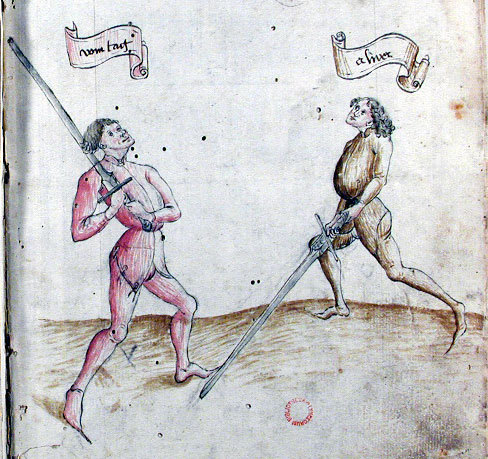
\includegraphics[width=\linewidth]{Haupthuten1.jpg}
  \caption{Vom Tag und Alber}\label{fig:haupthuten1}
\endminipage\hfill
\minipage{0.4\textwidth}
  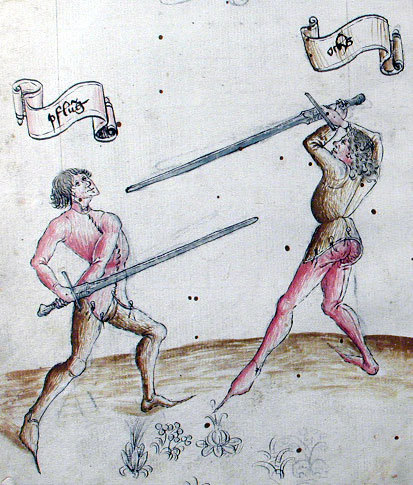
\includegraphics[width=\linewidth]{Haupthuten2.jpg}
  \caption{Ochs und Pflug}\label{fig:haupthuten2}
\endminipage\hfill
\end{figure}

\FloatBarrier

Die Darstellung der Huten im Codex 44 A 8, 1452

\newpage

\subsubsection{Blößen}

Das finale Ziel aller Aktionen im Fechten sollte es sein, das Gegenüber zu treffen, ohne dabei selbst getroffen zu werden. Dazu entstand sowohl in der italienischen, als auch in der deutschen Fechtart das Prinzip der ''Blößen''. Die Blößen beschreiben potentielle Ziele, welche nicht durch das Schwert geschützt werden. Das Wissen über die eigenen Blößen, die Blößen des Gegenübers und wie diese möglichst effizient zu schützen, bzw. zu erreichen sind, ist deshalb essentiell für alle Entscheidungen in einem Gefecht.
\\
\\
In einem Dresdner Manuskript\footnote{\hspace*{0.5ex}Dresden, SLUB, Mscr.Dresd.C.487, fol. 22v-23r, eigene Transkription und Übersetzung.} steht dazu:
\\
\\
(22v) Vier Blößen wisse zu nehmen, so schlägst Du gewisse, alle Vier. Ohne Zweifel, (egal) wie er sich gebärdet.
\\
\\
(22v-23r) Hier sollst Du Dir die vier Blößen an dem Mann merken, dass Du diesen immer zufechten sollst. Die erste Blöße ist die rechte Seite, die Andere ist die linke Seite, oberhalb des Gürtels des Mannes.
\\
\\
Die anderen Zwei sind die rechte und die linke Seite unterhalb des Gürtels. Diese Blößen nehmen eben wahr, in dem Zufechten. Mit welcher Blöße er sich gegen Dich entblößt. Diese greife künstlich ohne Gefahr an. Mit dem Einschießen des Langen Ortes, mit Nachreisen und sonst mit allen Gefechten. Und achte nicht darauf, wie er sich mit seinen Gefechten gegen Dich verhält.So fechtest Du sicher und schlägst Schläge daraus, die sehr trefflich sind und lässt ihn damit nicht zu seinen Stücken kommen.''

\begin{figure}
    \centering
    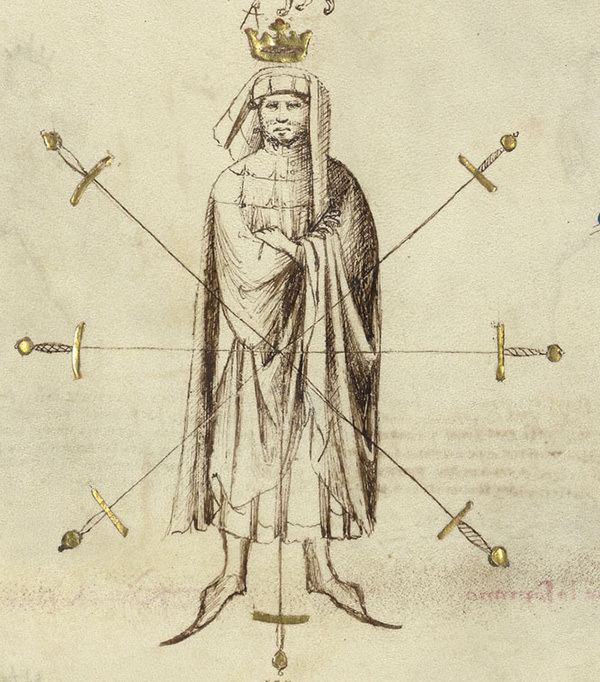
\includegraphics[scale=.27]{fiore-dei-liberi.jpeg}
    \caption{Darstellung der Blößen, ''Fior di Battaglia'' (MS Ludwig XV 13, 1404)}
    \label{fig:Blößen}
\end{figure}

% Quelle http://fechtfabrik.de/fiore-dei-liberi/
% unter  CopyLeft Lizenz

\FloatBarrier

\newpage

\subsubsection{Mensur}

Der Abstand zum:zur Gegner:in wird allgemein als ''Mensur'' bezeichnet. Bestimmte Techniken erfordern eine bestimmte Mensur. Die Fähigkeit, Mensur einzuschätzen, sowie das Wissen darüber, welche Technik in welcher Situation optimal ist, sind Schlüssel zum erfolgreichen Fechten. Sie erlauben es, erfolgreich die Initiative zu ergreifen und machen das Gefecht berechenbarer.

\paragraph{Zufechtmensur}

\FloatBarrier

\begin{figure}[!ht]
    \centering
    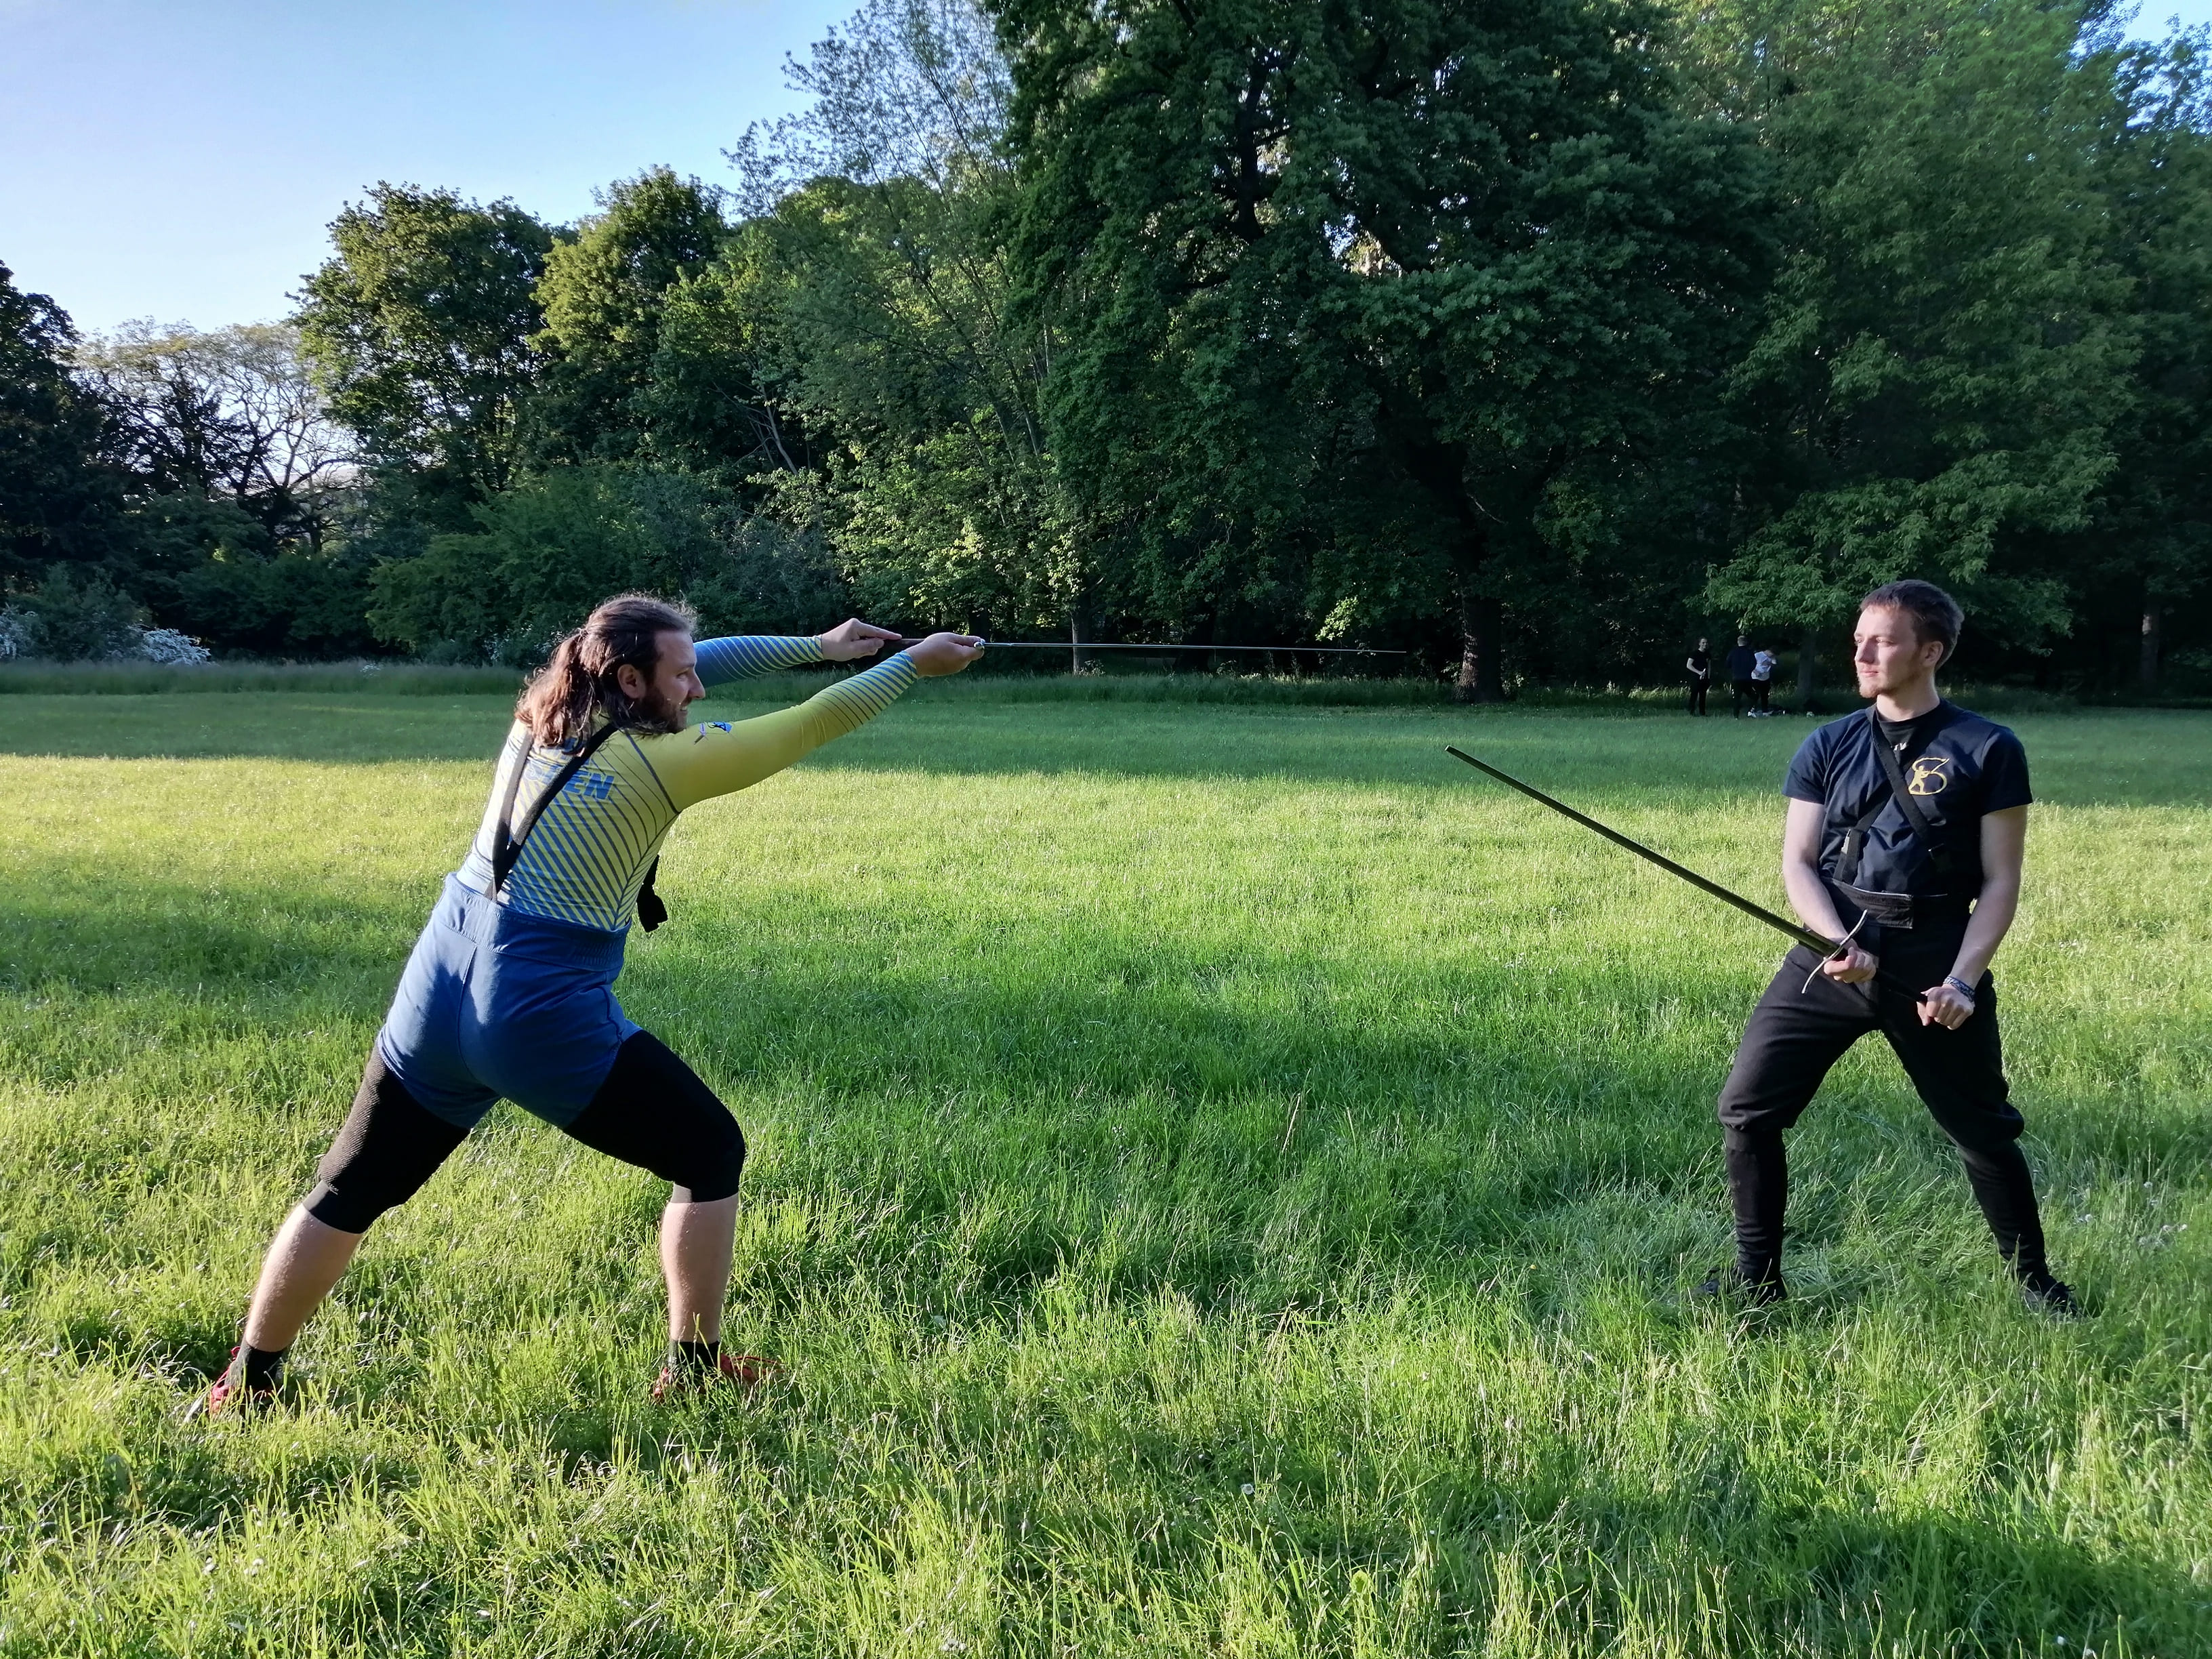
\includegraphics[scale=.05]{Weite2.jpg}
    \caption{Die Zufechtmensur}
    \label{fig:Zufechtmensur}
\end{figure}

Der:die Gegner:in kann mit der Klinge und nur einem Schritt erreicht werden.
\\
\FloatBarrier
\hrule
%\newpage

\paragraph{Kriegsmensur}

\FloatBarrier

\begin{figure}[!ht]
\minipage{0.45\textwidth}
  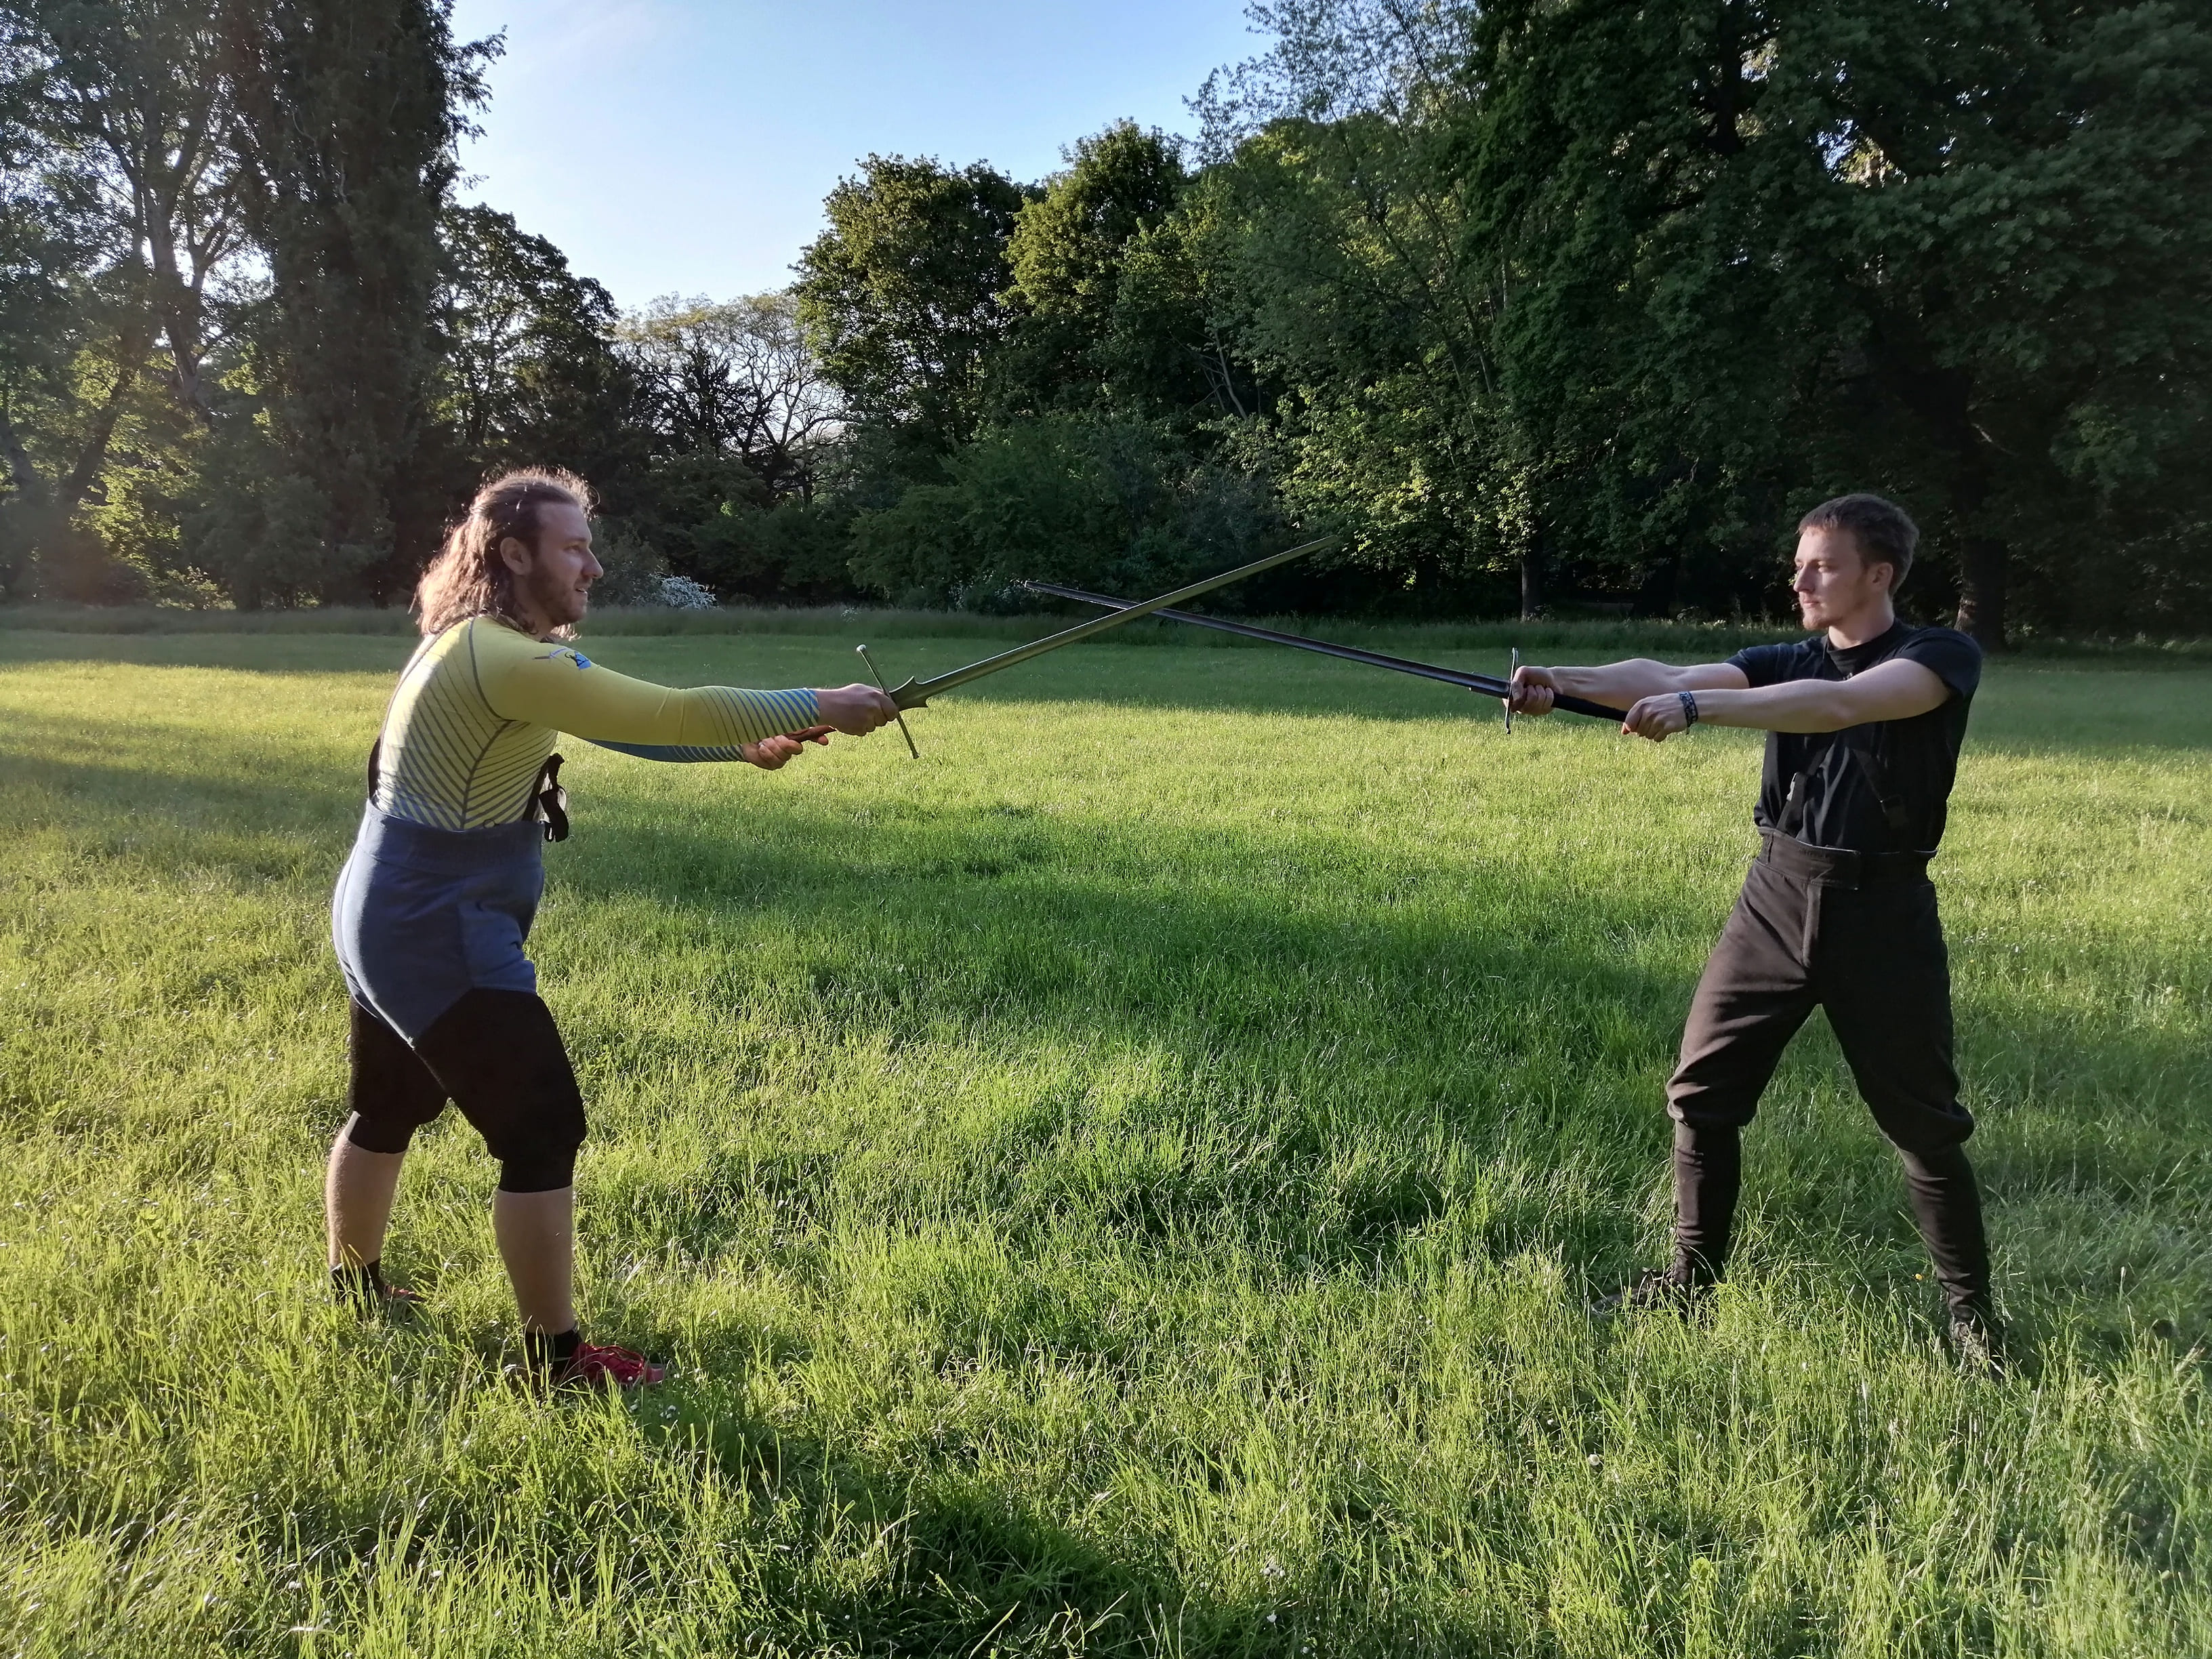
\includegraphics[width=\linewidth]{Langort.jpg}
  \caption{Eintritt in die Kriegsmensur}\label{fig:krieg1}
\endminipage\hfill
\minipage{0.45\textwidth}
  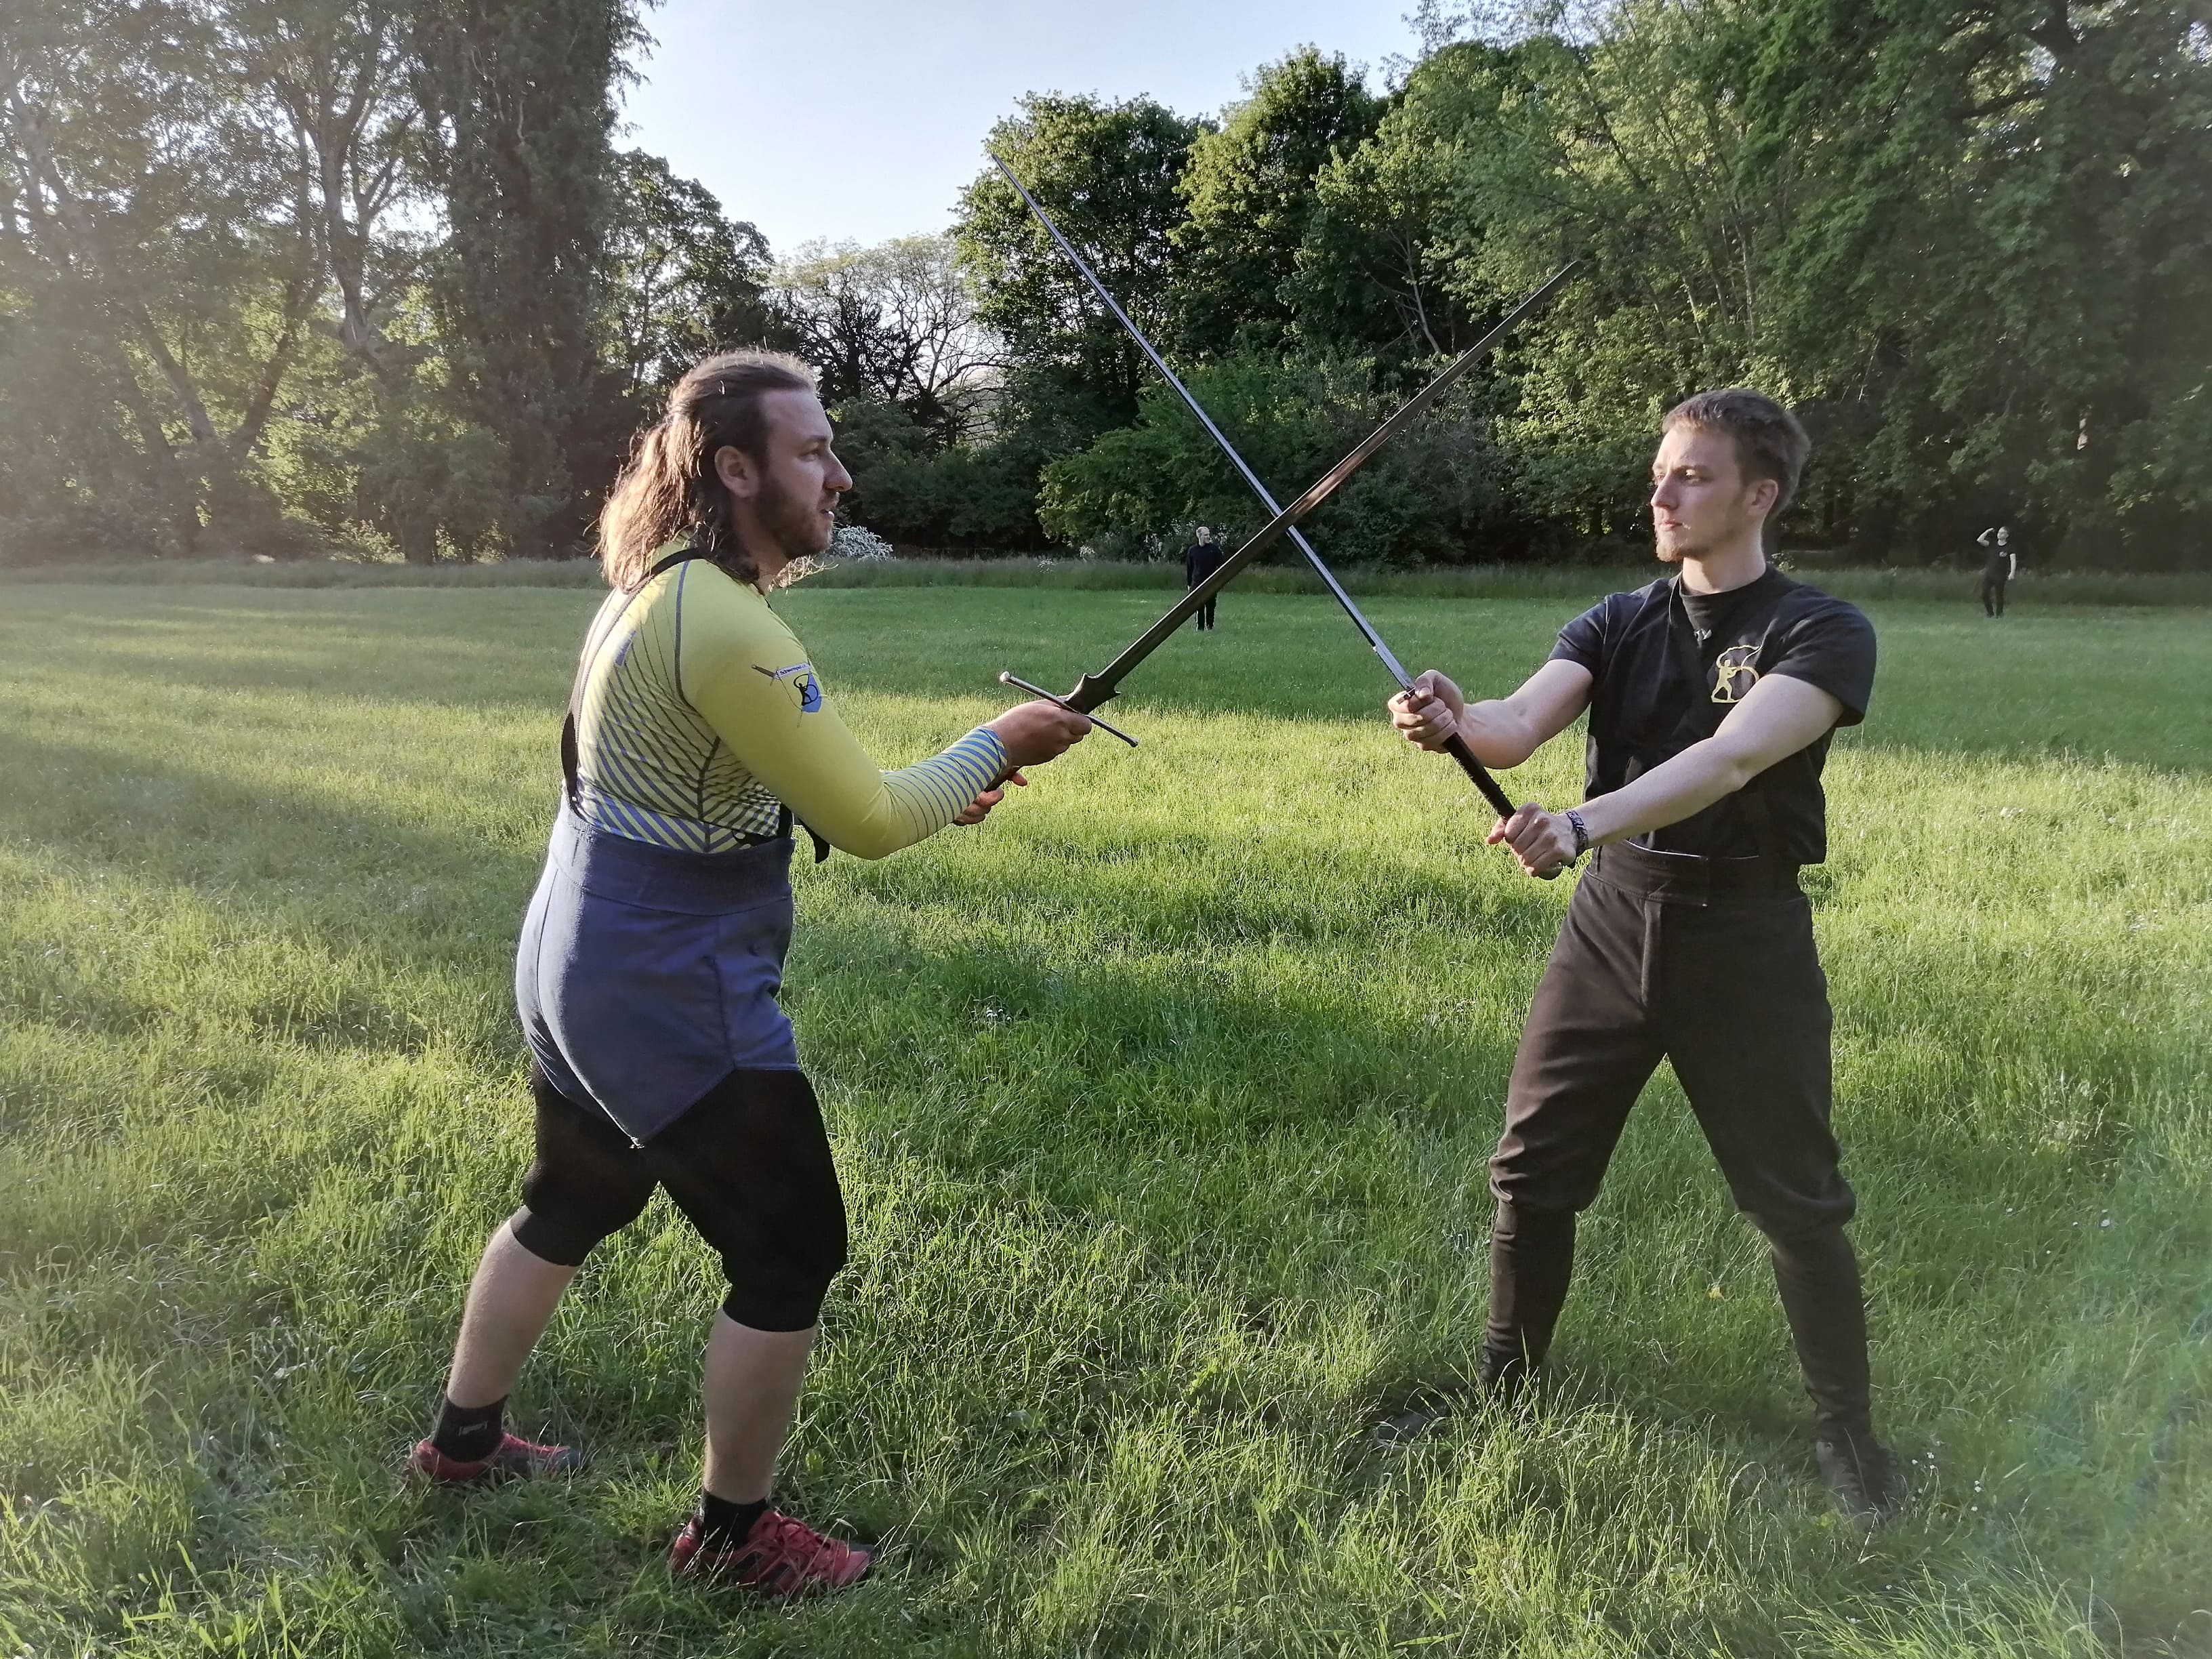
\includegraphics[width=\linewidth]{Schnitt1.jpg}
  \caption{Austritt aus der Kriegsmensur}\label{fig:krieg2}
\endminipage\hfill

\end{figure}

Das Gegenüber ist ohne Schritt erreichbar. Hier geschieht die Bindungsarbeit.

\FloatBarrier

\newpage

\paragraph{Ringmensur I: Das Armringen}

\begin{figure}[!ht]
    \centering
    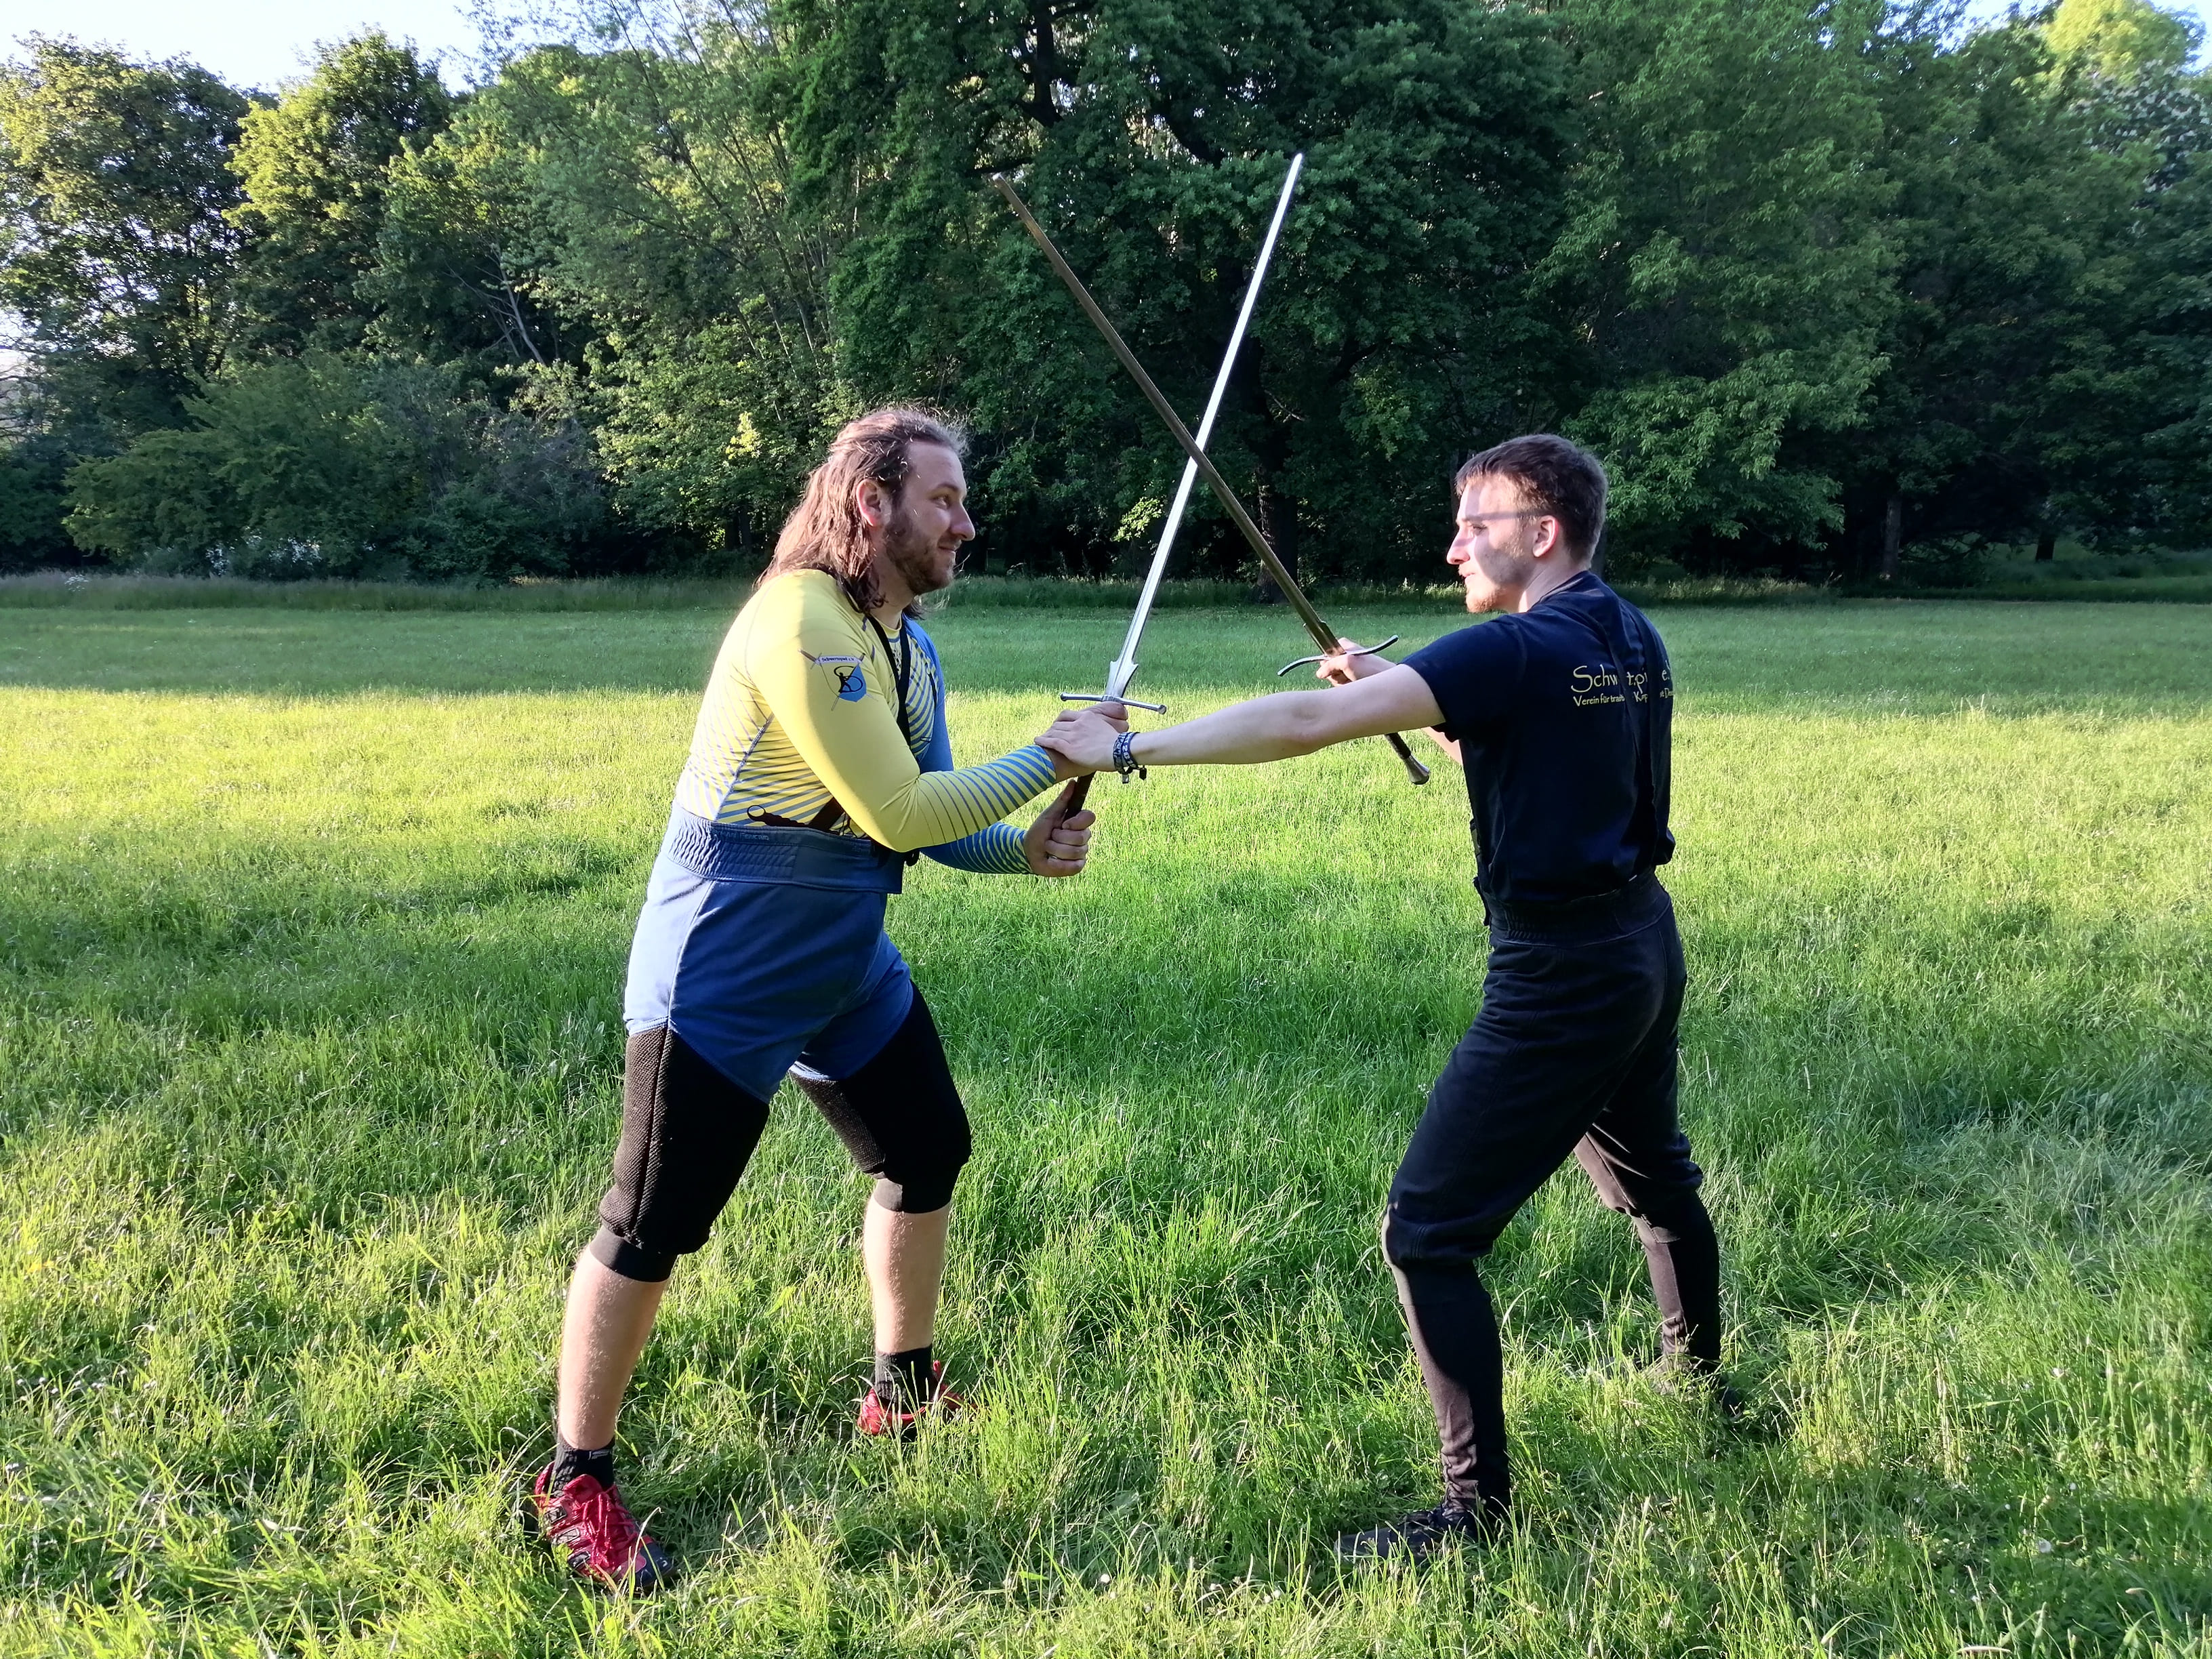
\includegraphics[scale=.05]{Eng1.jpg}
    \caption{Das Armringen}
    \label{fig:Armringen}
\end{figure}

Man erreicht mit der eignen Hand die Arme des Gegenübers. Armringen und Schwertnehmen sind möglich, weite Häue verlieren an Effekt.
\\
\hrule

\paragraph{Ringmensur II: Das Leibringen}

\begin{figure}[!ht]
    \centering
    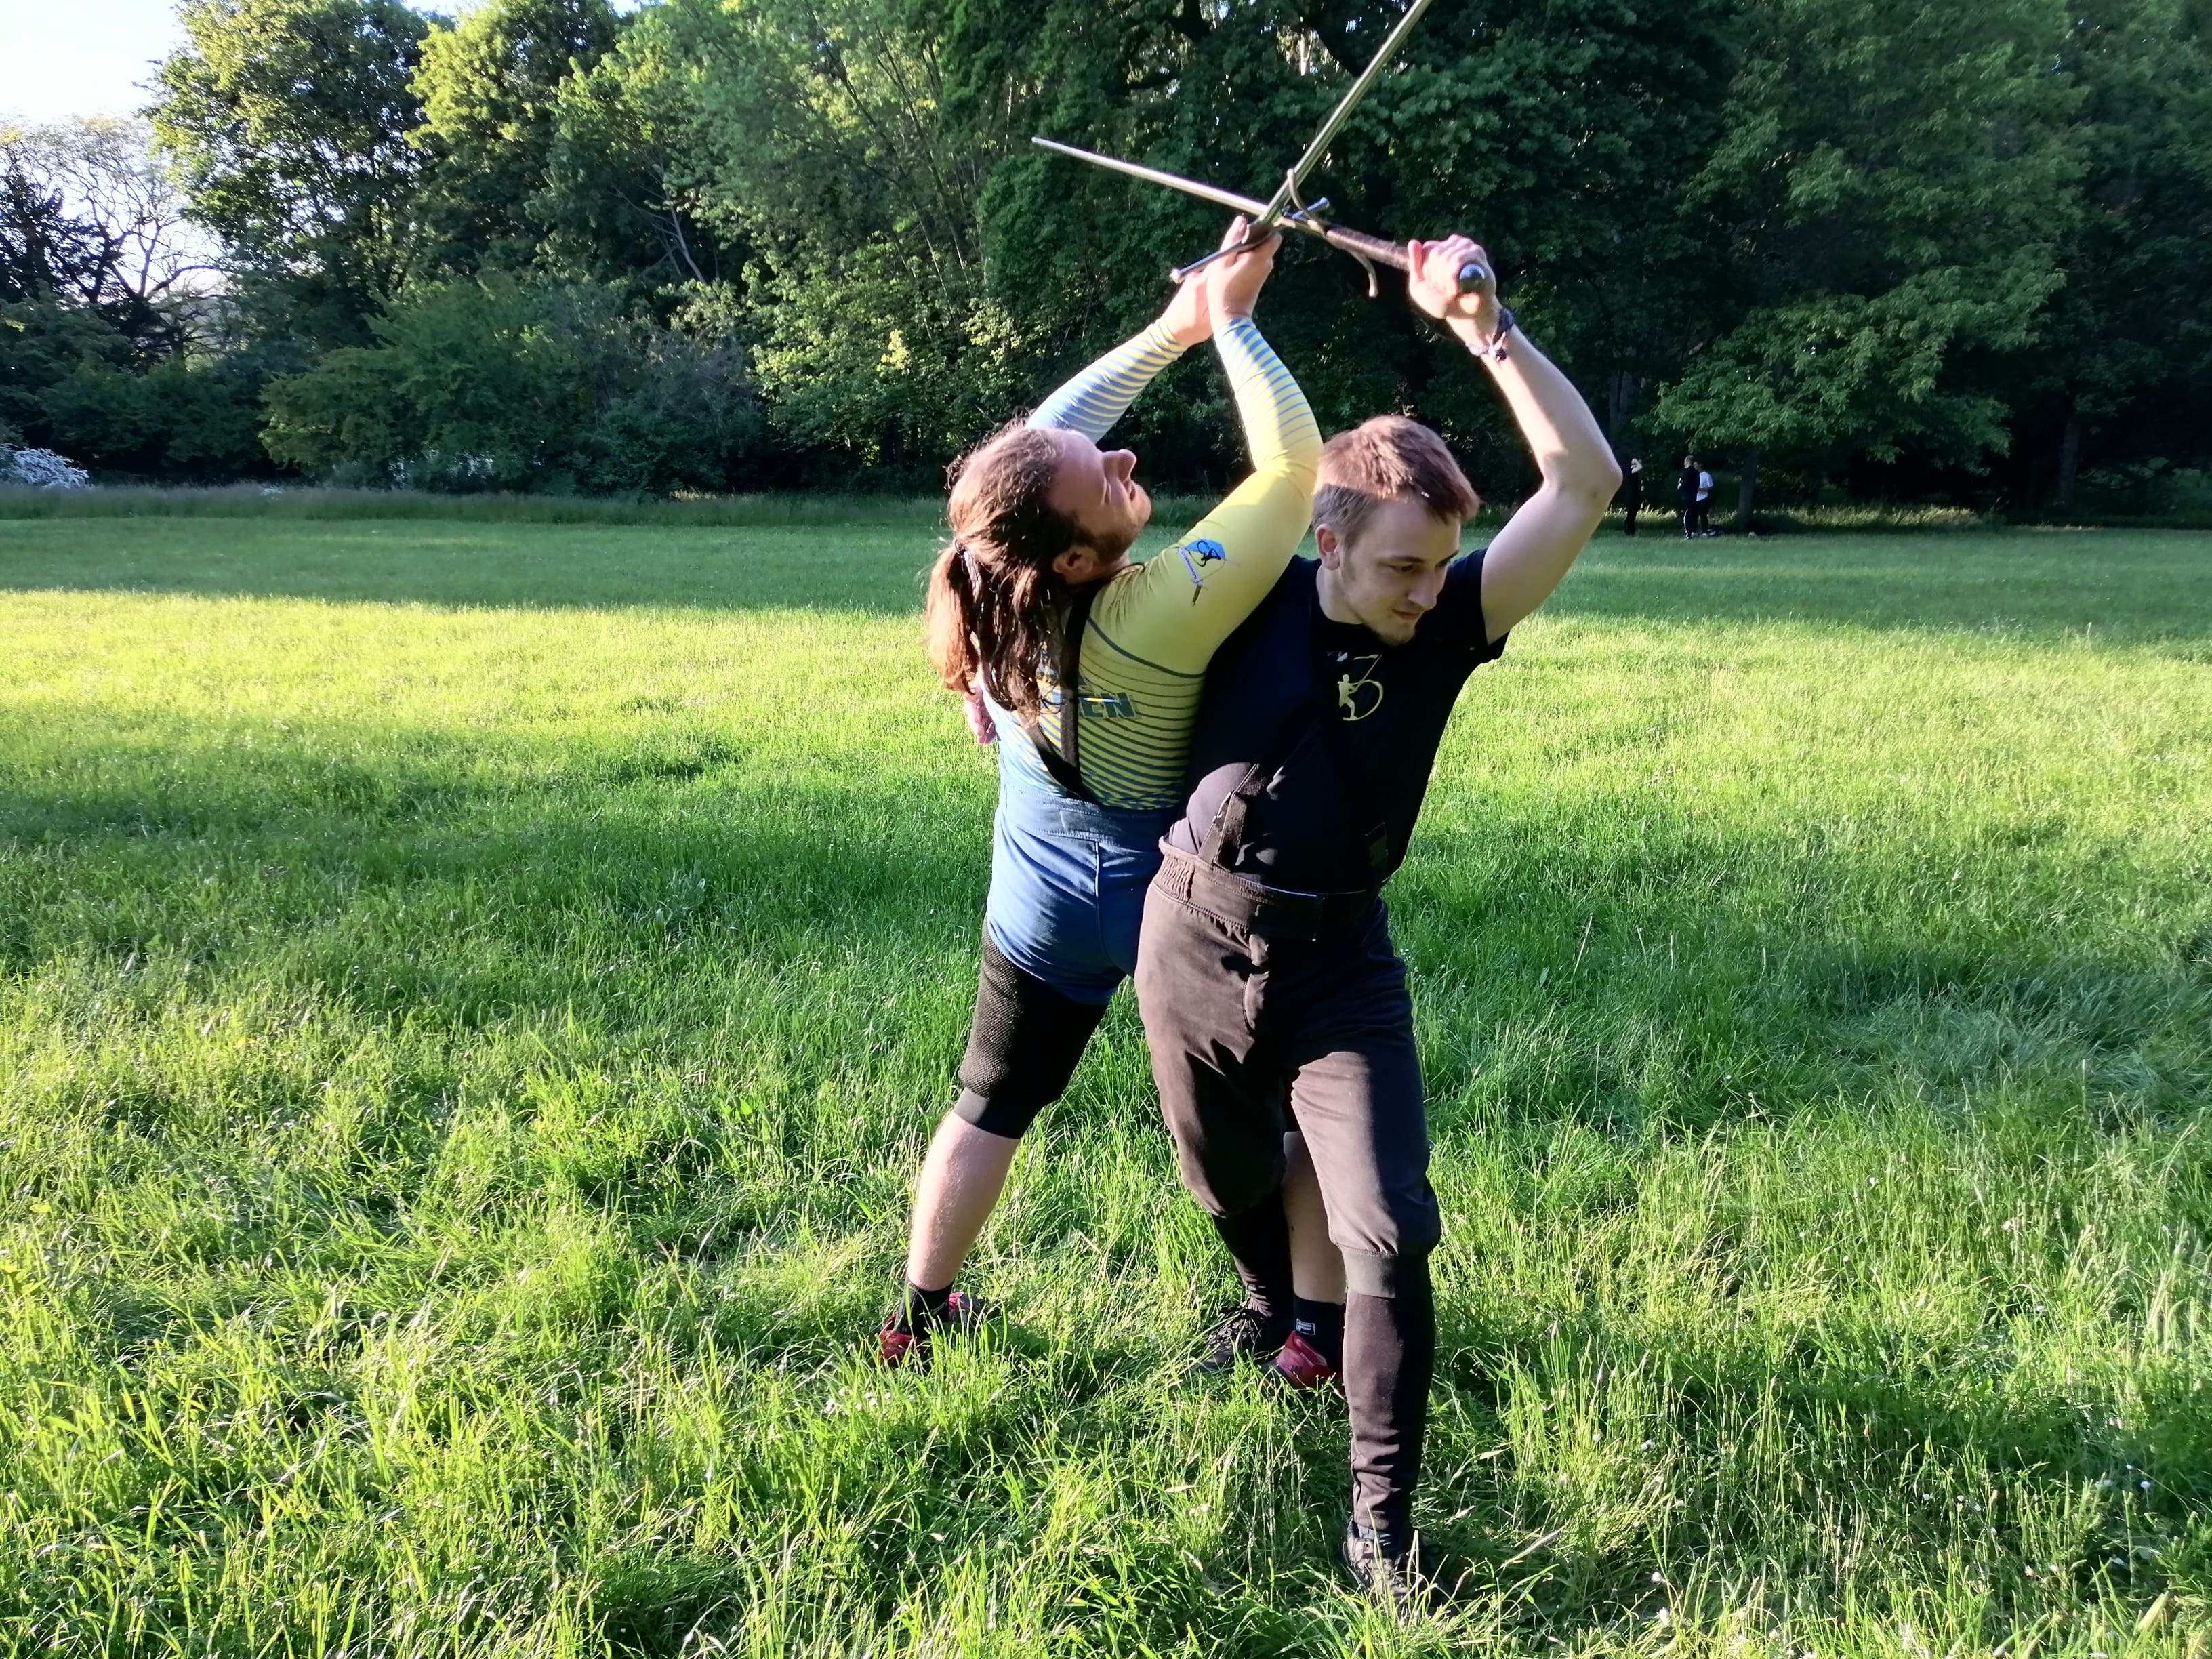
\includegraphics[scale=.05]{Ringe1.jpg}
    \caption{Das Leibringen}
    \label{fig:Leibringen}
\end{figure}

Der Körper des Gegenübers kann direkt angegriffen werden, Körperringstücke sind möglich.

\newpage

\subsubsection{Bindung}\label{Bindung0}

Die Bindung (oder das Band) beschreibt das Verhalten zweier sich berührender Klingen. Das Aufeinandertreffen der Klingen wird als Anbinden bezeichnet.
\\
\\
Lässt sich das Schwert des Gegenübers nach dem Aufeinandertreffen verdrücken, ist dies eine weiche oder schwache Bindung. Wird man hingegen selbst verdrückt oder kann das Schwert des Gegenübers selbst nicht bewegen, spricht man von einer harten oder starken Bindung.
\\
\\
Allgemein ist eine Bindung von oben über die Klinge des Gegners stärker. Eine Bindung mit Schneider auf Fläche hat in der Regel ebenfalls einen Vorteil.
\\
\\
Die Geometrie und das Kräfteverhältnis im Band werden zudem durch die Stelle der Anbindung bestimmt. Da scharfe Klingen in der Regel aneinenader haften (oder ''beißen''), erhält sich dieses Klingenverhältnis bis es aktiv aufgelöst oder geändert wird.
\\
\\
Liegt man mit der eigenen Schwäche in der Stärke des:der Gegner:in, hat diese:r einen starken Karftvorteil. Gleiches gilt auch umgekehrt.
\\
\\
Von einer ''neutralen Bindung'' wird gesprochen, wenn beide Klingen mittig und ohne erkennbaren geometrischen Vorteil anbinden.

\subsubsection{Vor, Nach und Indes}

Der Begriff ''Tempo'' beschreibt im historischen Fechten das zeitliche Verhältnis zweier Fechter:innen oder dient als ''zeitliche Einheit'' für fechterische Aktionen.
\\
\\
Besitzt man die Initiative und zwingt so den:die Gegner:in zum versetzen, so ficht man aus dem ''Vor''. Behält man das ''Vor'', so gibt man dem:der Gegner:in keine Möglichkeit, selbst Aktionen zu beginnen, so lange diese:r auf Eigenschutz achtet.
\\
\\
Muss man jedoch selbst auf einen Angriff reagieren, und ficht aus der Versatzung schnell zur nächsten Blöße, so bricht man das ''Vor'' des:der Gegner:in mit dem eigenen ''Nach''.
\\
\\
Das ''Indes'' liegt zwischen ''Vor'' und ''Nach''. Es beschreibt eine Aktion, die während der eines:einer Gegner:in ausgeführt wird.
\\
\\
Grundsätzlich ist es immer vorteilhaft, sich im ''Vor'' zu befinden, das heißt im Kampf die Initiative zu besitzen. Auf ein gegnerisches "Vor" wird im Idealfall mit einem eigenen "Indes" geantwortet, um dieses zu brechen.

\subsection{Fechterische Grundprinzipien}

Alle von den Fechtmeistern beschriebenen Stücke folgen grundlegenden Prinzipien. Diese sind zwar meist nicht explizit beschrieben und doch ziehen sich ähnliche Muster, Annahmen und Regeln wie ein roter Faden über die Autoren und Bücher hinweg durch alle Quellen. Nachfolgend wurden deshalb einige Grundlegende Prinzipien zusammengetragen, welche alle Fechtenden für das Interpretieren neuer Stücke verinnerlichen und anwenden sollten. Häufig können diese Prinzipien auch als Ziele eines Fechtstücks begriffen werden. Sollen mehrere Ziele gleichzeitig erfüllt werden kann es natürlich vorkommen, dass ein Interessenkonfilkt bei der Erfüllung der Ziele entsteht. In diesem Falle sollte die Interpretation den bestmöglichen Kompromiss für die Erfüllung aller Ziele bieten.

\subsubsection{Eigenschutz}

Die meisten Quellen mit Bezug zum Langen Schwert oder zum Langen Messer befassen sich mit dem sogenannten „Blossfechten“ also dem Fechten ohne jegliche Schutzausrüstung. In diesem Kontext wird ein Treffer sehr wahrscheinlich fatale Konsequenzen für den Getroffen haben. Aus diesem Grund hat der Eigenschutz  immer höchste Priorität.
\\
\\
Eigenschutz kann durch mehrere Wege erreicht werden:

\begin{enumerate}[I.]
    \item Bewegung der eigenen Waffe zur Gefahrenquelle
    \item Bewegung der Füße/Beine um sich aus dem Gefahrenbereich (häufig der Schnittlinie eines Schwertes) zu bewegen, bspw. durch Austreten zur Seite
    \item Bewegung des Körpers um sich aus dem Gefahrenbereich zu bewegen, bspw. durch Verlagern des Oberkörpers hinter die Bewegungslinie des eigenen Schwertes
    \item Bewegung der gegnerische Waffe vom eigenen Körper weg; Dies kann durch eigene Motivation oder aber durch den:die Gegner:in selbst geschehen, bspw. wenn diese:r sich verschätzt
\end{enumerate}

\newpage

\subsubsection{Häue, Schnitte, Stiche - Die drei Wunder}

\paragraph{Häue}

Häue sind die klassischste und für viele die intuitivste Angriffsform mit dem langen Schwert. Ein effektiver Hau kann auch mit wenig Kraft geschlagen werden, sollte aber ausreichend Weg zur Beschleunigung ($\sim$30cm) haben, bevor er sein Ziel trifft. Ein Hau kann automatisch Selbstschutz herstellen, wenn er in die gedeckte Bindung geschlagen wird.
\\
\\
Oberhau:

\FloatBarrier

\begin{figure}[!htb]
\minipage{0.24\textwidth}
    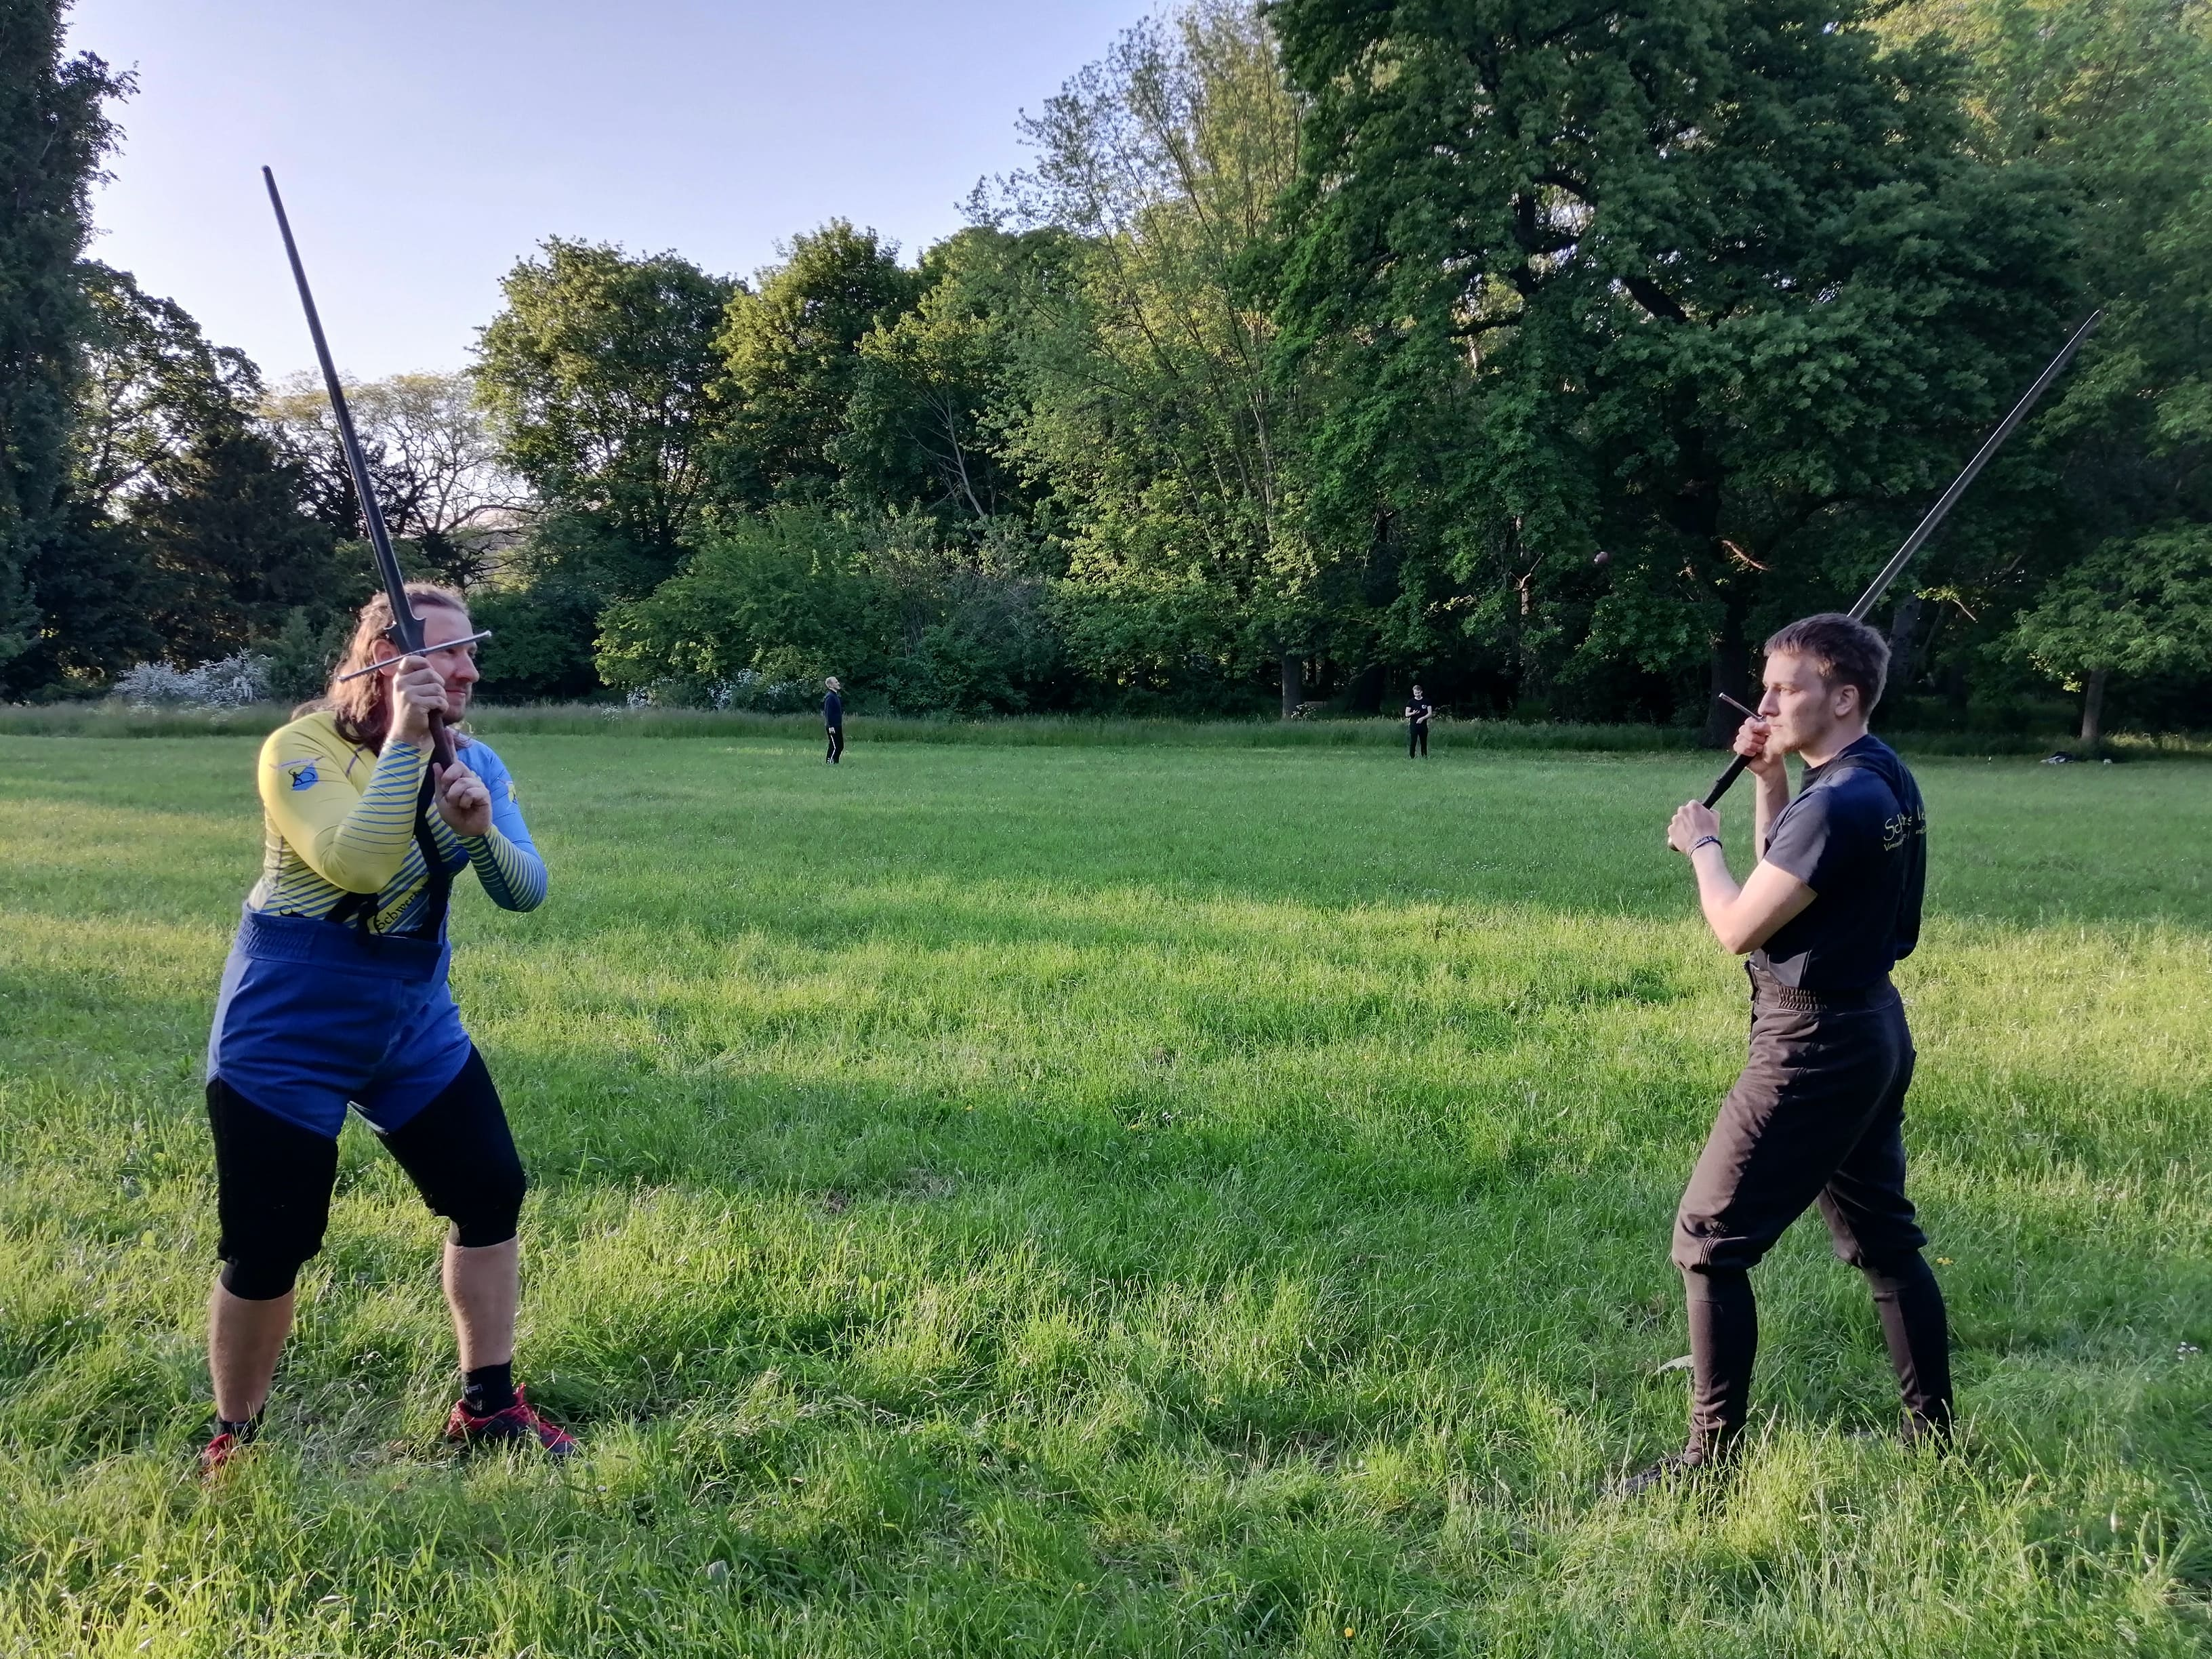
\includegraphics[width=\linewidth]{Oberhau1.jpg}
\endminipage\hfill
\minipage{0.24\textwidth}
    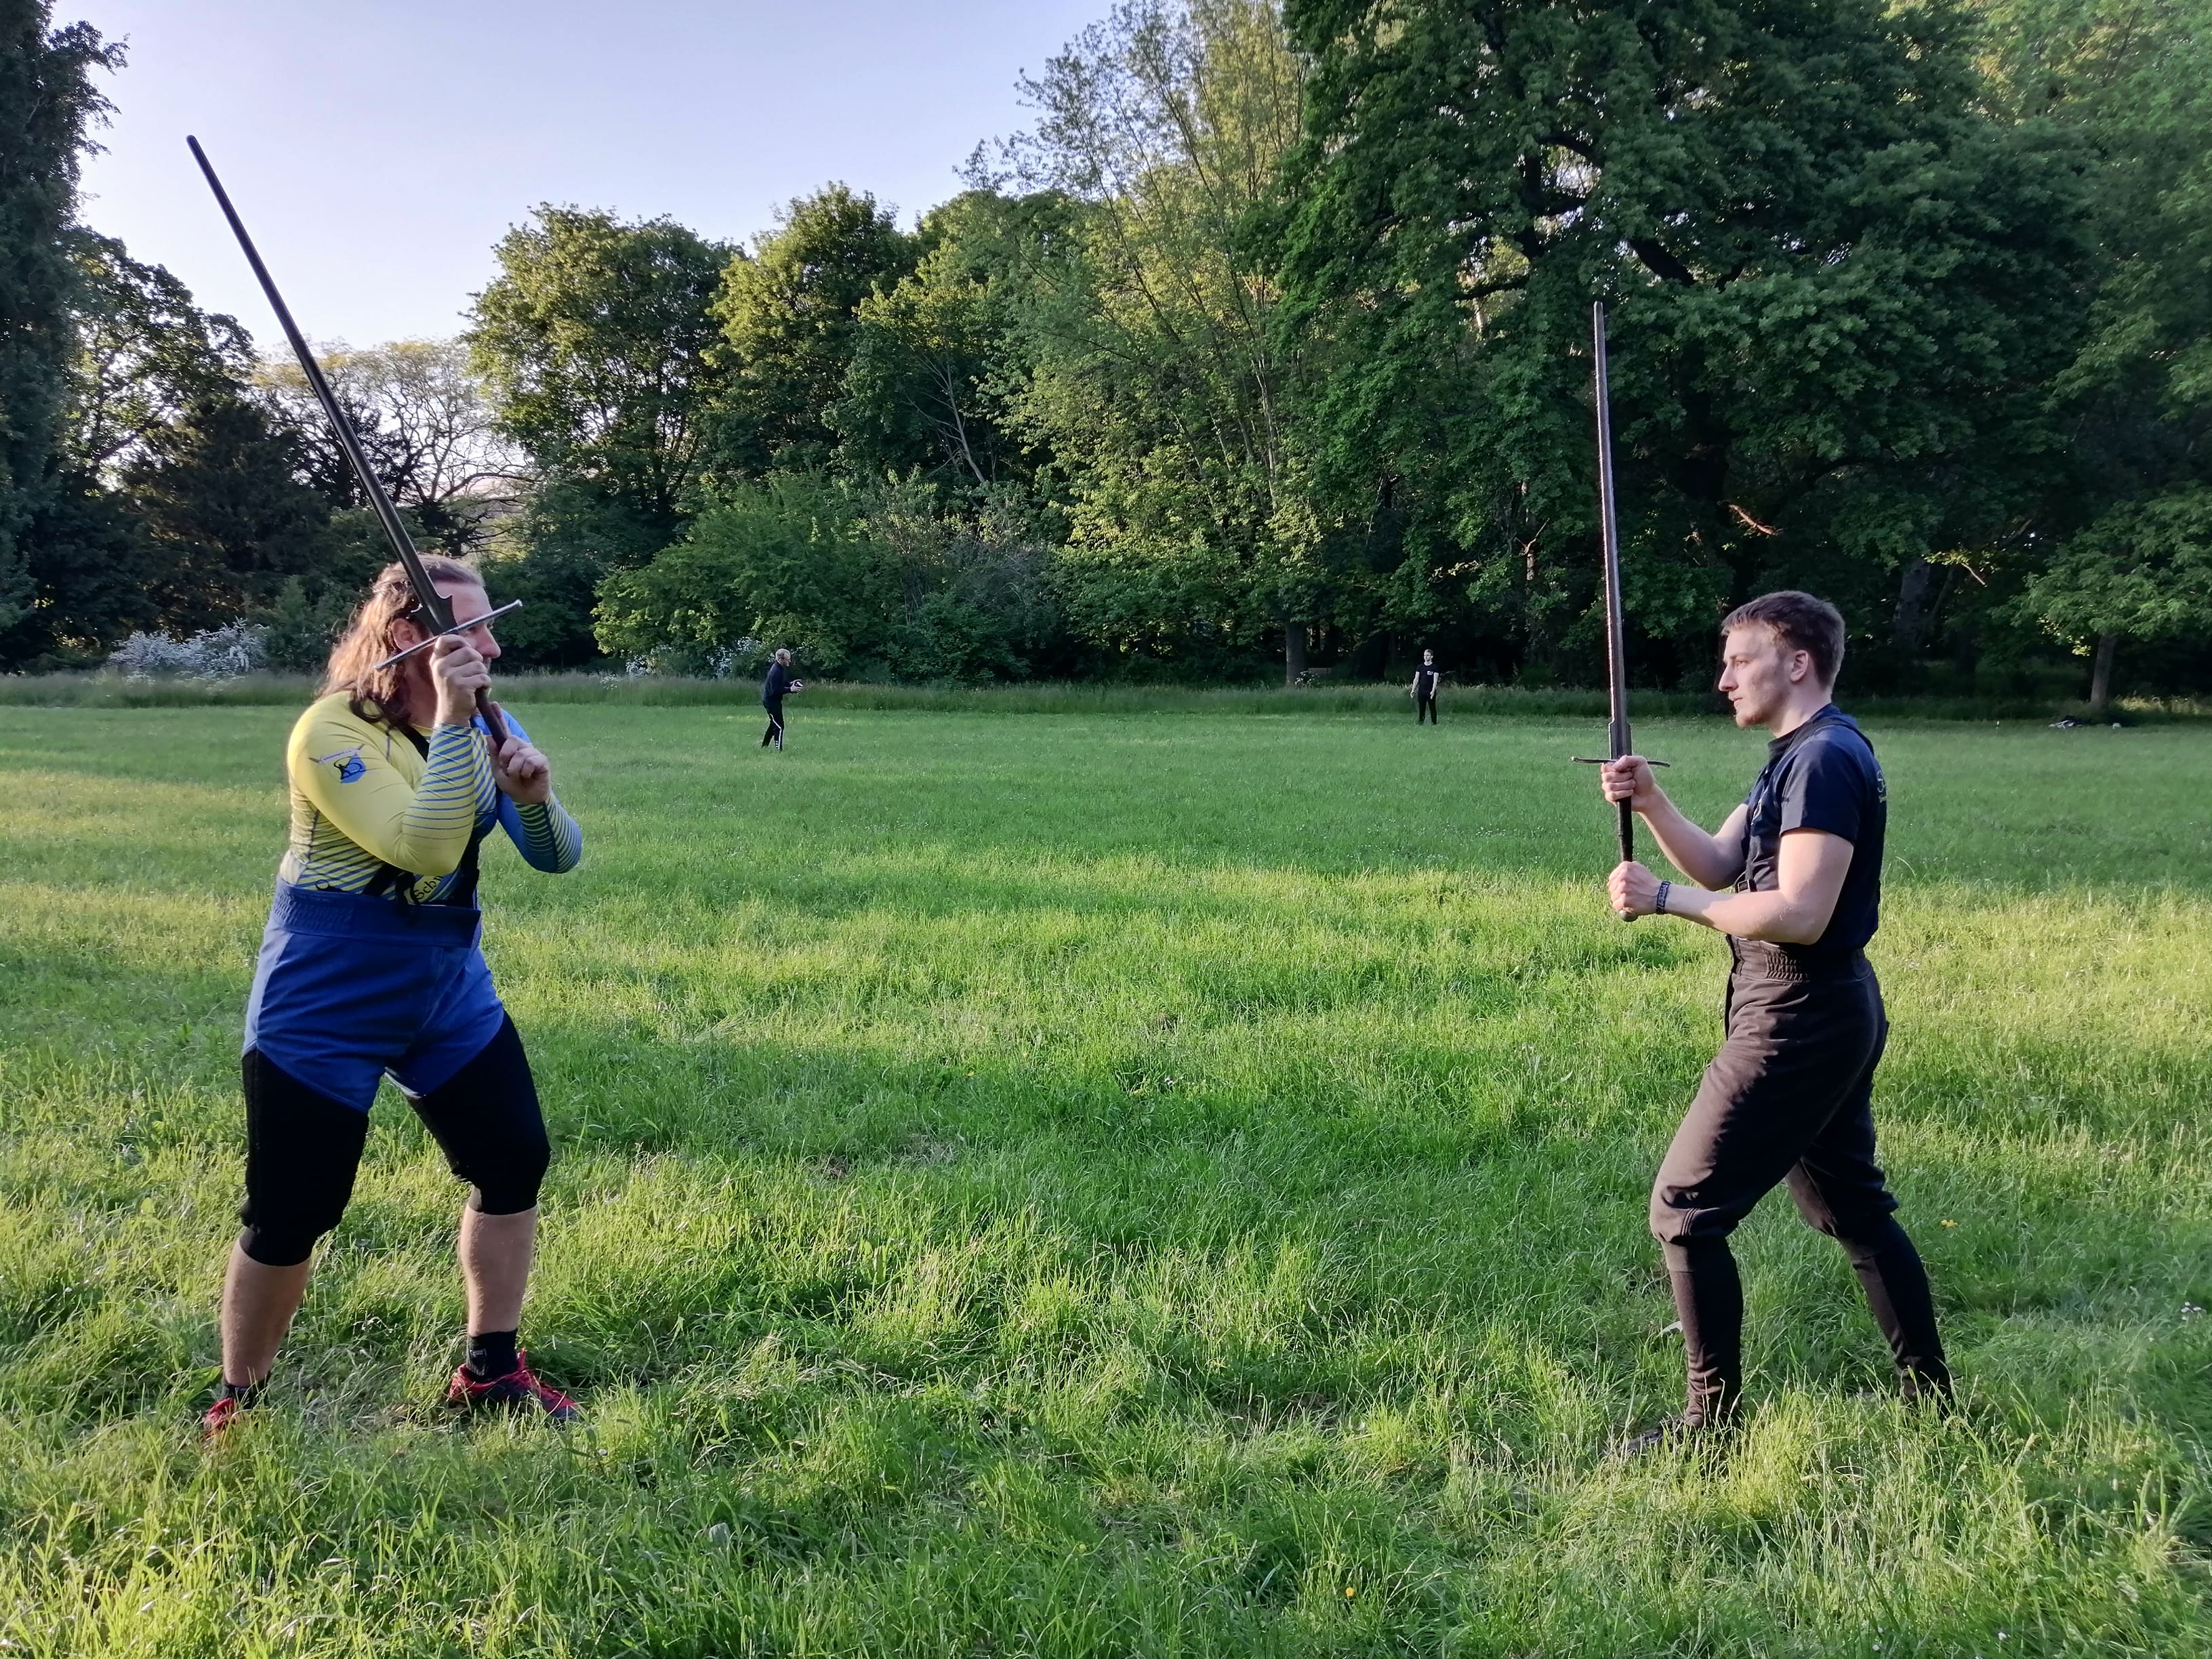
\includegraphics[width=\linewidth]{Oberhau2.jpg}
\endminipage\hfill
\minipage{0.24\textwidth}
    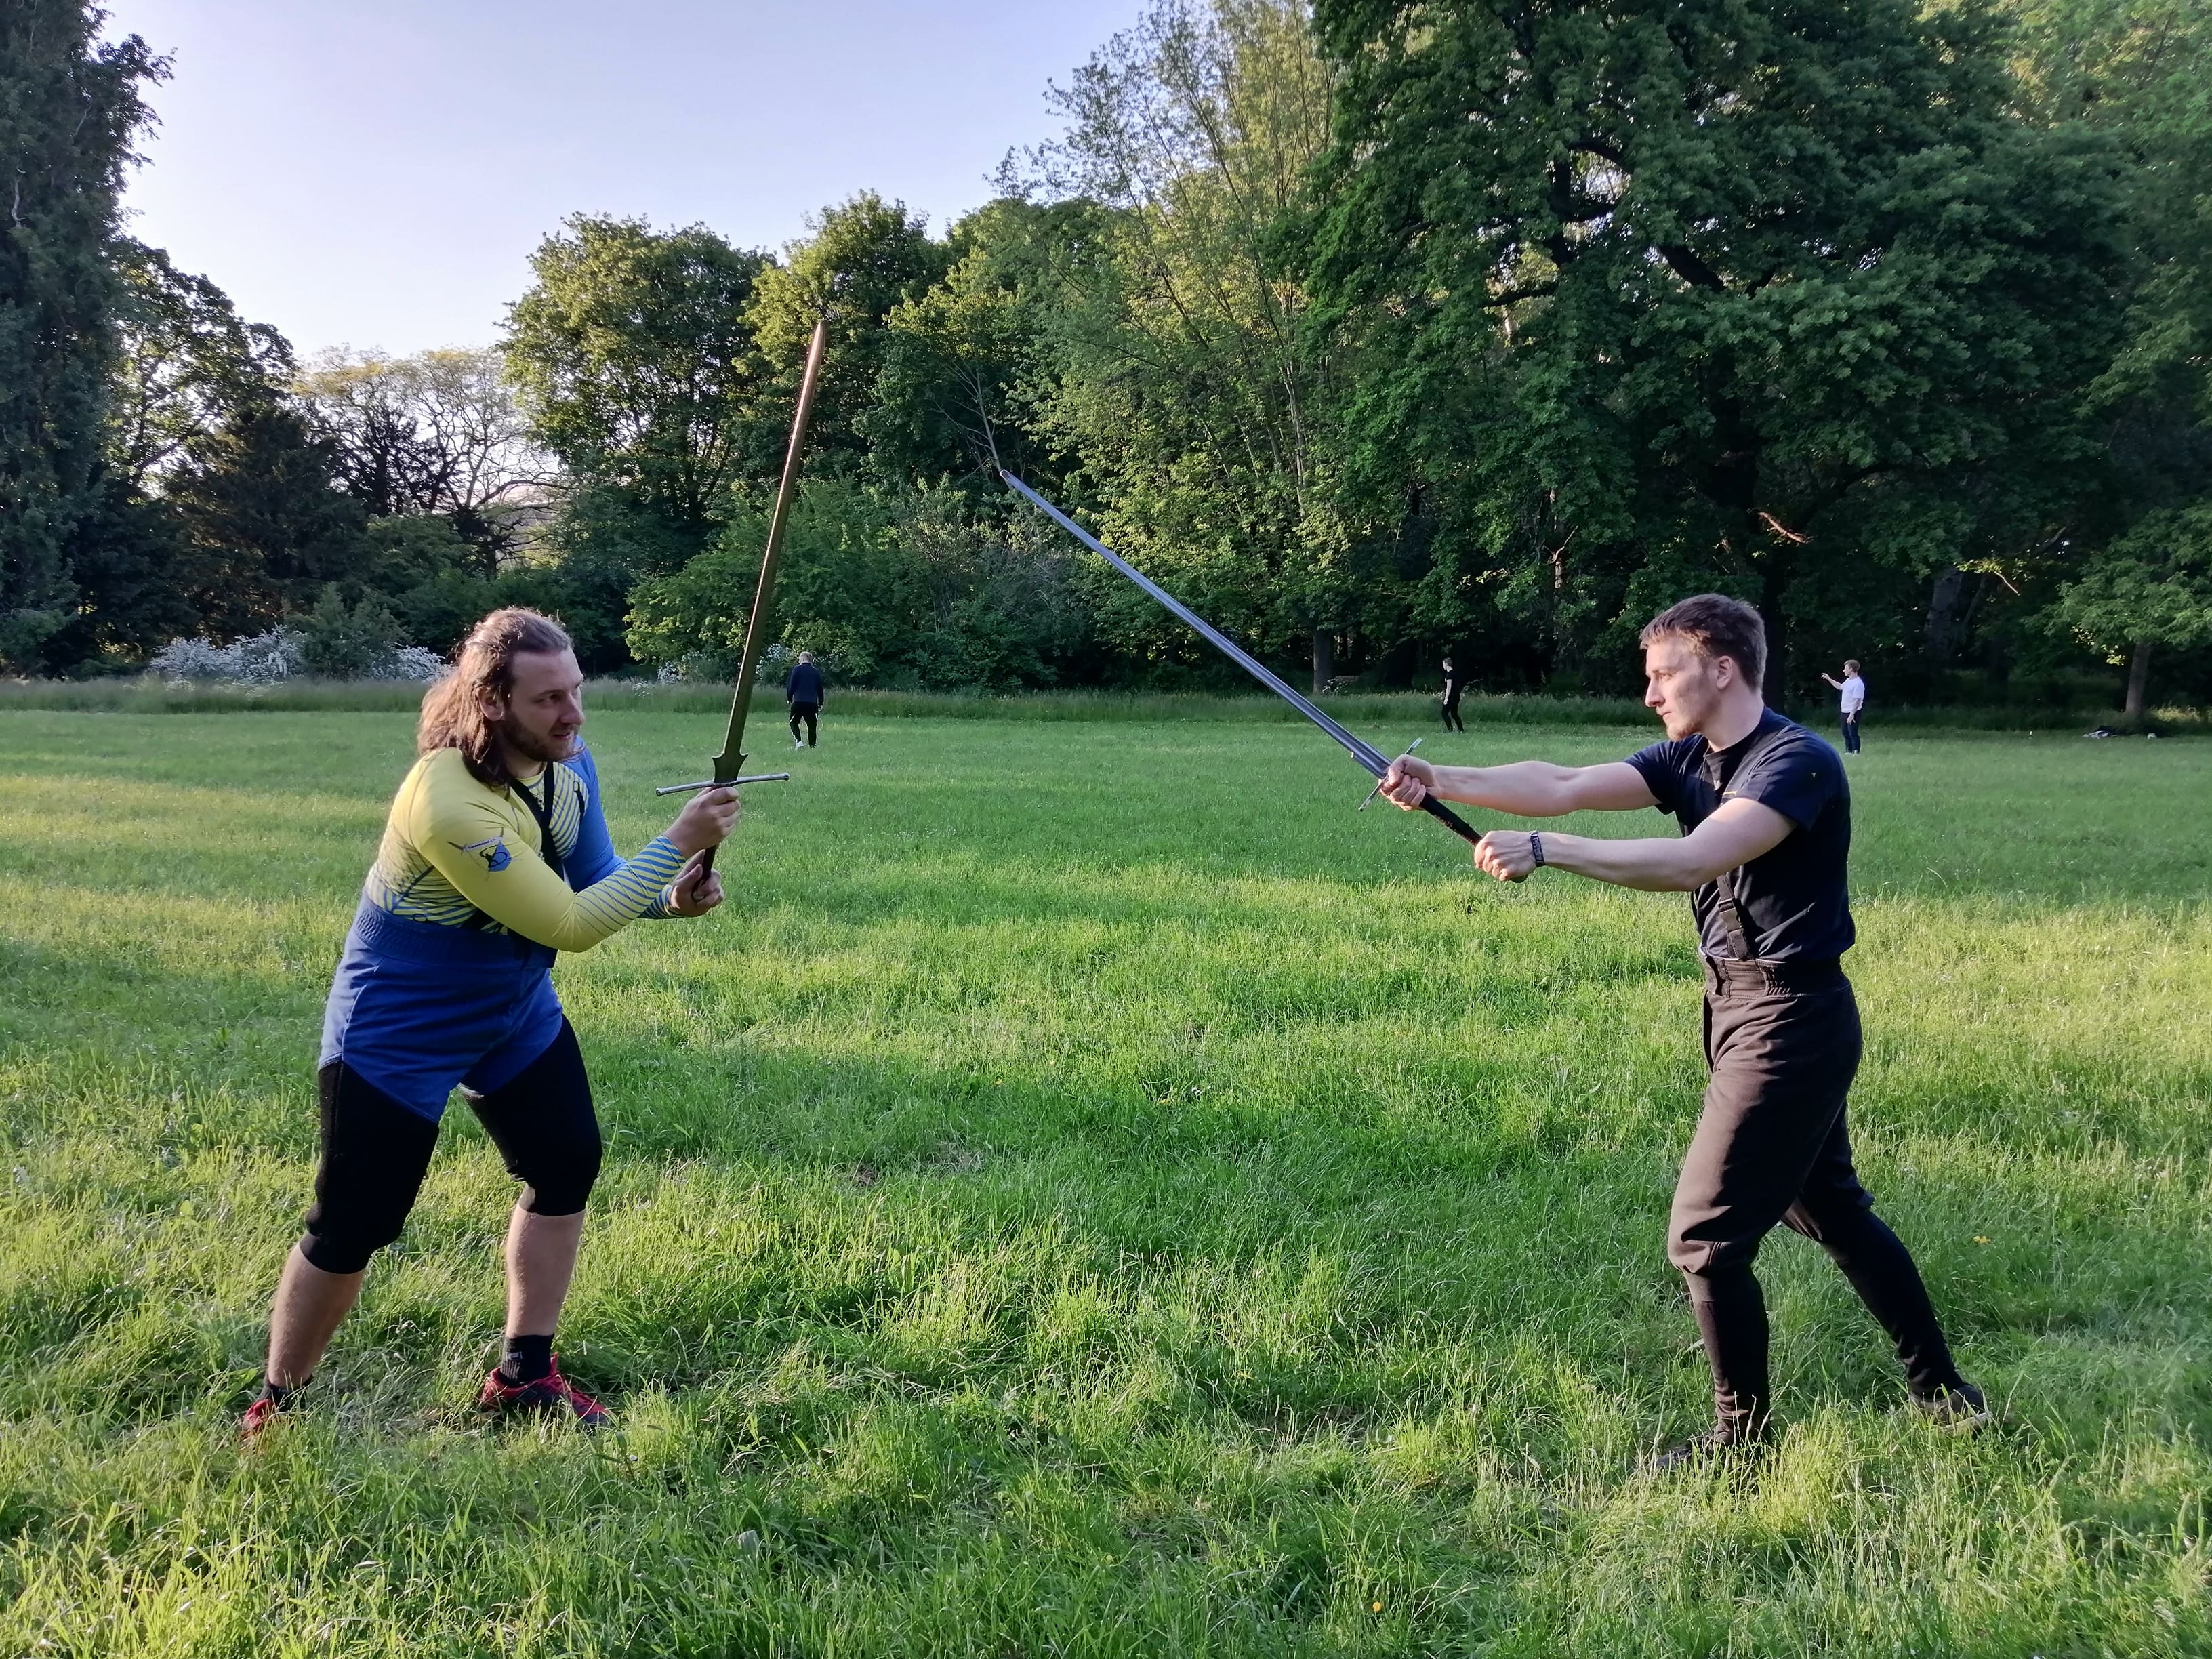
\includegraphics[width=\linewidth]{Oberhau3.jpg}
\endminipage\hfill
\minipage{0.24\textwidth}
    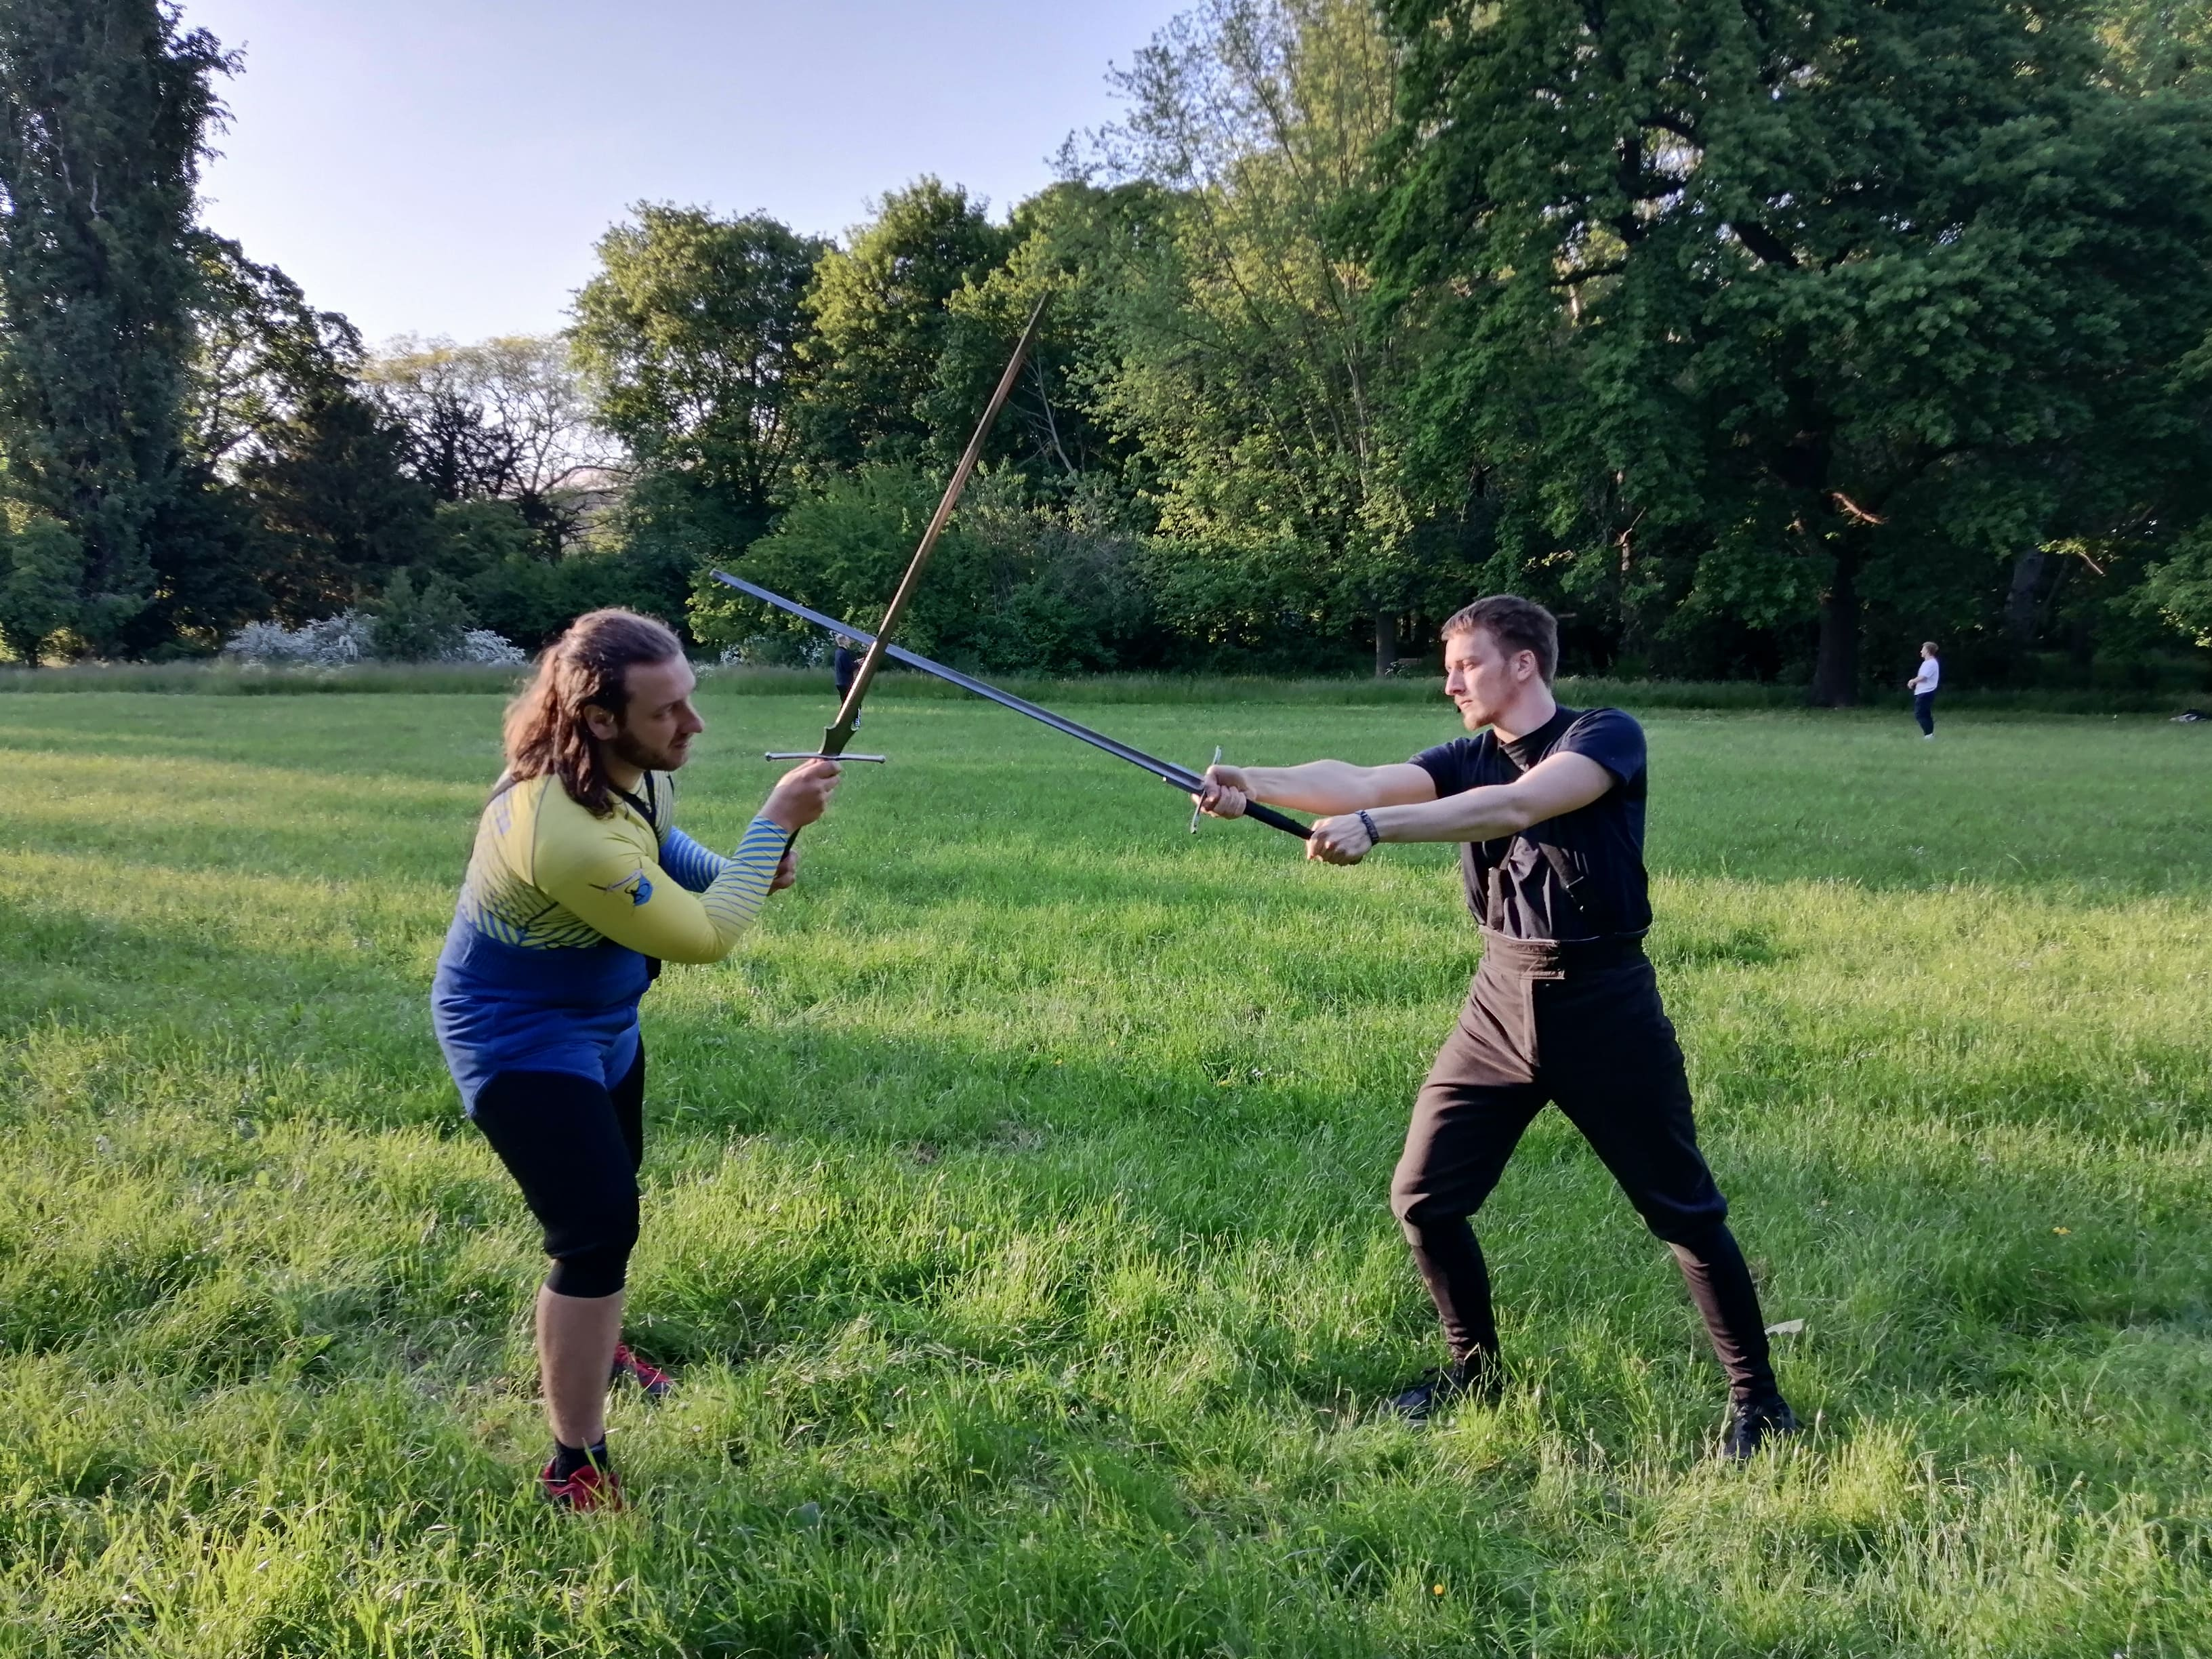
\includegraphics[width=\linewidth]{Oberhau4.jpg}
\endminipage
\end{figure}

\FloatBarrier
\hrule
\hfill
\\
Unterhau:

\FloatBarrier

\begin{figure}[!htb]
\minipage{0.24\textwidth}
    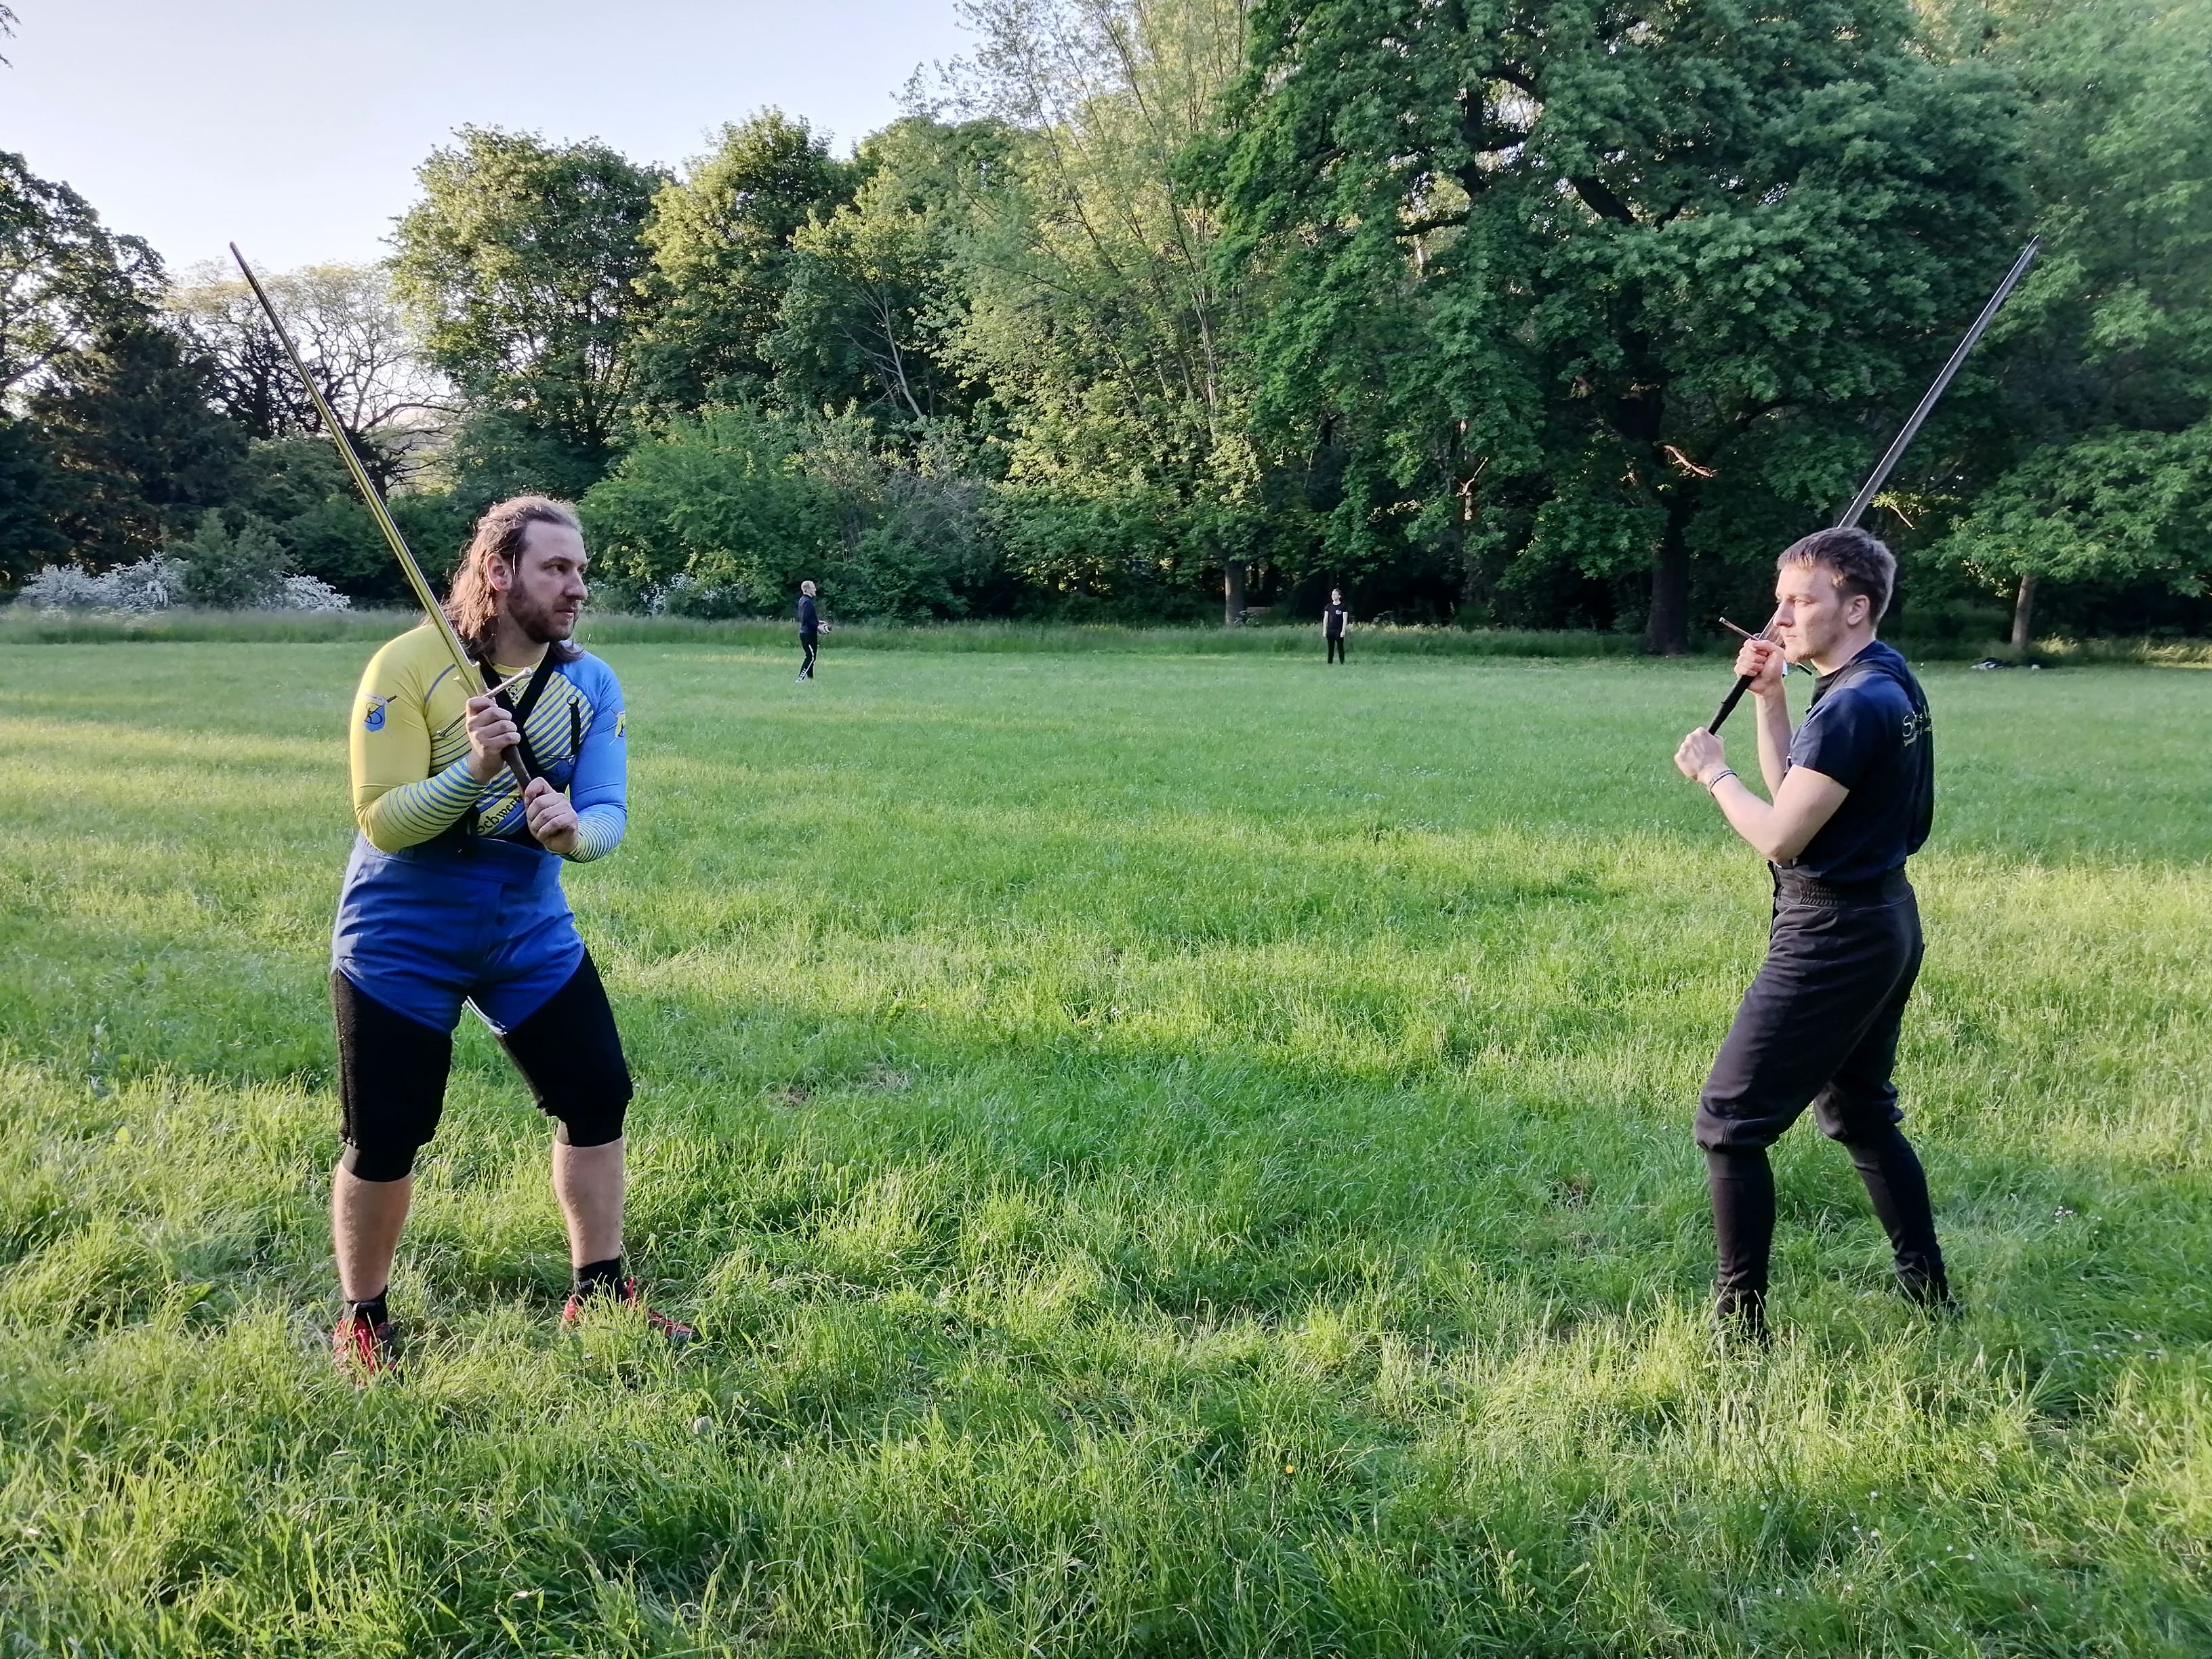
\includegraphics[width=\linewidth]{Unterhau1.jpg}
\endminipage\hfill
\minipage{0.24\textwidth}
    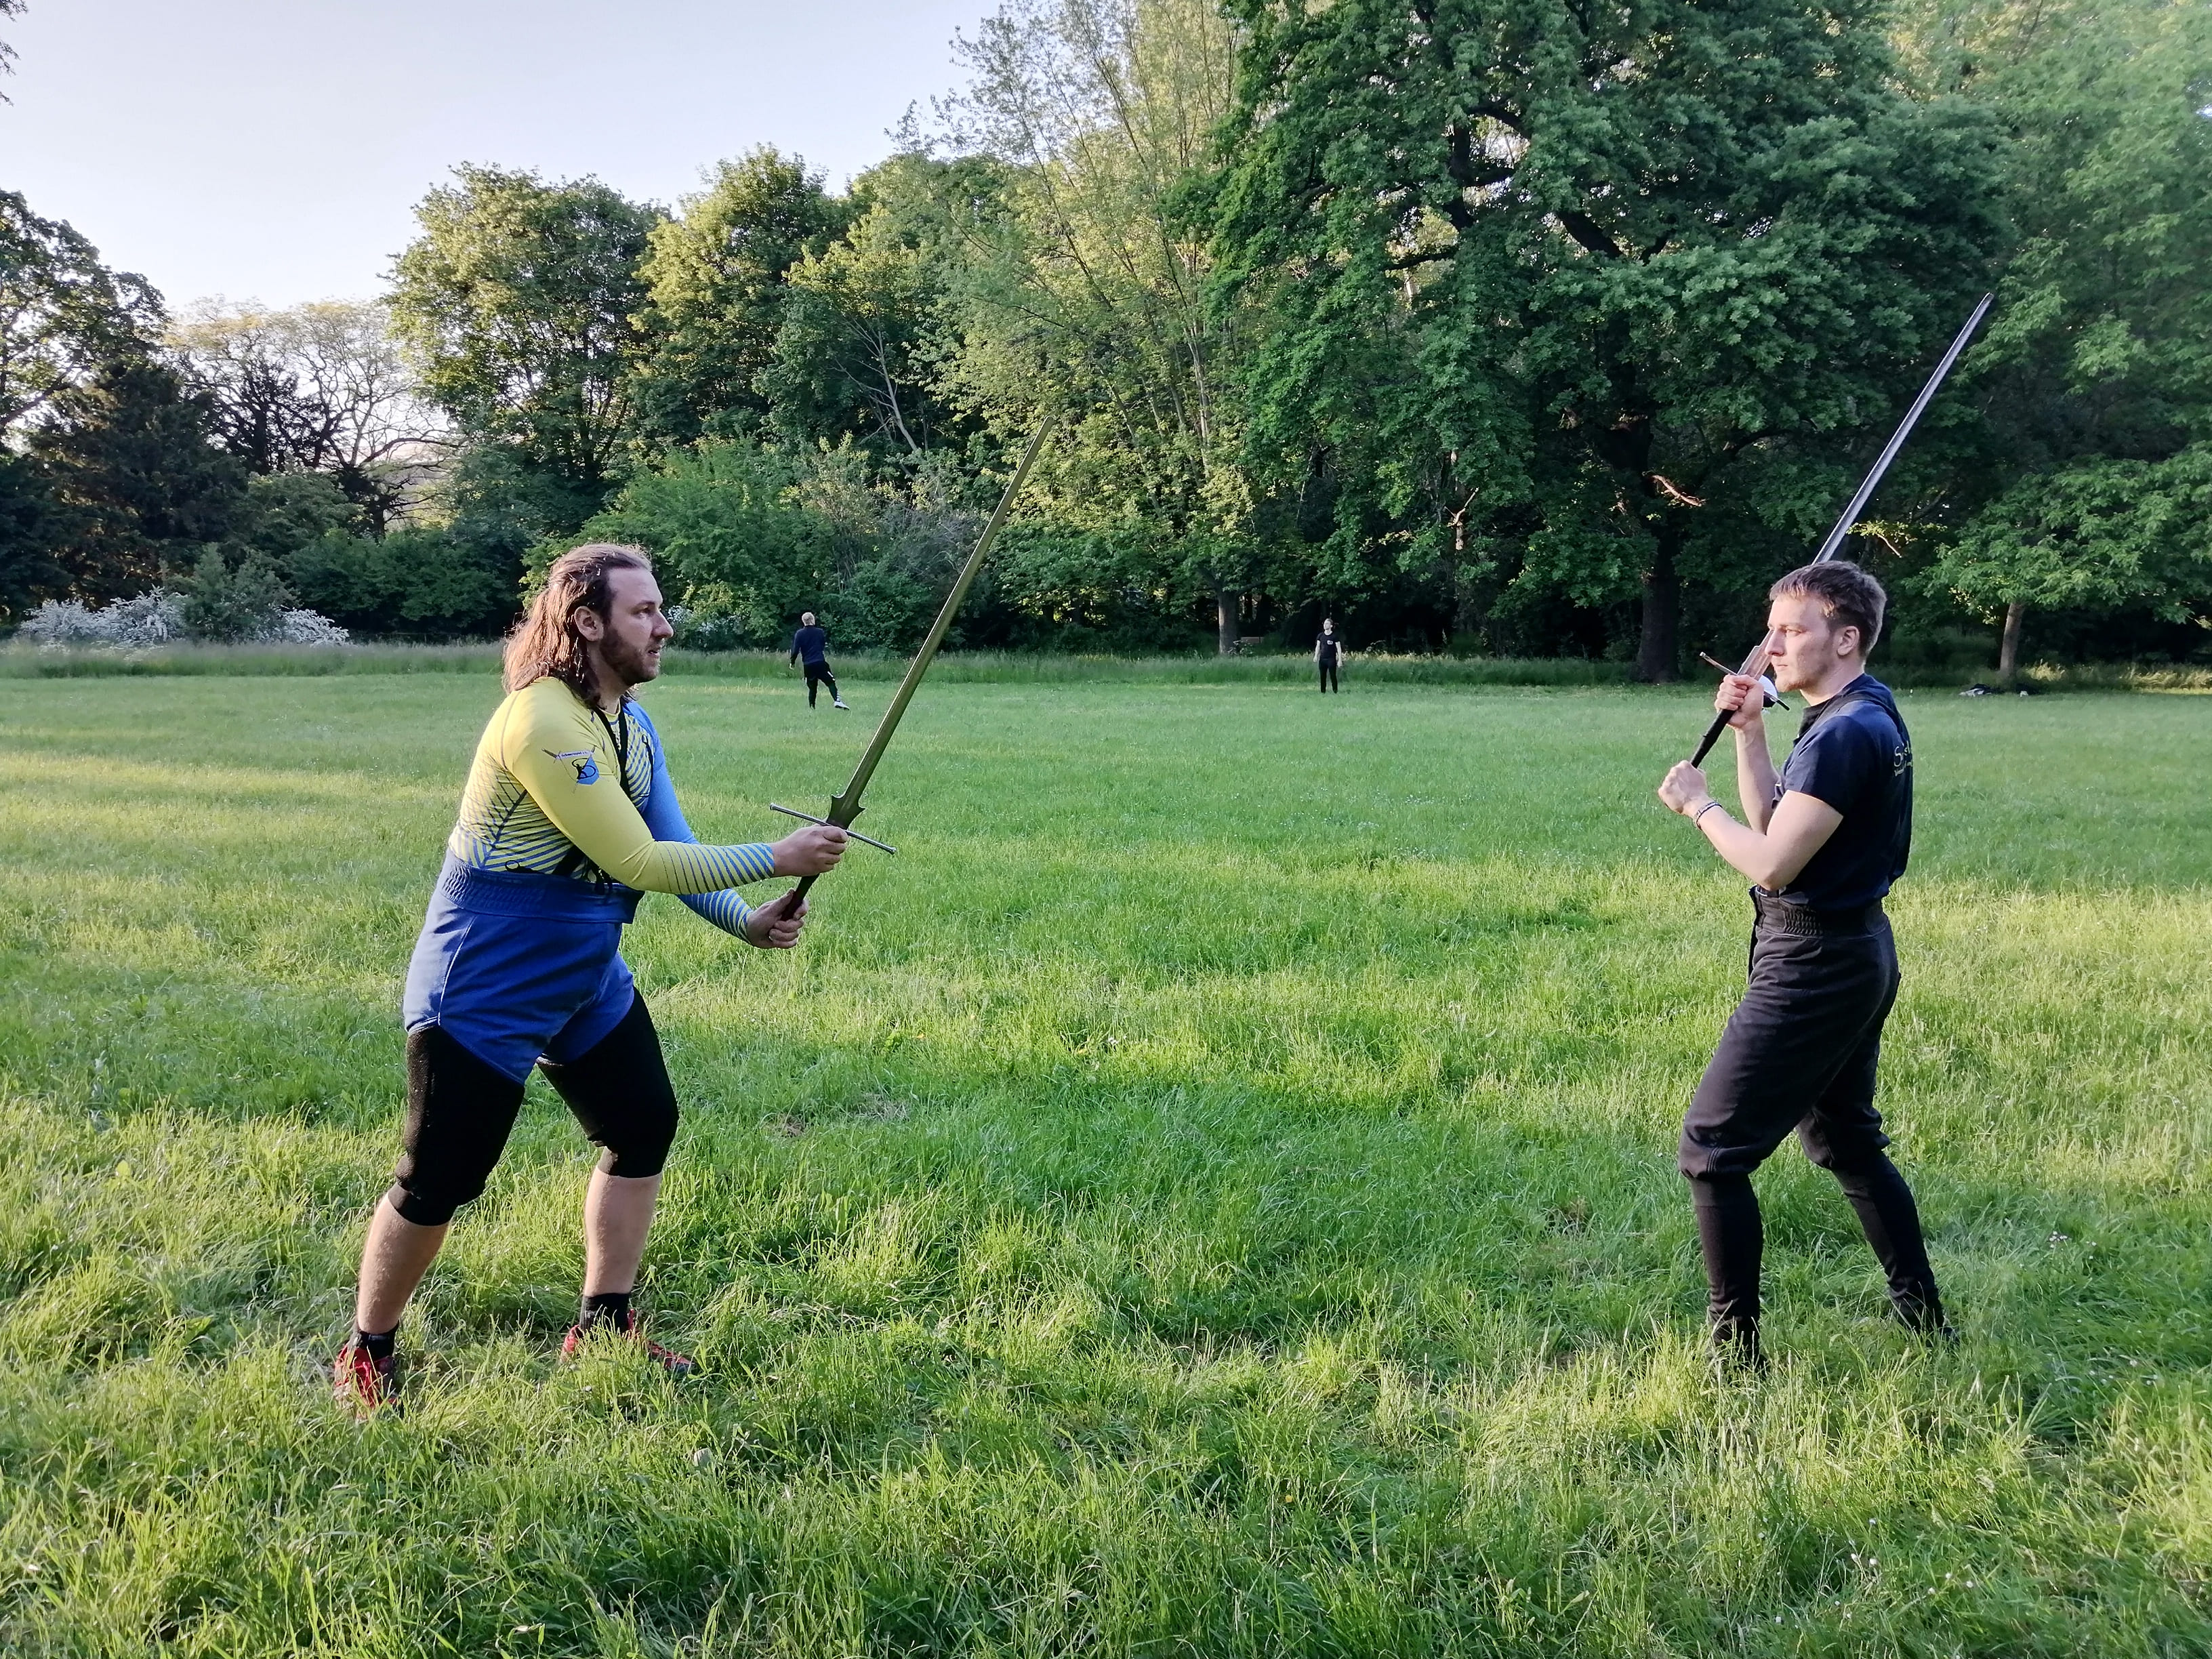
\includegraphics[width=\linewidth]{Unterhau2.jpg}
\endminipage\hfill
\minipage{0.24\textwidth}
    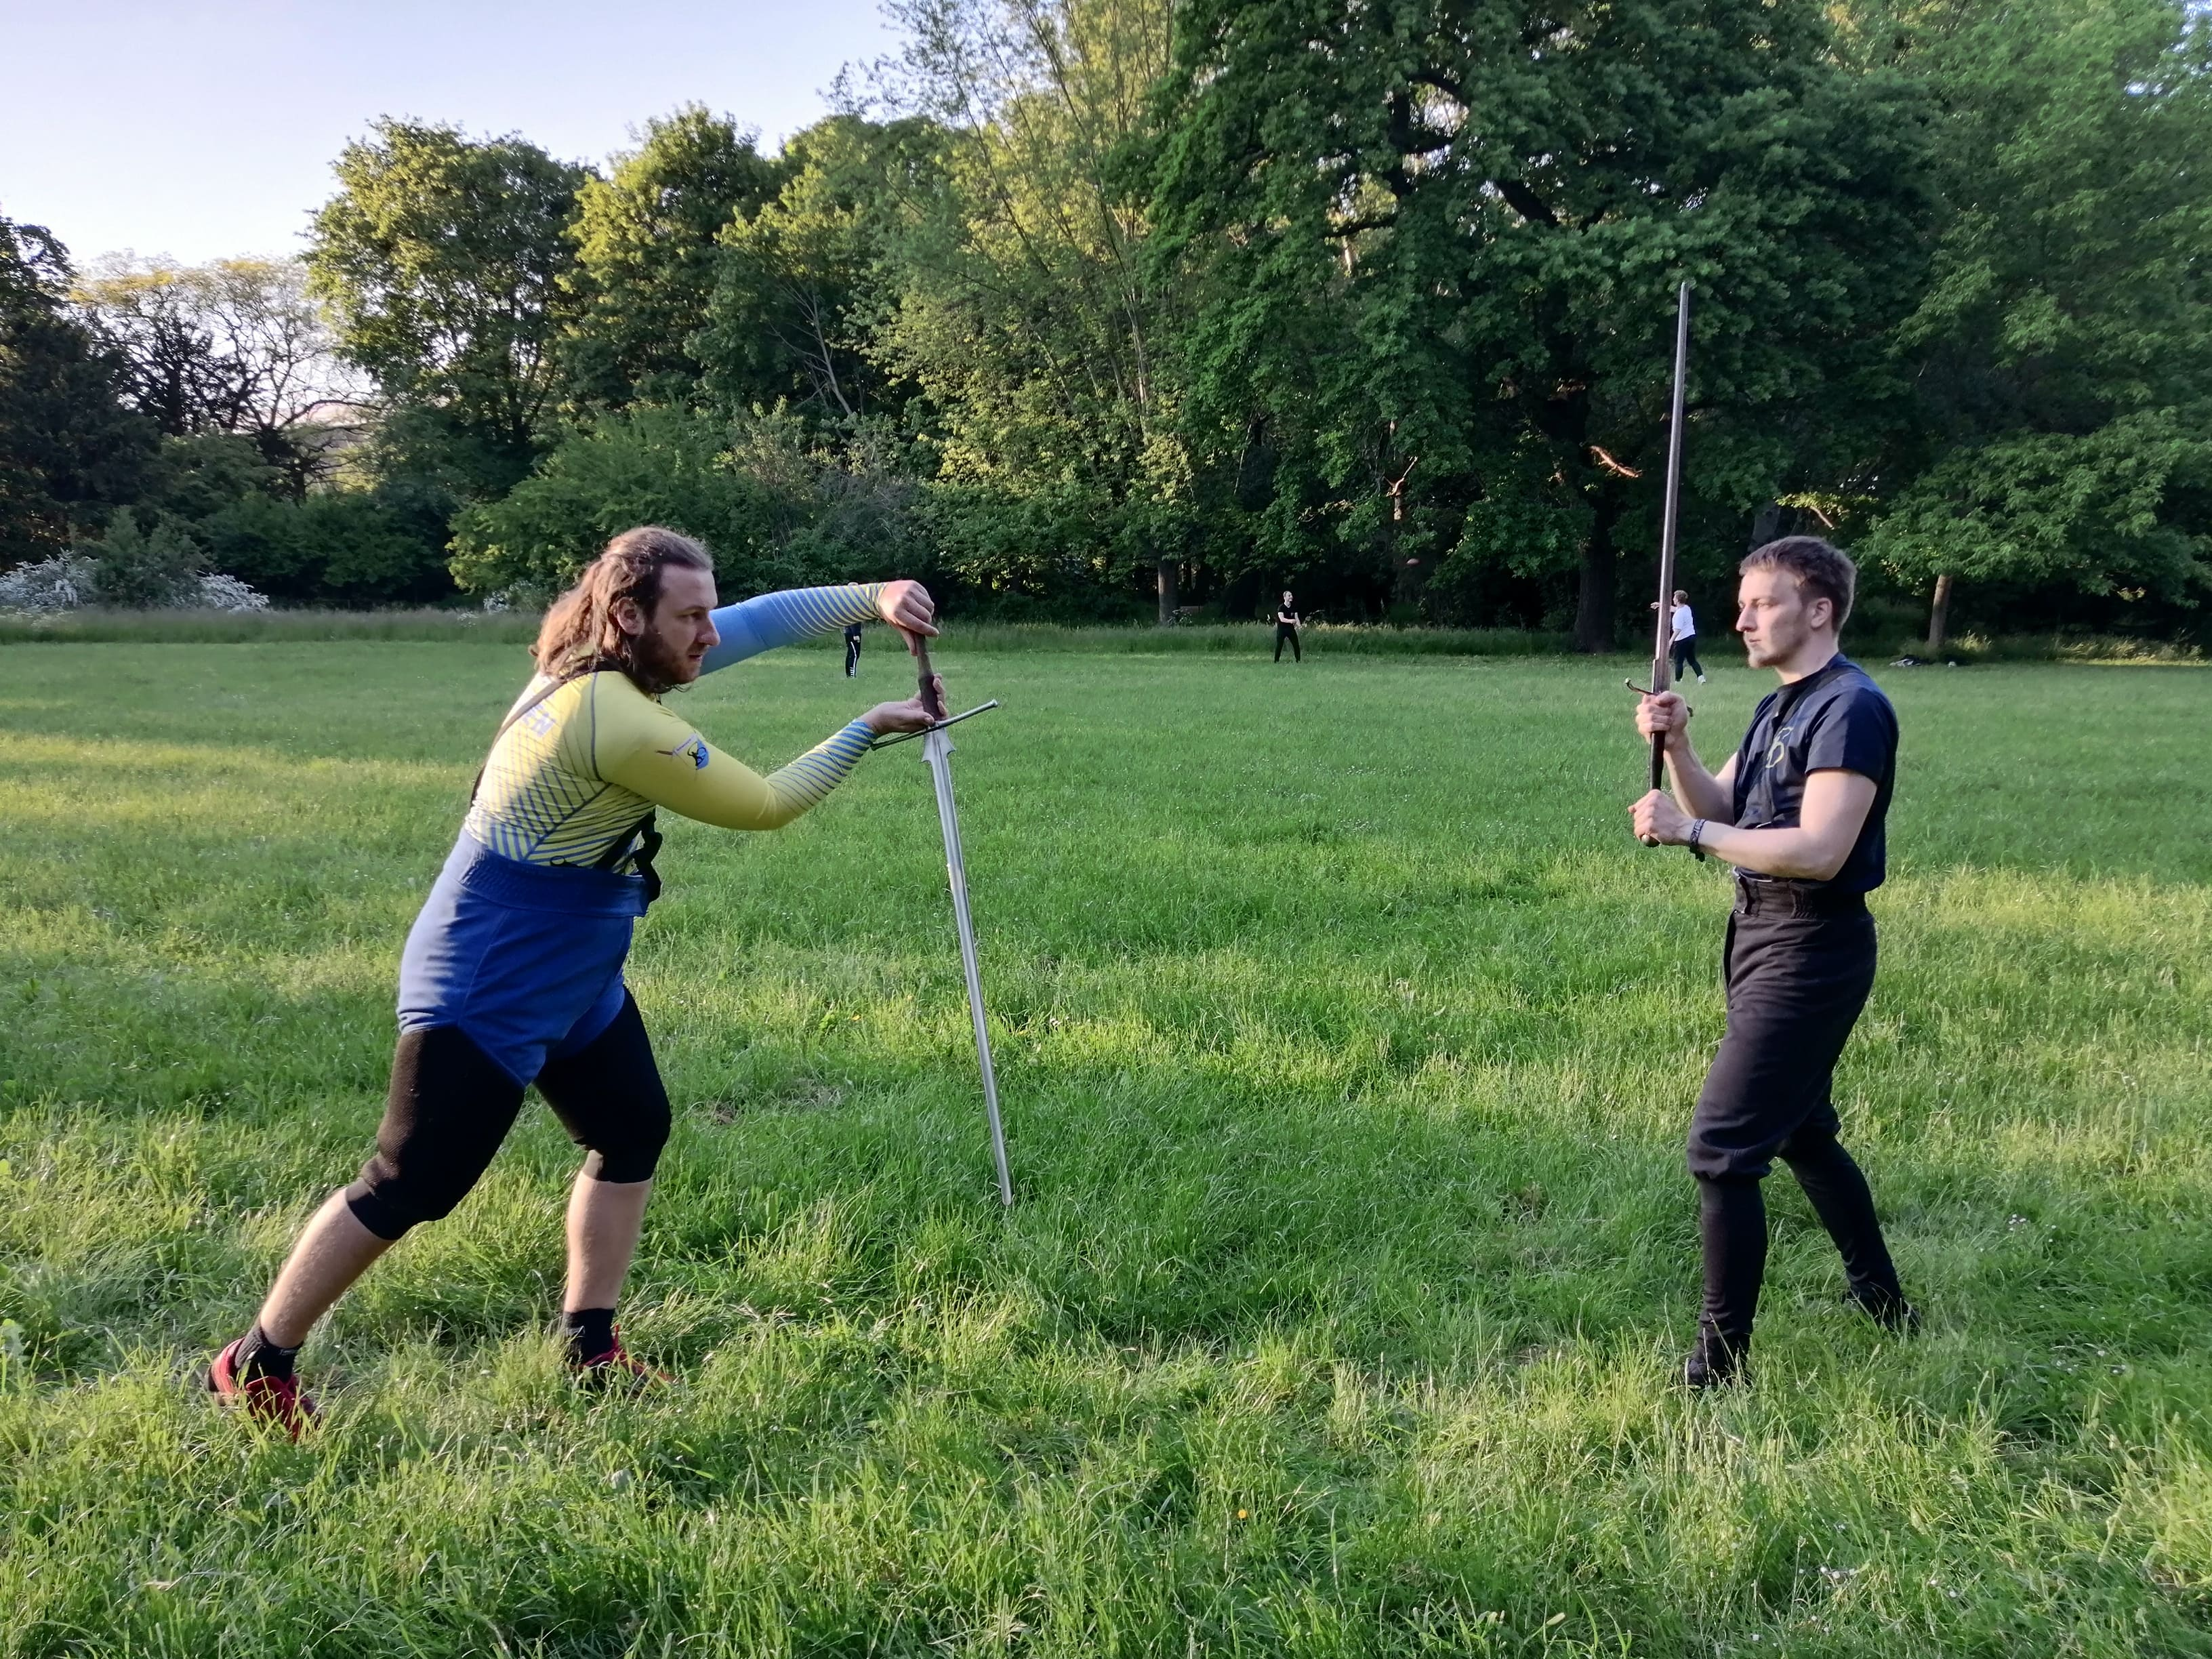
\includegraphics[width=\linewidth]{Unterhau3.jpg}
\endminipage\hfill
\minipage{0.24\textwidth}%
    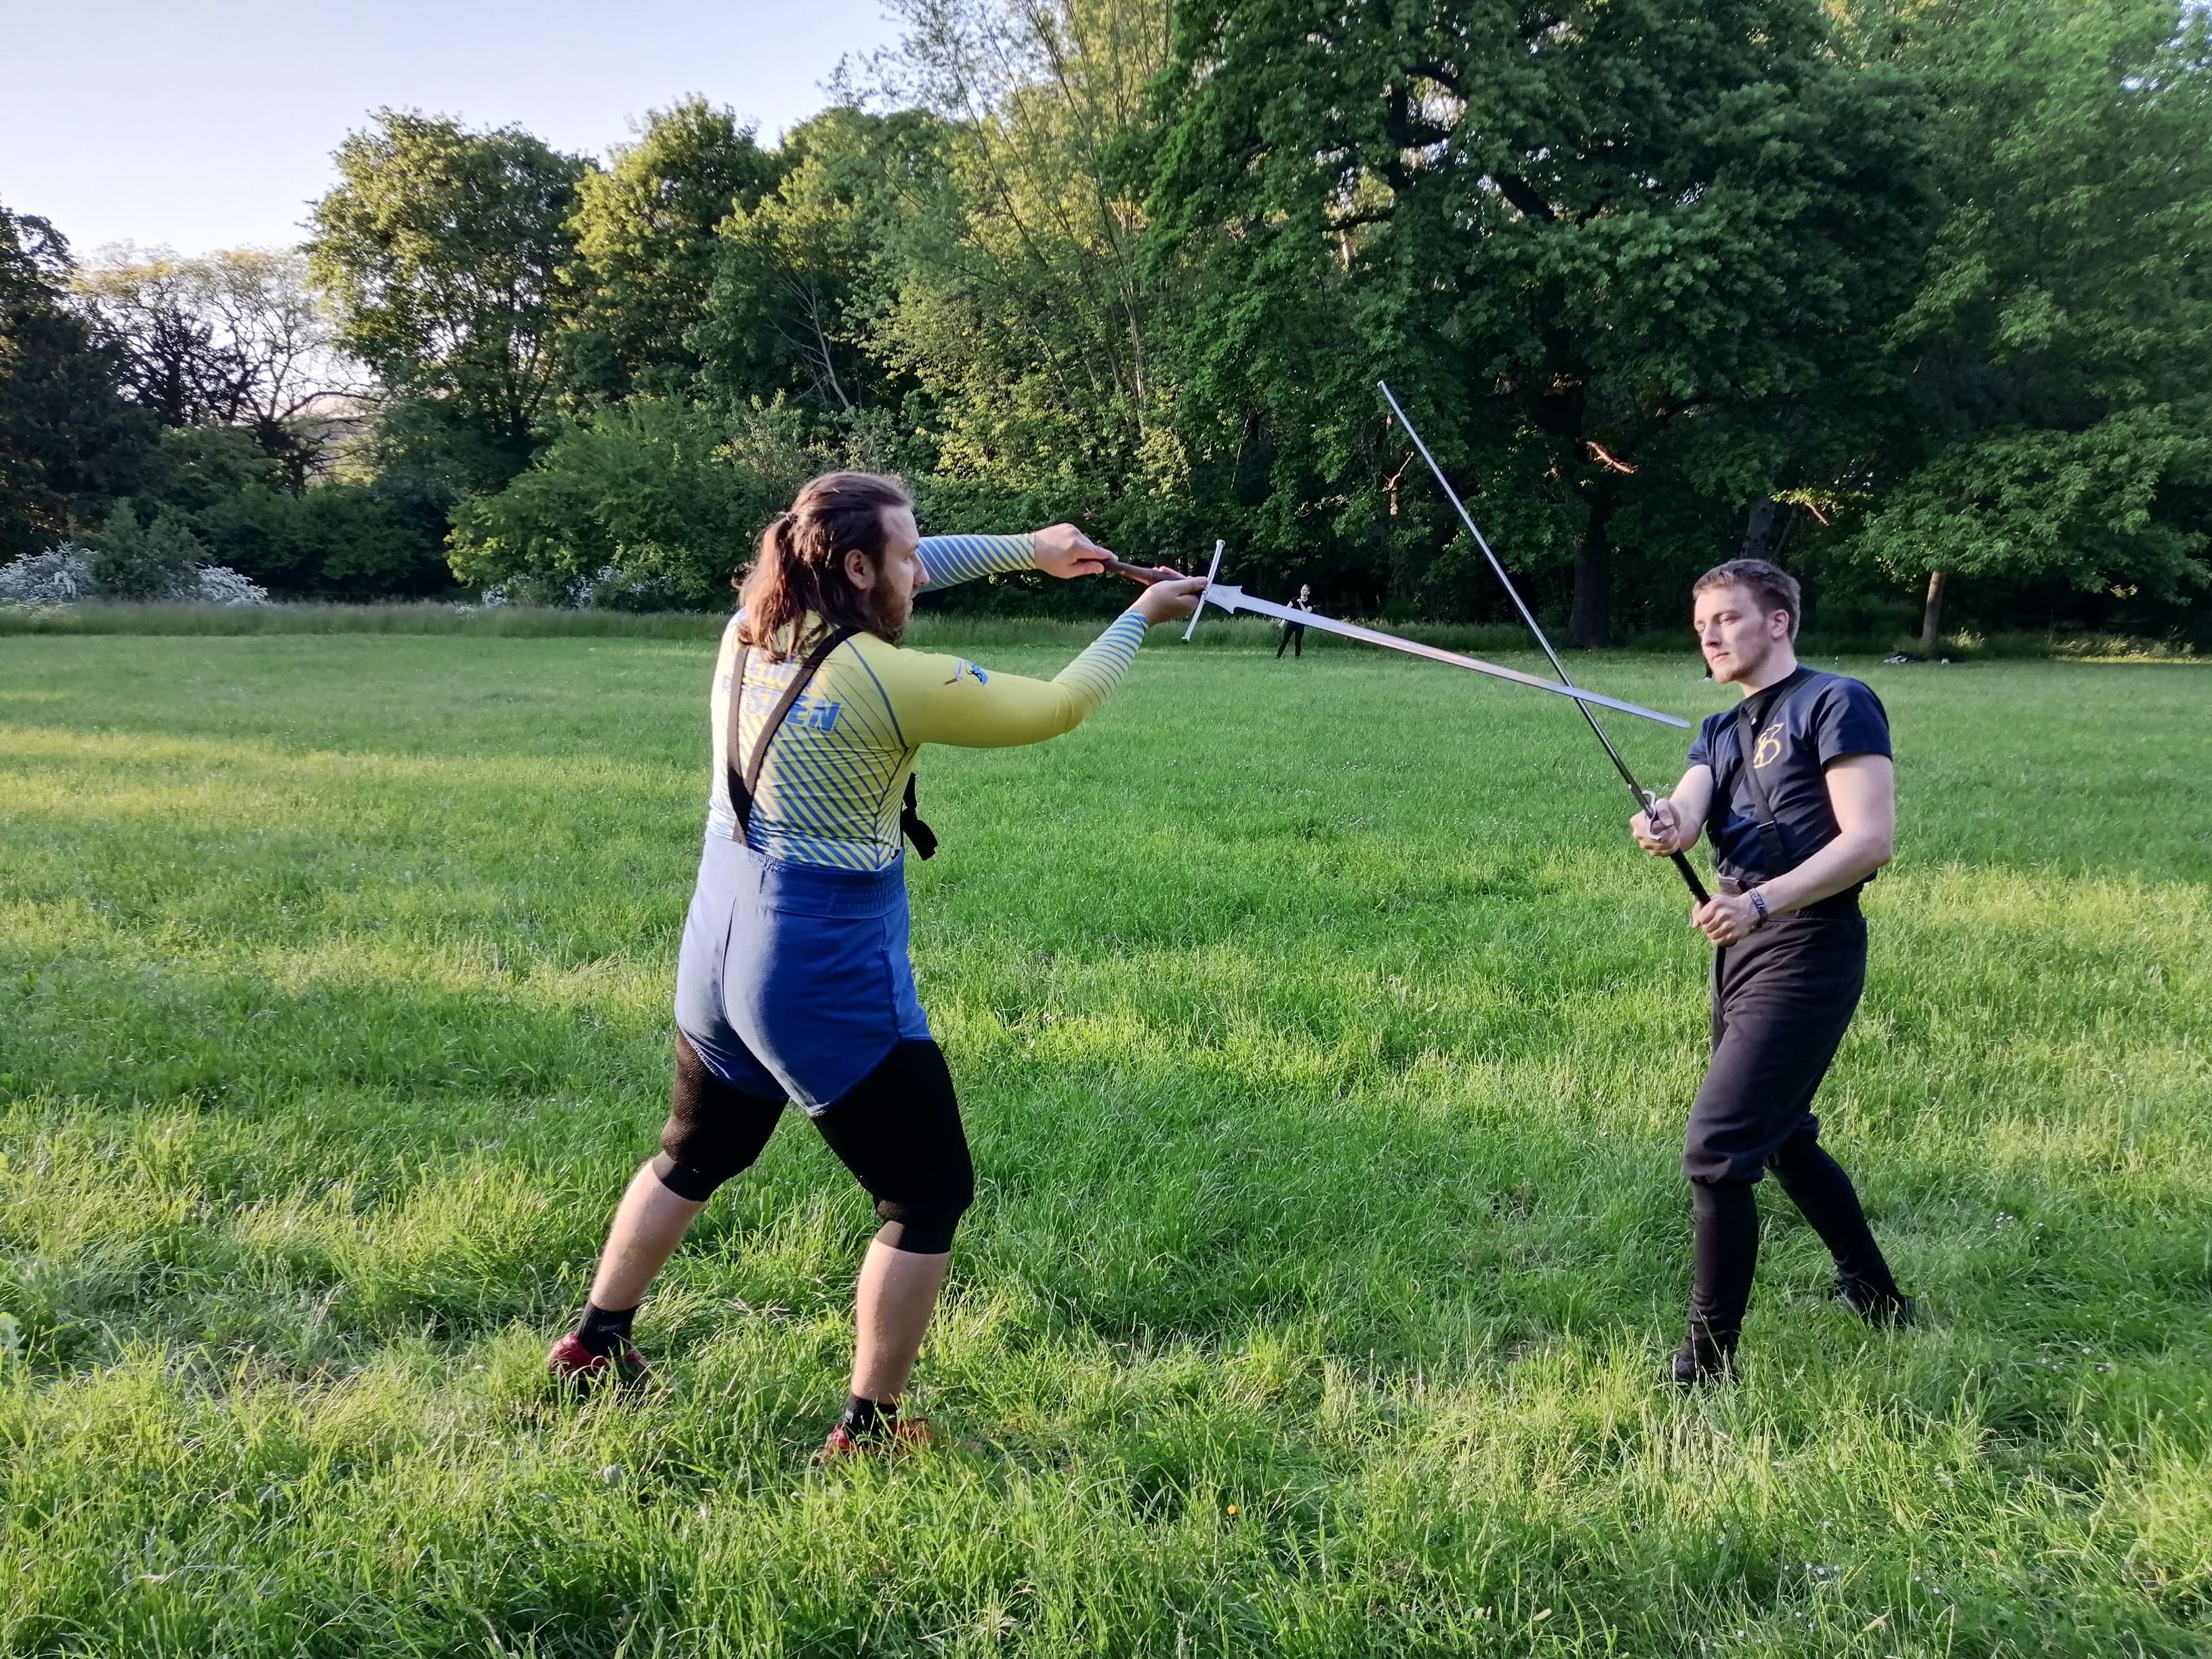
\includegraphics[width=\linewidth]{Unterhau4.jpg}
\endminipage
\end{figure}

\FloatBarrier

\paragraph{Stiche}

Stiche haben im Vergleich zu Häuen eine leicht erhöhte Reichweite und können nicht passiv gedeckt werden. Ein effektiver Stich erfordert im Vergleich zu einem Hau noch weniger Kraft. Der Nachteil an Stichen ist, dass es mit ihnen schwerer ist, Selbstschutz herzustellen.

\paragraph{Schnitte}

Schnitte besitzen bei weitem die geringste Rechweite, da die Klinge bereits auf ihrem Ziel aufliegen muss, damit ein Schnitt initiiert werden kann. Schnitte sind deshalb praktisch für enge Mensuren. Sie können Selbstschutz herstellen, indem entweder die Klinge des:der Gegner:in durch den eigenen Körper blockiert wird oder man den Schnitt gegen die Arme des:der Gegner:in ausführt und so dessen Klinge verdrückt.
\\
\\
Unterschnitt:

\FloatBarrier

\begin{figure}[!htb]
\minipage{0.24\textwidth}
    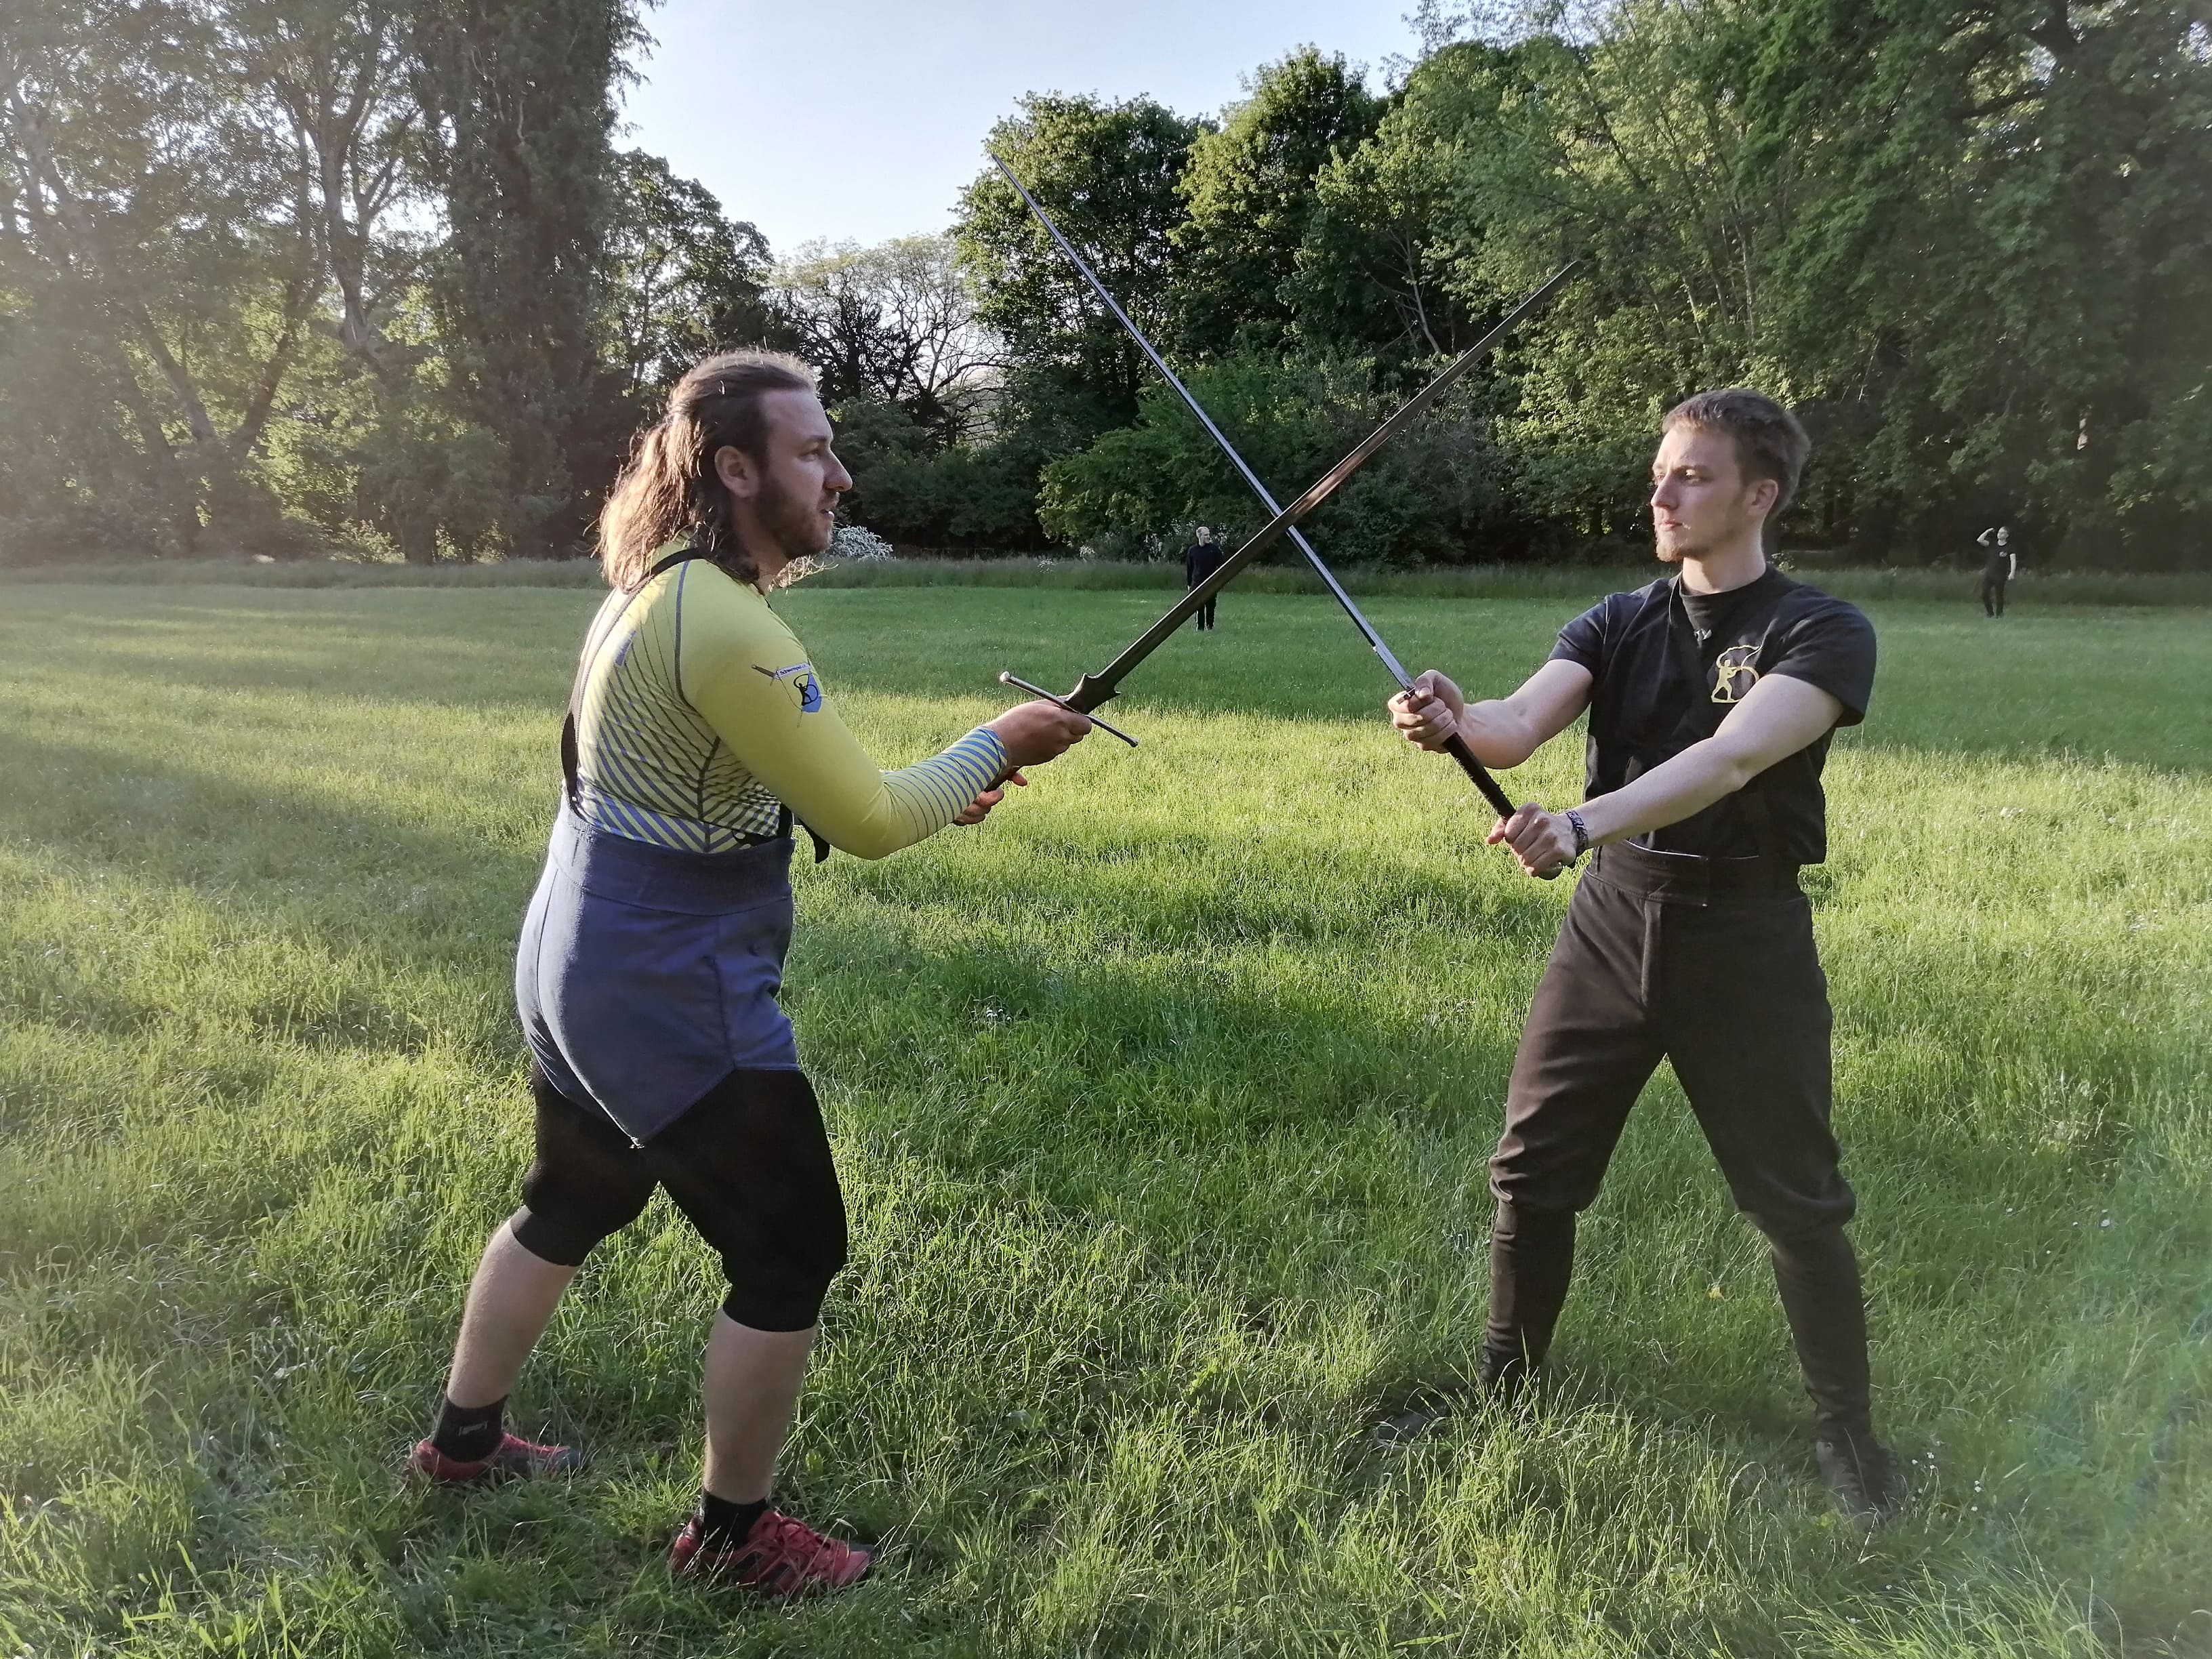
\includegraphics[width=\linewidth]{Schnitt1.jpg}
\endminipage\hfill
\minipage{0.24\textwidth}
    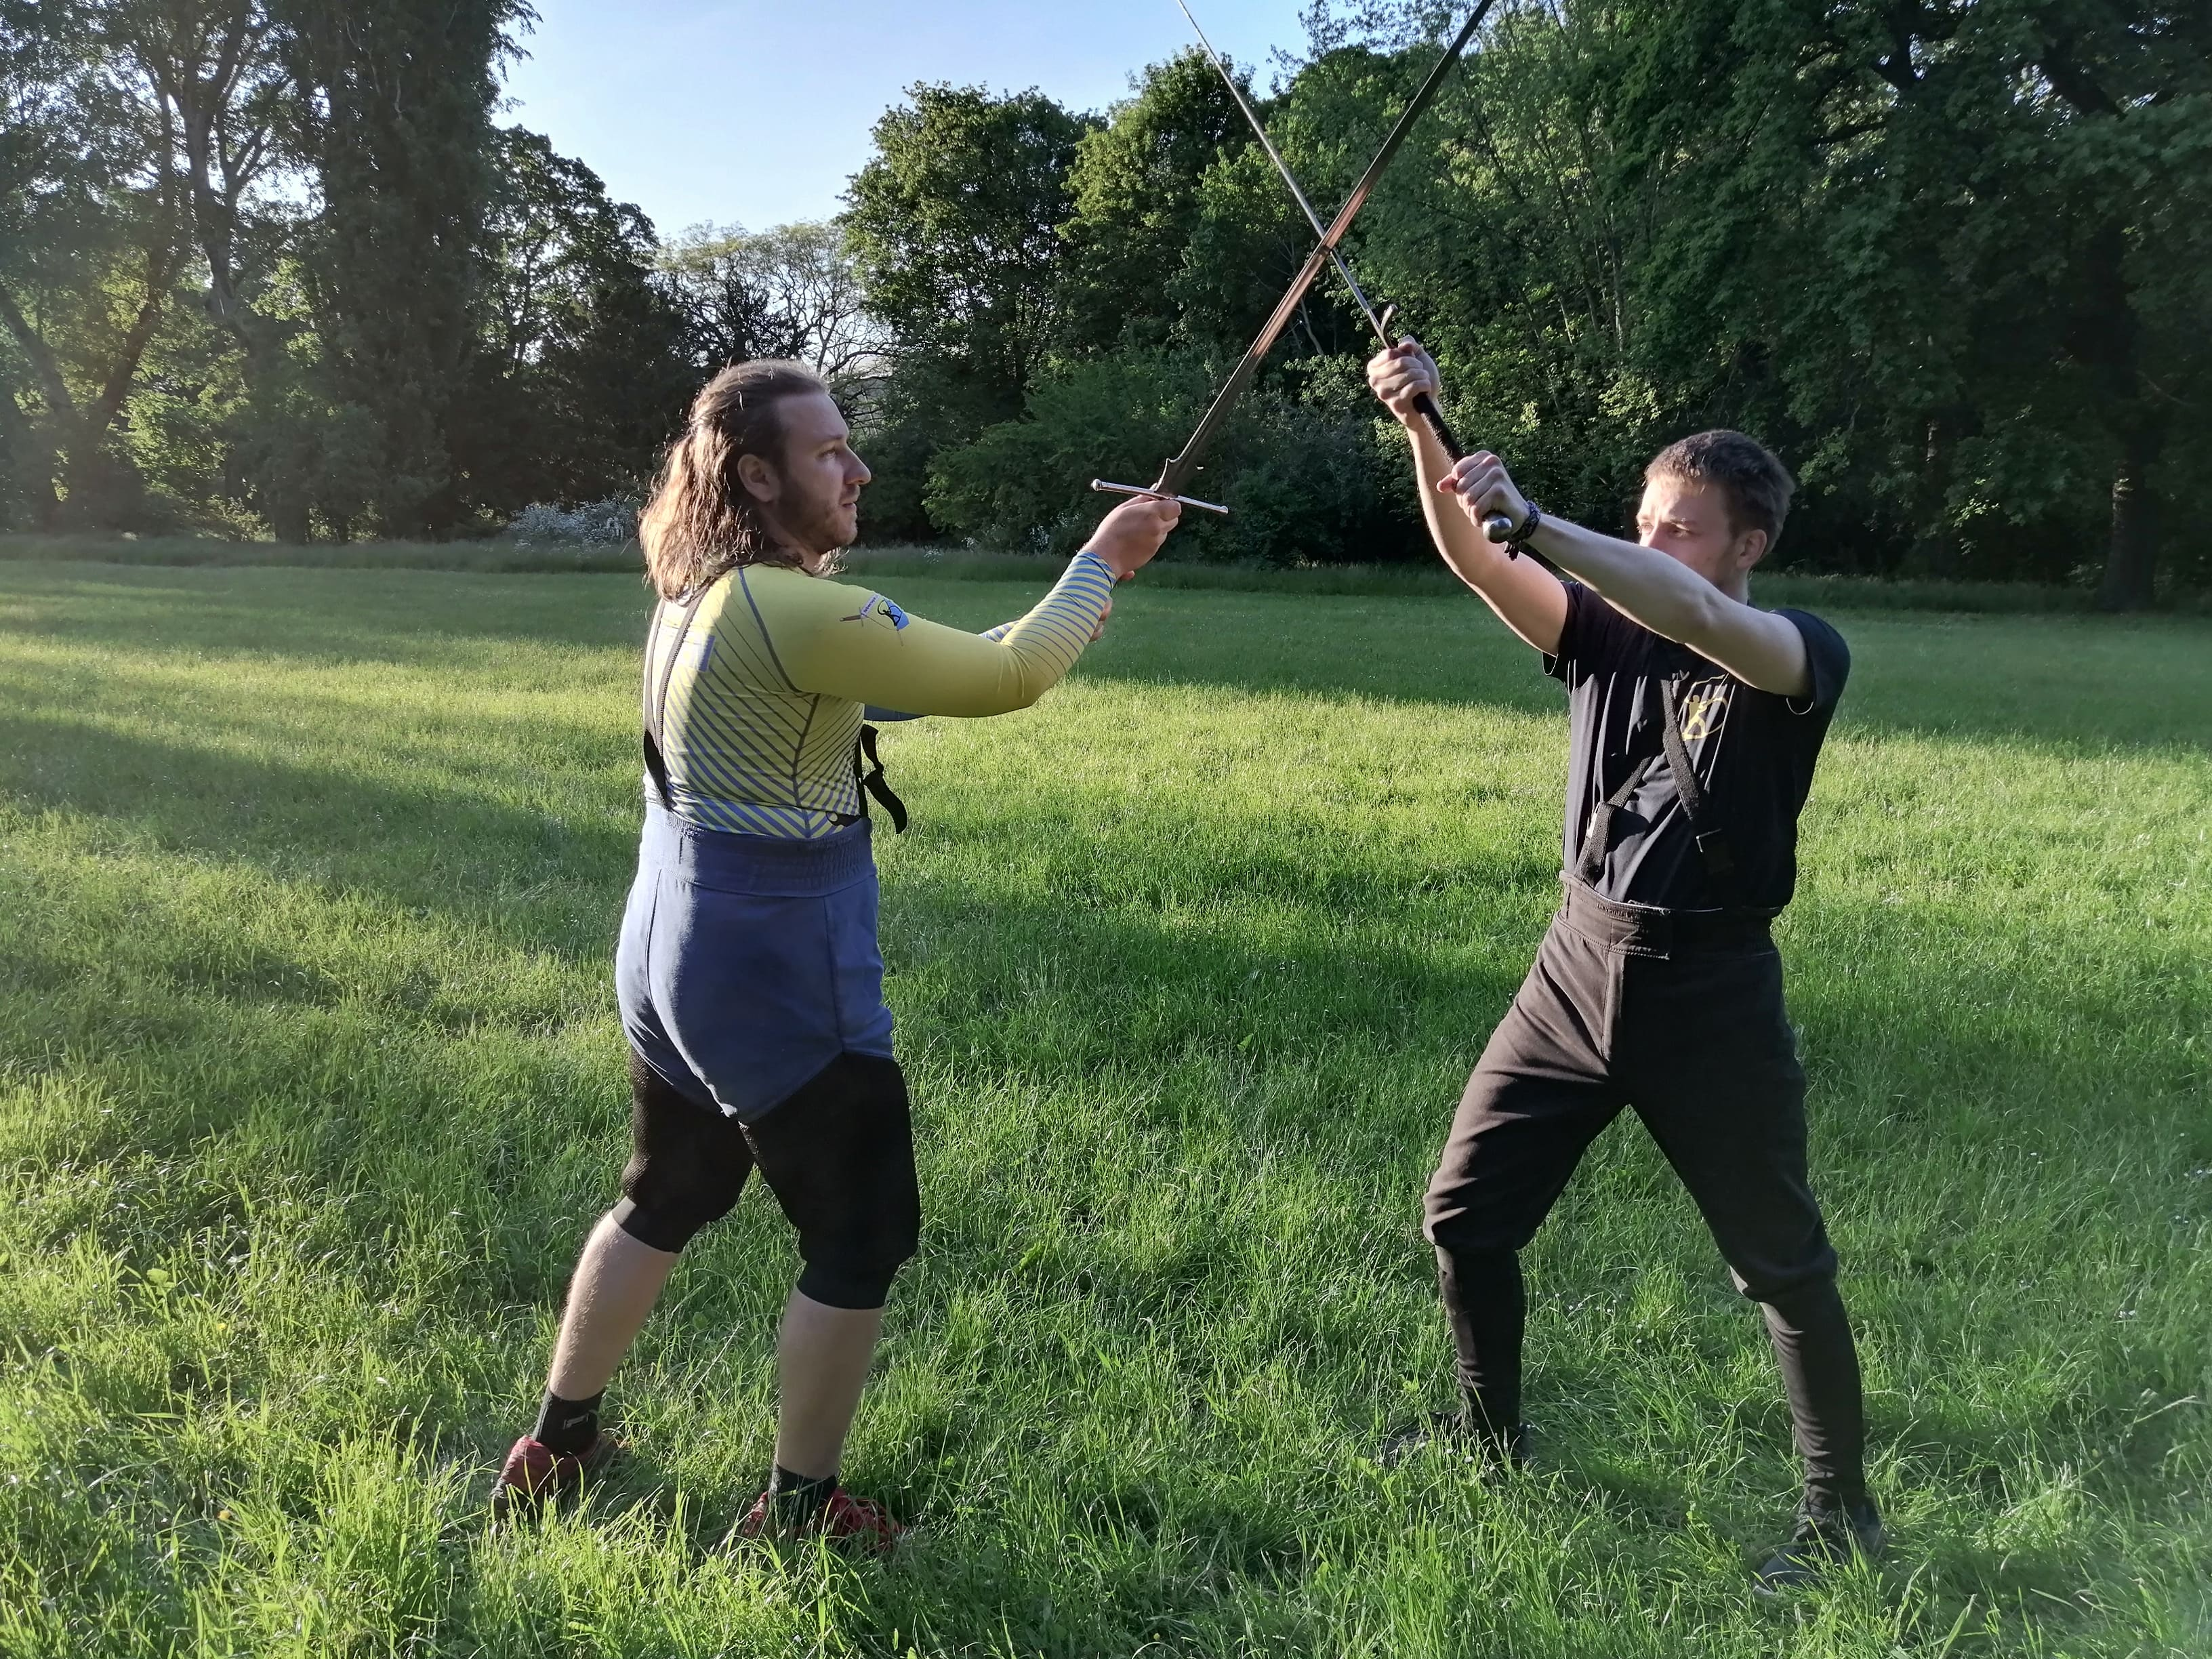
\includegraphics[width=\linewidth]{Schnitt2.jpg}
\endminipage\hfill
\minipage{0.24\textwidth}
    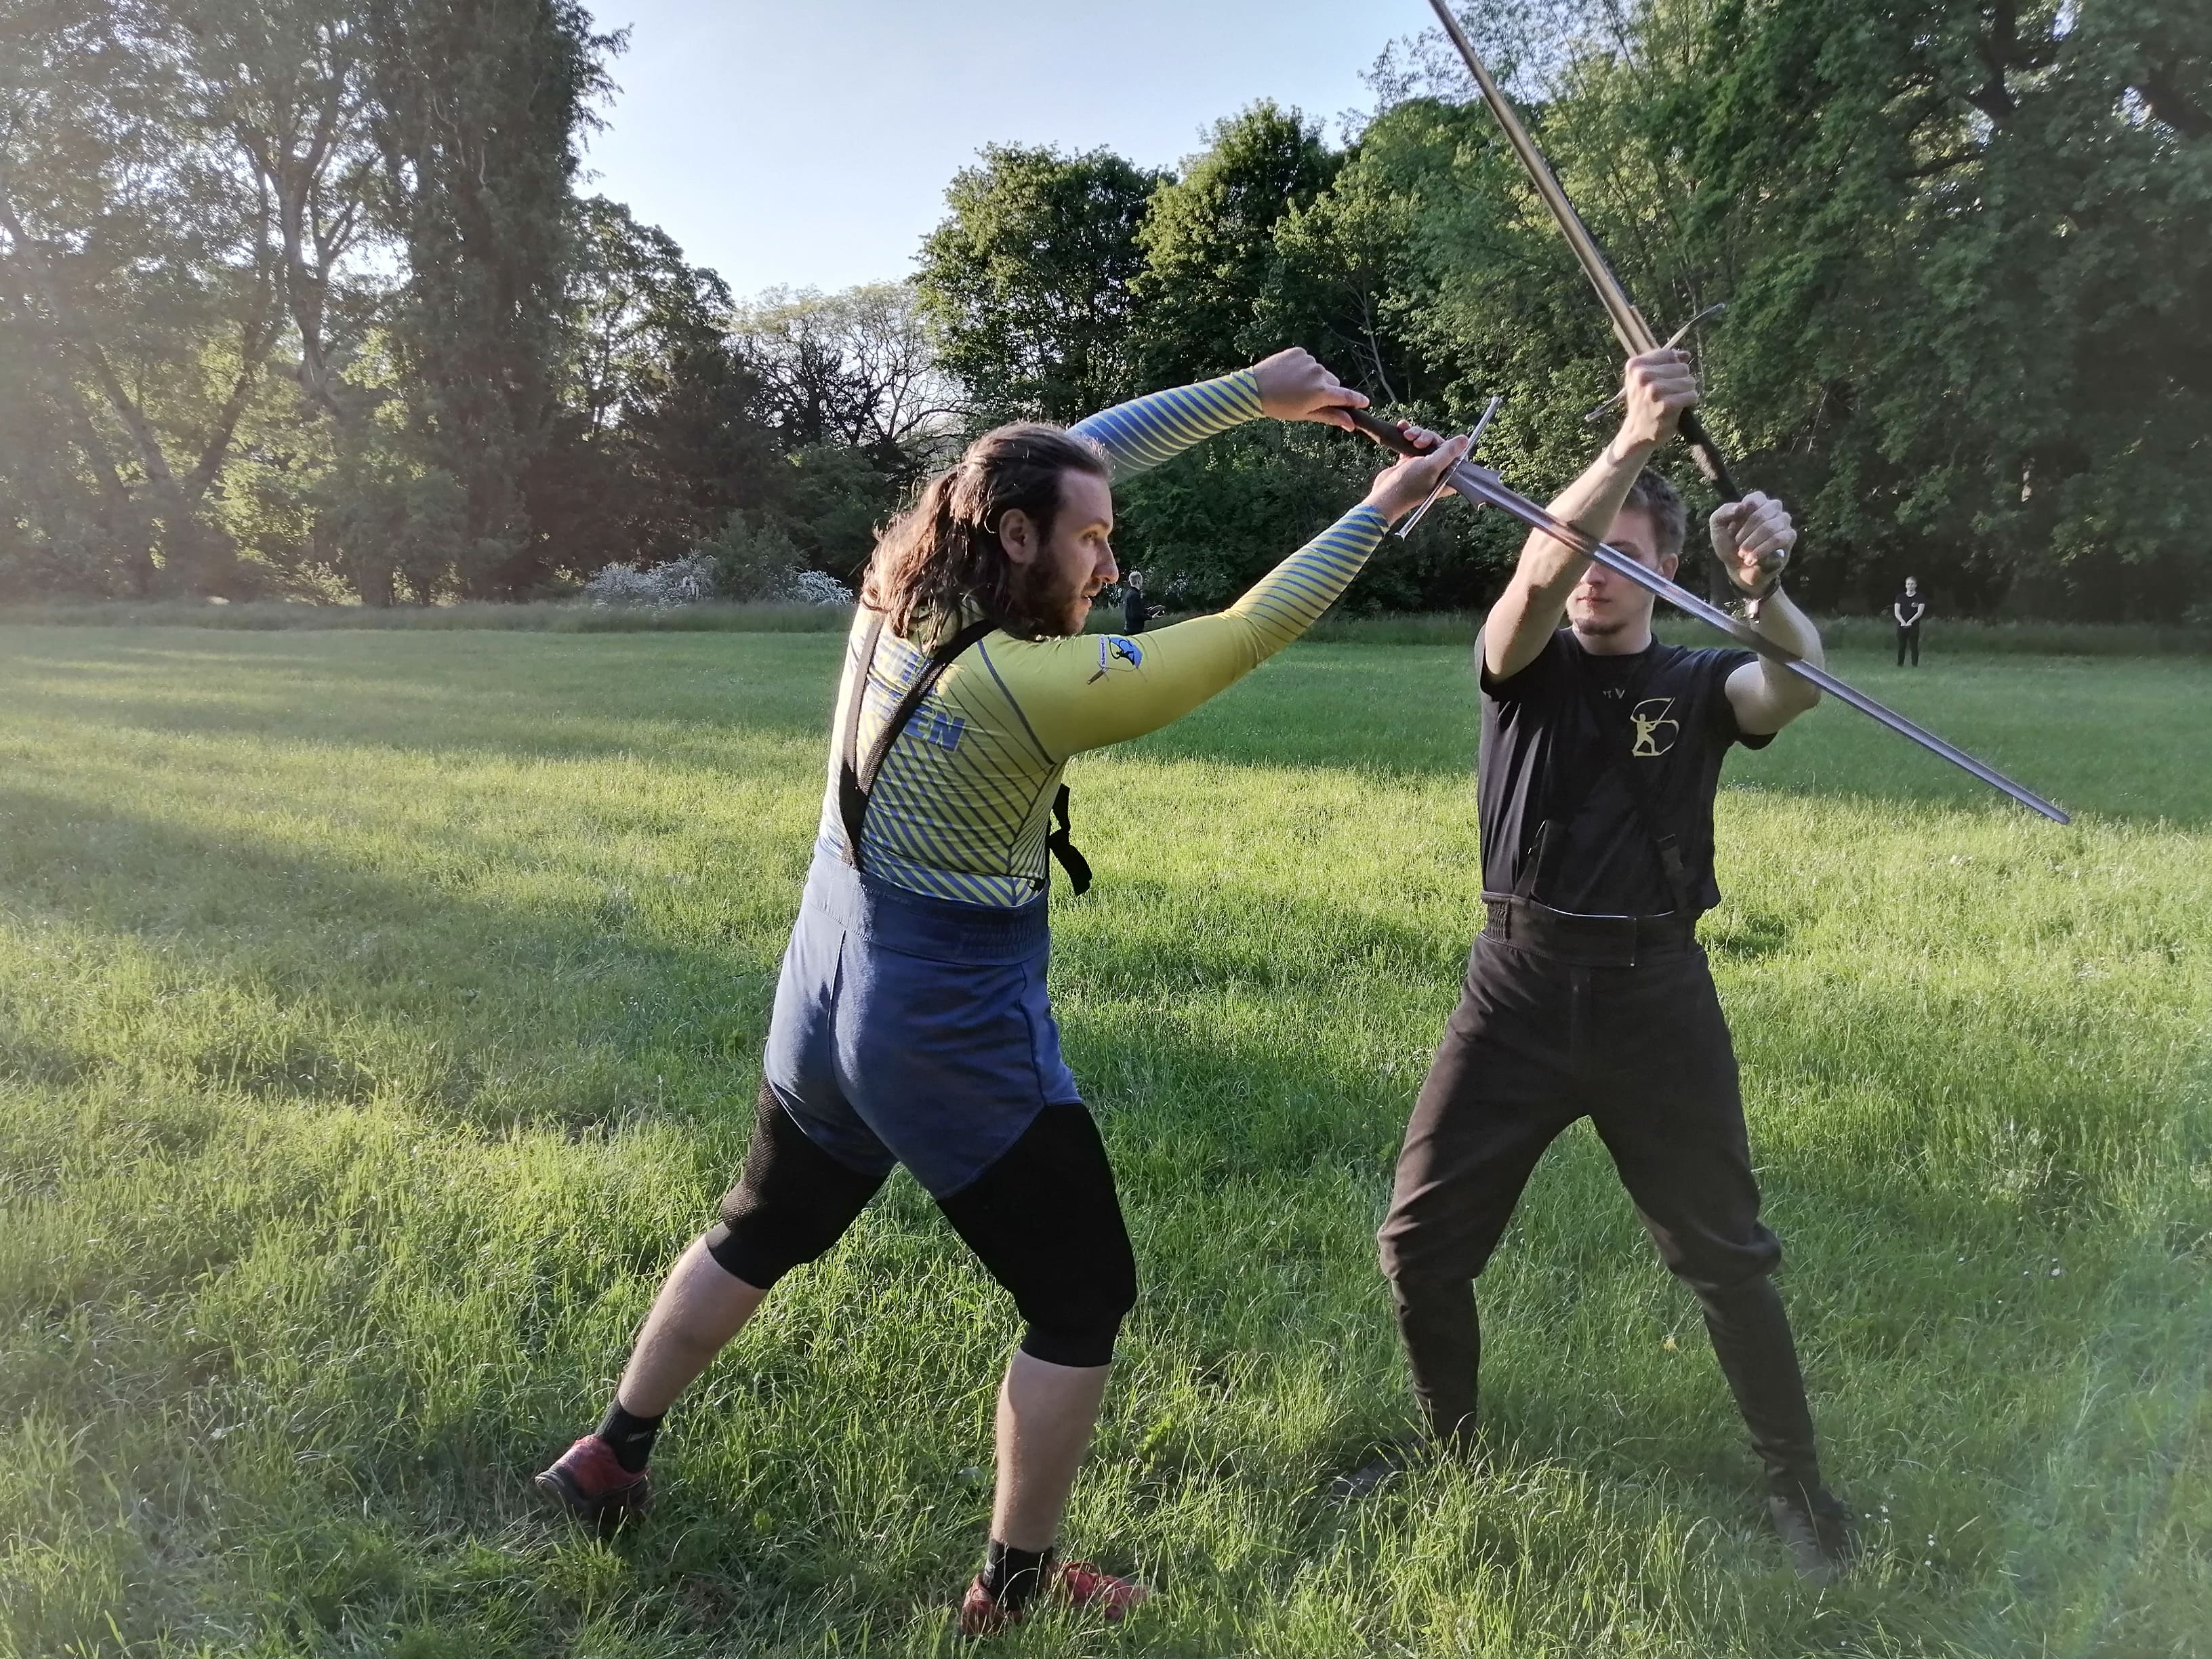
\includegraphics[width=\linewidth]{Schnitt3.jpg}
\endminipage\hfill
\minipage{0.24\textwidth}
    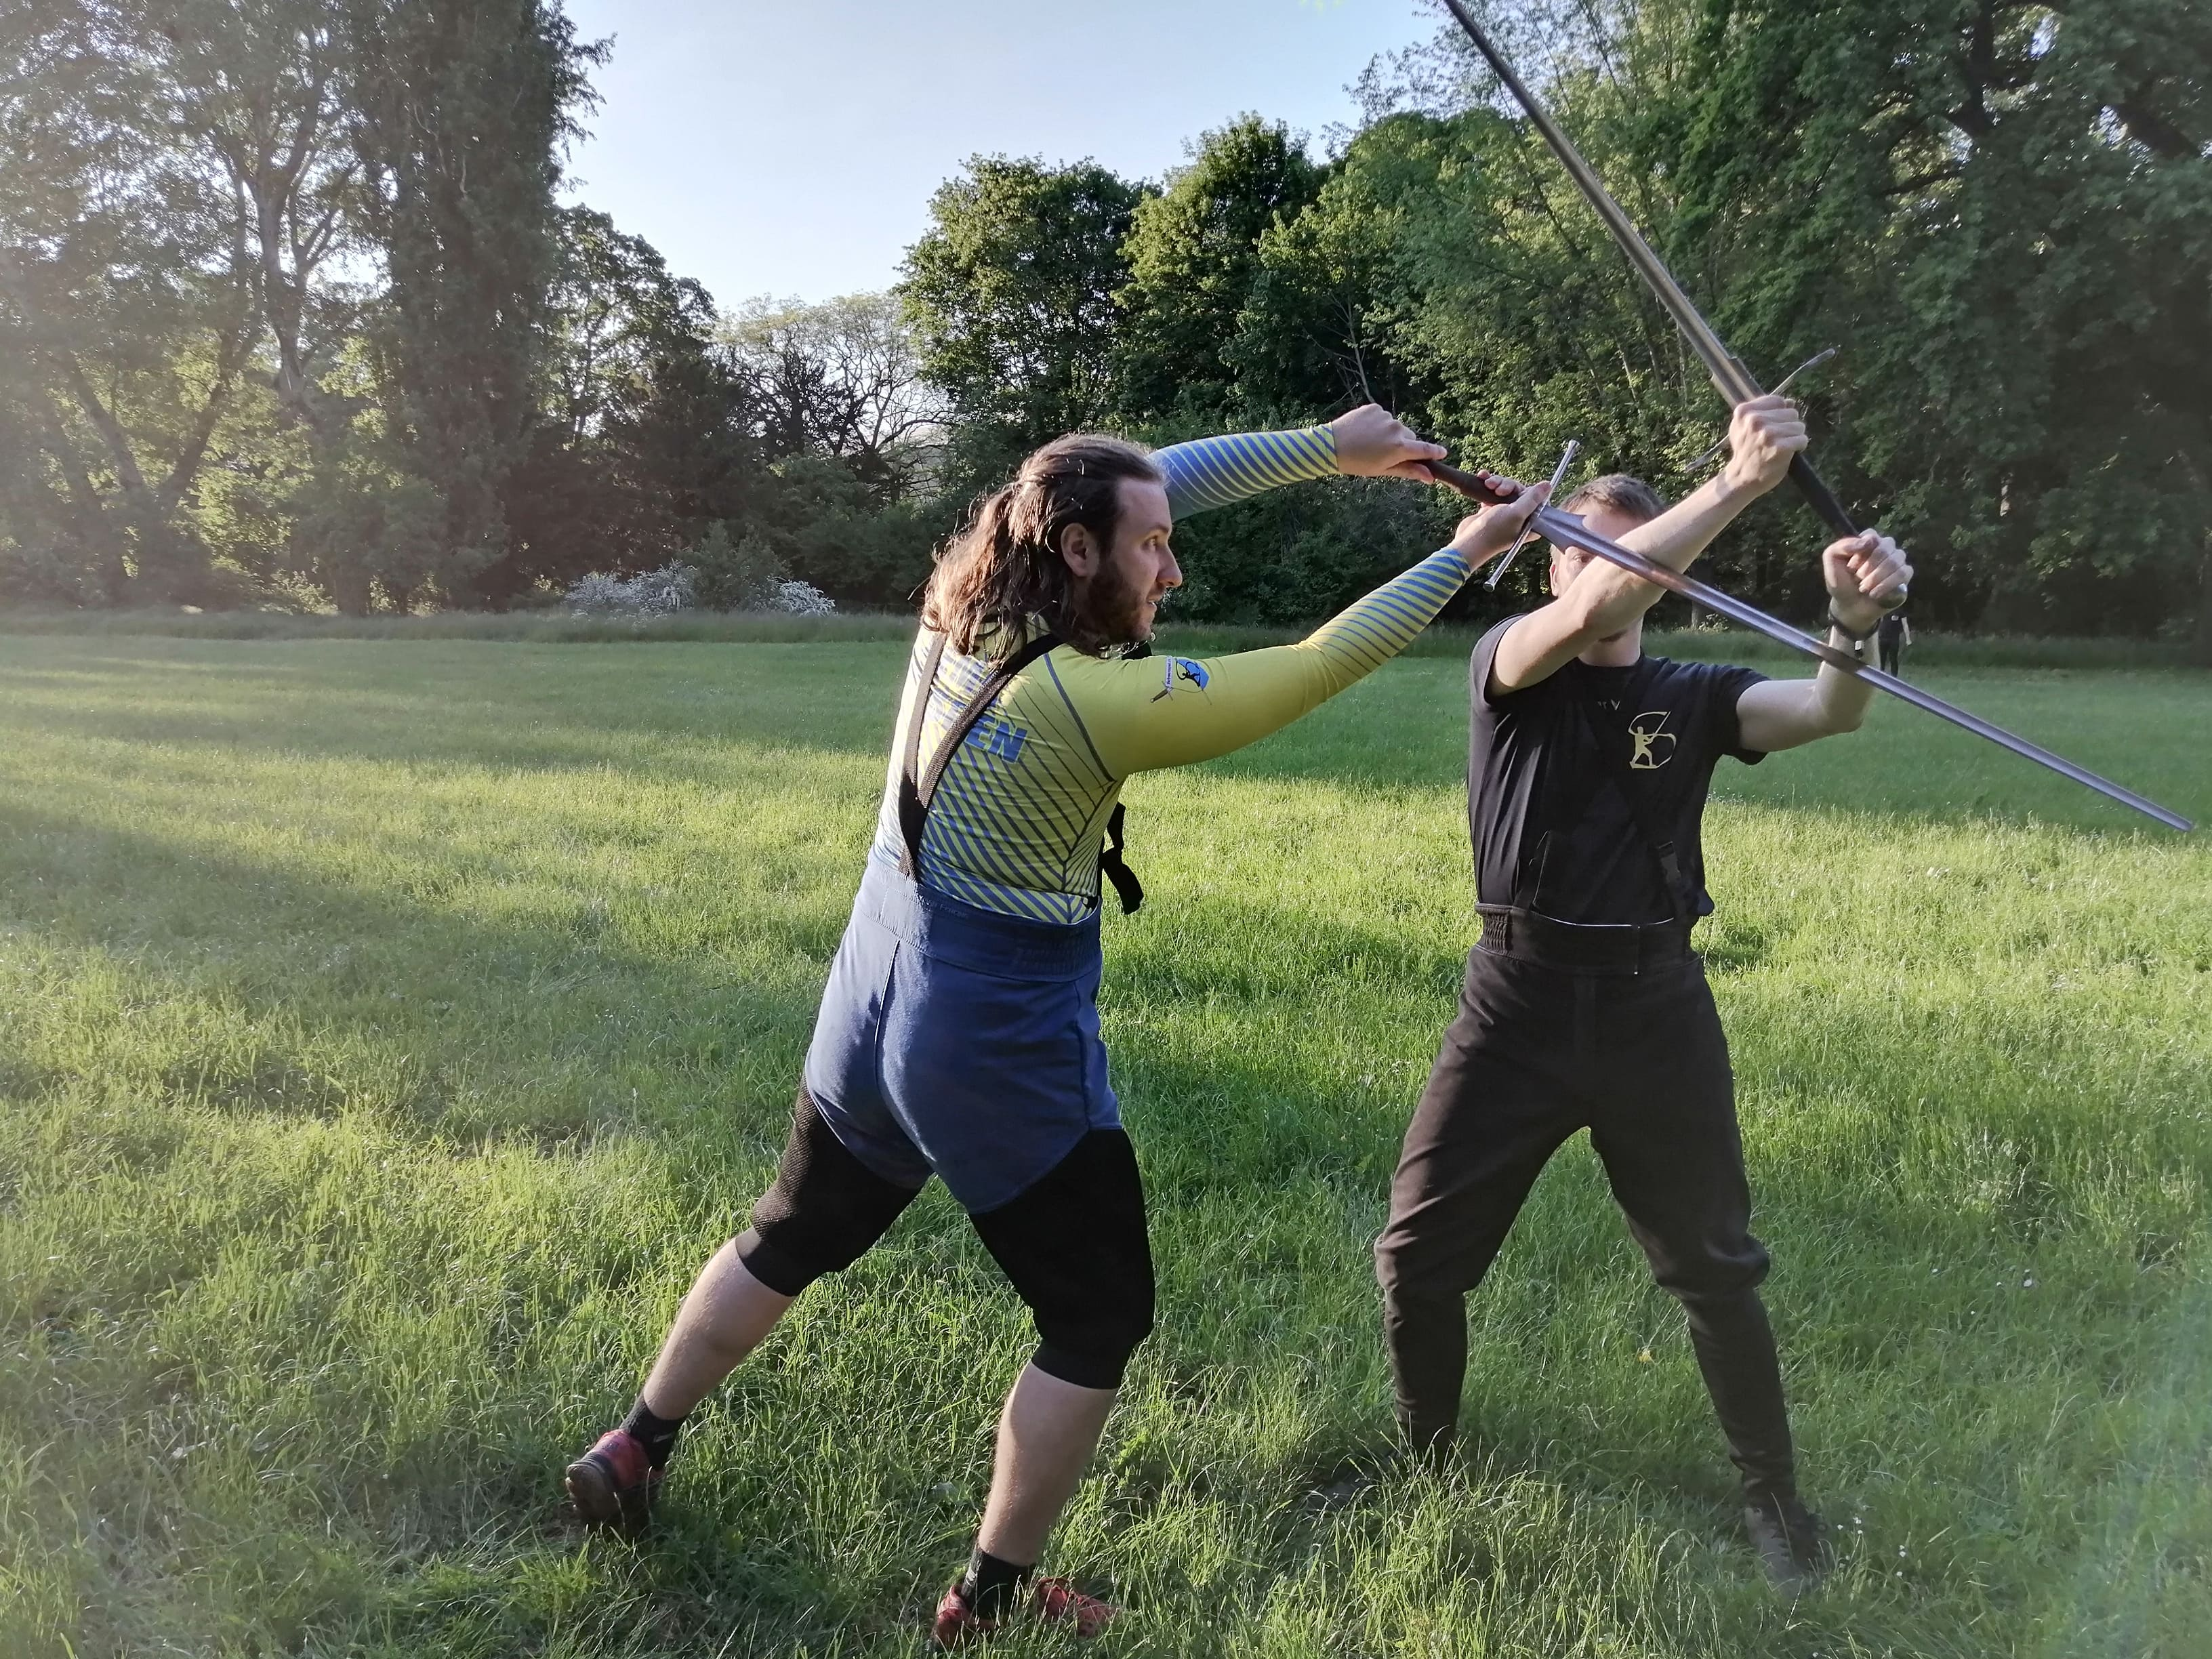
\includegraphics[width=\linewidth]{Schnitt4.jpg}
\endminipage
\end{figure}

\FloatBarrier

\newpage

\subsection{Erschließen eines Fechtstücks}

Gemäß Maxime II ist ein jeder angehalten eine persönliche Interpretationen der Lehren Liechtenauers zu finden. Um diesen Findungsprozess ein wenig Struktur zu verleihen und einige Denkanstöße zu geben sei nachfolgend ein Vorschlag zur grundlegenden Strukturierung einer Interpretation vorgestellt, so wie sie auch im Training von Schwertspiel genutzt wird. Des Weiteren befindet sich im Anhang das Interpretationskonzept nach Thore Wilkens, an welches sich auch dieses Konzept anlehnt.

\subsubsection*{I.Ursache}

Beschreibt die Ausgangsituation: Welche Hut nehmen die Fechtenden ein und warum? Das Warum sollte in der Gruppe erläutert werden.

\subsubsection*{II.Auslöser}
Beschreibt den entscheidenden Moment, der die Ausführung des Stückes initiiert. Dieser sollte in der Gruppe besprochen werden, da dieser Auslöser später in Übungen genau erschlossen werden soll.

\subsubsection*{III.Ausführung}

Beschreibt die eigentliche Ausführung des Stücks: Diese soll in der Gruppe anhand der fechterischen Grundprinzipien ausführlich besprochen werden. Dies geschieht anhand von „Show and Tell“ durch die Fechter:innen im Dialog mit dem:der Trainer:in. Diese:r wirft das Augenmerk auf Mensur, Beinarbeit, Schwerthaltung und auf Beachtung der fechterischen Grundprinzipien.
\\
\\
Schließlich wird die gefundene Interpretation noch einmal von den Trainer:innen vorgeführt. Anschließend haben die Fechter:innen in den folgenden Trainingseinheiten die Möglichkeit ihre persönliche Interpretation zu finden und zu festigen. Der Fokus der Übungen sollte Anfangs mehr auf dem Konditionieren des Auslösers liegen. Statische Übungen können dann genutzt werden bis alle Fechter:innen eine saubere Ausführung beherrschen. Anschließend wird der Auslöser in dynamischen Übungen wieder in den Fokus gesetzt. Schließlich kann das Fechtstück in offeneren dynamischen Übungen zusammen mit anderen Stücken in einen größeren Kontext gesetzt werden.

\newpage
